\documentclass{hebrew-academic-template}
\addbibresource{refs.bib}

% Define version command for use in footers
\newcommand{\version}{\en{Version 9.0}}

\begin{document}

% Custom title page with version and image
\begin{titlepage}
  \null\vfil
  \begin{center}
    \texthebrew{\LARGE\bfseries בינה מבוזרת: סוכנים אוטונומיים בעידן הבינה המלאכותית}\par
    \vskip 1em
    \textenglish{\Large\bfseries Distributed Intelligence: Autonomous Agents in the Age of AI}\par
    \vskip 3em
    {\large ד"ר יורם סגל \par}
    \vskip 0.5em
    {\large \textenglish{©} \textenglish{Dr. Yoram Segal} - כל הזכויות שמורות \par}
    \vskip 2em
    {\large \hebyear{2025} \par}
    \vskip 1em
    {\large \en{Version 9.0} \par}
    \vskip 2em
    \en{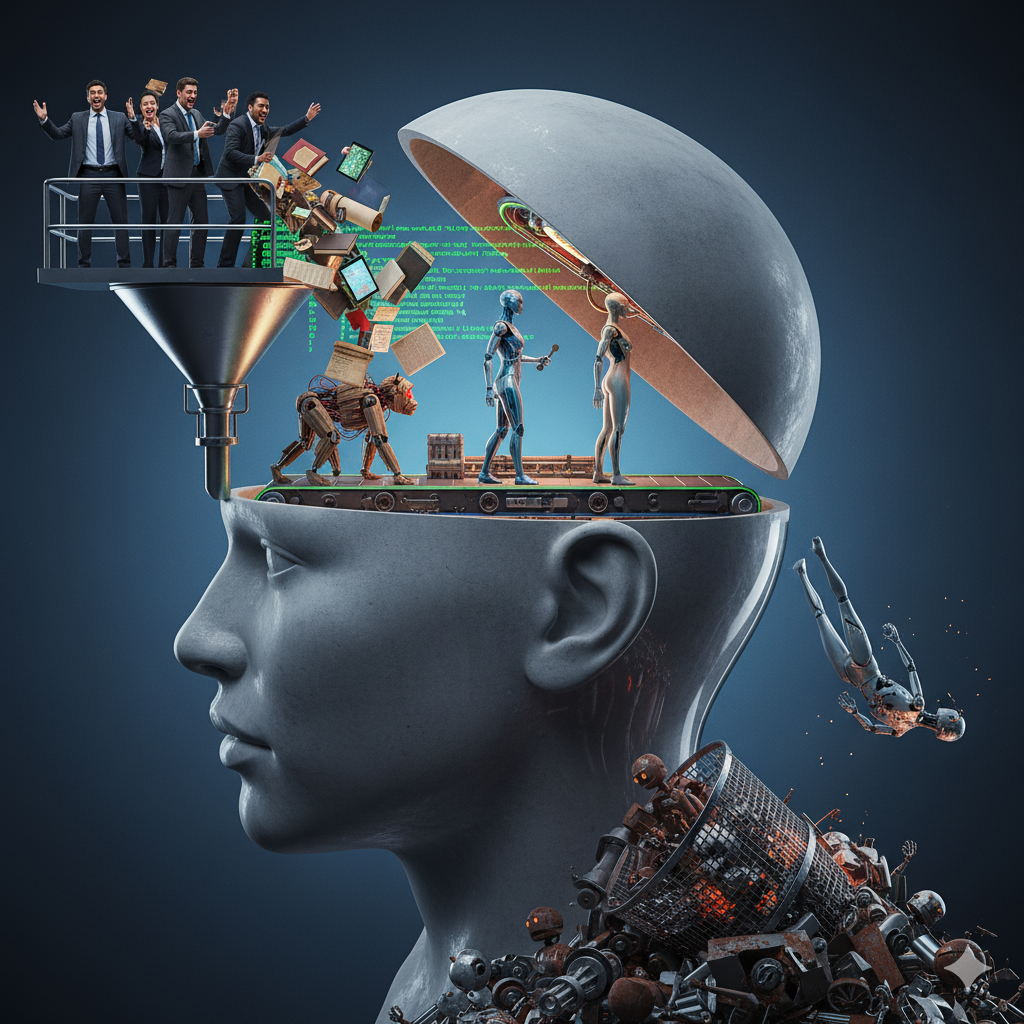
\includegraphics[width=0.75\textwidth]{images/פס יצור של סוכני AI.png}}
  \end{center}
  \vfil\null
\end{titlepage}

% Back Cover Page
\newpage
\thispagestyle{empty}
\begin{center}
{\Large \textbf{גב הספר}}
\end{center}
\vspace{1em}

האדם המציא את הכתב כדי לא לשכוח את חוקותיו; זו הייתה המהפכה הקוגניטיבית שאיפשרה ציוויליזציה. היום, אנו ניצבים מול פרדוקס עמוק: סוכני ה\en{-AI} המתוחכמים ביותר סובלים מטרגדיה קיומית המכונה "האלצהיימר של המכונה", והופכים את כל עמלנו הדיגיטלי לזמני וחסר ערך.

זהו ספר על פירוק המונולית והכרזה על ארכיטקטורה מבוזרת חדשה, הנסמכת על הטכנולוגיה החדישה ביותר נכון לאוקטובר \num{2025}. הדיון קופץ מהרהור פילוסופי המציג את השפעת סוכני ה\en{-AI} באנלוגיה לספר קוהלת, אל מול פרקטיקות מימוש באמצעות קוד פייתון: כיצד נבטיח את יציבות סוכני ה\en{-AI} כאשר נוסחאות מתמטיות וטרנספורמציות לינאריות מזהירות מפני כשל? הוא מפרק את השאלה על הבל האופטימיזציה וממיר אותה לתוכנית בנייה מעשית: הדרך היחידה ליציבות עוברת דרך מודולריות וארכיון.

דרך קוד פייתון והטמעת \en{SDK} מתקדמים, אנו לומדים להנדס את ארבעת הקבצים – זיכרון חיצוני המאפשר לכל סוכן לזכור את הנרטיב המלא של הפרויקט. האורכסטרציה של סוכנים הופכת למקהלת הסוכנים באמצעות פרוטוקול \en{MCP}, אך זו רק ההתחלה. הספר מתריע מפני ניוון מיומנות, החרב הפיפיות של האוטומציה היתרה, ומקדיש דיון נוקב לאתיקה ואבטחה הנדרשת להשגת \en{Alignment} מול הסכנה שסוכני ה\en{-AI} ישכחו את פרטיותנו. תפקידנו אינו להתחרות באלגוריתם, אלא להבטיח שבבניית עולם חדש זה, נשמור על הממדים הלא-אלגוריתמיים: רצון חופשי, חמלה, ונרטיב. האם נבנה סוכנים שישרתו אותנו לרגע, או שותפים שיזכרו את מהותנו?

\textbf{למי מיועד הספר:}

\begin{itemize}
\item \textbf{למהנדס ולמתכנת:} הספר מציג קוד פייתון מפורט ופתרונות \en{SDK} עדכניים, וכן נוסחאות מתמטיות לניתוח יציבות המערכת, המהווים בסיס מוצק לבניית סוכני \en{AI} אחראיים.
\item \textbf{לאנשי הגות ופילוסופיה:} הספר מציע מסגרת פילוסופית קיומית הבוחנת את המתח בין החרדה האנושית להתפעמות הטכנולוגית, ודן בנושאי יראת האלגוריתם ומשמעות הנרטיב בעידן האוטומציה.
\item \textbf{לקורא הכללי:} מסע מרתק המשלב היסטוריה, אתיקה וטכנולוגיה, שיעניק לכם את הכלים להבין, ולעצב, את גורל הציוויליזציה הדיגיטלית המתהווה.
\end{itemize}

\textbf{על המחבר,}

\textbf{ד"ר יורם סגל:} בנקודת המפגש הנדירה שבין הקוד לבין המתמטיקה של הגוף.

הוא התחיל את מסע ה\en{-AI} עם מחקר בתחום תנועת אדם בוידאו דיגיטלי. עבודת הדוקטורט שלו הייתה תרגום פורץ דרך של תנועת האדם – מכאב או ריצה – לגיאומטריה קרה ולנוסחאות שאינן משקרות. תובנה זו – שהקיום כפוף למבנה – היא המכוננת את גישתו ל\en{-AI}.

במשך למעלה מעשרים שנה, ד"ר סגל גילה את הסודות הללו גם בשדה הקרב הטכנולוגי: הוא זה שפועל בתווך שבין הוראה באוניברסיטאות בן גוריון, רייכמן ובר-אילן, לפרסום מחקרים בכתבי עת רפואיים, ולפרקטיקה יומיומית בתעשייה. הוא שימש כמייסד ומנהל מיזם הזנק של בינה מלאכותית, שם הוביל הטמעת \en{AI} באירגונים ובניית מערכות מרובות סוכנים מורכבות. הוא מכיר את גבולות הקוד, נושא בפטנטים אמריקאיים ומוגדר כיועץ מומחה להוריזון אירופה.

זוהי הסיבה מדוע הספר הזה הוא מסמך הנדסי פילוסופי המייצג את המילה האחרונה בטכנולוגיה: הוא נכתב על ידי מי שמבין את הדילמה מכל צדדיה. הוא המורה והבנאי שמוכרח להזהיר אותנו. הוא יודע בדיוק איך לכתוב את קוד הפייתון שמוביל לניוון מיומנות, ולכן הוא היחיד שיכול להציע את הדרך להנדס מערכות אתיות. ד"ר סגל מציע לנו דרך לפעול, אך דורש מאיתנו לזכור: השאלה הגדולה באמת היא לא האם סוכני ה\en{-AI} יכולים לבצע את המשימה, אלא האם אנחנו זוכרים מה תפקידנו אל מול הבל המודל.

הספר הזה הוא התוצאה של אותה כנות אינטלקטואלית בלתי מתפשרת: חזון שנכתב על ידי מי שמבין איך לבנות את המערכת, ולכן יודע בדיוק איך לשמור בה את האנושיות. הוא מגיע לכאן כדי להעניק לנו את הידע החסר ביותר: לא רק איך ליצור סוכני \en{AI} יעילים, אלא איך לשלוט בהם באחריות.

% Override footer to replace default name
\fancyfoot[LE]{\en{\thepage}}
\fancyfoot[RO]{\en{\thepage}}
\fancyfoot[RE]{\en{©} \en{Dr. Yoram Segal} - כל הזכויות שמורות - \version}
\fancyfoot[LO]{\en{©} \en{Dr. Yoram Segal} - כל הזכויות שמורות - \version}

\newpage
\begin{abstract}
בעשור האחרון אנו עדים למעבר מפרדיגמת בינה מלאכותית יחידה למערכות המורכבות מצוות של סוכנים מתמחים. ספר זה בוחן לעומק שינוי פרדיגמה זה במבנה של \textbf{ארבעה חלקים משלימים}:

\textbf{חלק א'} (פרקים \num{1}–\num{6}) עוסק בארכיטקטורת הקוגניציה המבוזרת (תת-סוכנים) וכיצד פלטפורמות דוגמת \en{Claude CLI} ופרוטוקול \en{MCP} מאפשרים שיתוף פעולה חלק בין סוכנים מרובים.

\textbf{חלק ב'} (פרקים \num{7}–\num{13}) עובר לממד הקוגניטיבי: כיצד סוכנים שומרים על זיכרון, עקביות ורציפות לאורך זמן באמצעות מערכות זיכרון חיצוניות מובנות (ארבעת הקבצים: \en{\texttt{PRD.md}}, \en{\texttt{CLAUDE.md}}, \en{\texttt{PLANNING.md}}, \en{\texttt{TASKS.md}}).

\textbf{חלק ג'} (פרקים \num{14}–\num{16}) משלים את התמונה: כיצד ניתן לארוז מומחיות פרוצדורלית ליחידות מודולריות (\en{Skills}) הניתנות לשימוש חוזר? נדון בעקרון \en{Progressive Disclosure} (חשיפה הדרגתית), נבחן את היתרונות של ארכיטקטורה מבוססת תיקיות קבצים, ונעמוד על הסכנות הטמונות באוטומציה יתר – תופעת ניוון המיומנות (\en{Skill Atrophy}).

\textbf{חלק ד'} (פרקים \num{17}–\num{20}) סוגר את הספר במסגרת פילוסופית קיומית המבוססת על ספר קהלת. באמצעות השיטה הפרשנית העתיקה של פשט, דרש וסוד, אנו בוחנים את המתח הקיומי בין החרדה האנושית להתפעמות הטכנולוגית. נדון בהבל האופטימיזציה האינסופית, זמניות המודלים (\en{Planned Obsolescence}), משבר ה\en{-Alignment}, ויראת האלגוריתם. החלק מסתיים במסר מרכזי: תפקידנו אינו להתחרות באלגוריתם, אלא לשמור על הממדים הלא-אלגוריתמיים של הקיום – נרטיב, חמלה, ורצון חופשי.

נעסוק גם בהיבטי אתיקה, פרטיות וסיכונים הכרוכים בסוכני \en{AI}, ונדגים את הדיון באמצעות מקרה מבחן מעשי – סוכן לחילוץ מידע מ\en{-Gmail}. הספר מציג \textbf{שני מסלולי יישום}: גישה ידנית מלאה (נספחים א–ד) המלמדת את יסודות הפרוטוקול, וגישה מבוססת \en{MCP Python SDK} (נספחים ה–ו, דורשת \en{Python 3.10+}) המציעה פיתוח מהיר יותר.

שילוב זה של פרספקטיבה בין-תחומית, עומק טכני, דיון היסטורי-פילוסופי וניתוח מתמטי ברמת מחקר מתקדמת, נועד להעניק לקורא הבנה רחבה ומעמיקה של הדור החדש של סוכני הבינה המלאכותית – מארכיטקטורה לזיכרון ומודולריות, ומכלי רגעי לשותפות קוגניטיבית ארוכת-טווח המבוססת על מומחיות ניתנת לאריזה.
\end{abstract}

\newpage
\tableofcontents

\newpage
\part{בינה מבוזרת - ארכיטקטורה ופרוטוקולים}
% Part 1: Distributed Intelligence - Architecture and Protocols

\hebrewsection{מבוא: שחר עידן הרב-סוכנים}

\hebrewsubsection{מהמהפכה הקוגניטיבית לשיתוף פעולה דיגיטלי}

\begin{quote}
לאורך ההיסטוריה נבדל \textit{\en{Homo sapiens}} ביכולתו הייחודית לשתף פעולה בגמישות בקבוצות גדולות. מן ה\textbf{מהפכה הקוגניטיבית}, שבה \textbf{מיתוסים משותפים} אפשרו לכידות שבטית, דרך המהפכה החקלאית והתעשייתית שאירגנו מחדש את החברה סביב צורות ייצור חדשות – ההתקדמות האנושית הוגדרה תדיר על-ידי המערכות שבנינו כדי לעבוד יחד. כעת אנו ניצבים על סף מהפכה חדשה, שבה השותפים לשיתוף הפעולה אינם בני-אנוש בלבד. אנו מעצבים עולם של תודעות דיגיטליות, והופעתן של ארכיטקטורות תת-סוכנים (\en{sub-agent architectures}) מסמנת רגע מכריע בנרטיב זה – מעבר מישות \textbf{\en{AI}} יחידה ומונוליתית לאקוסיסטמה שיתופית של סוכנים מתמחים ואינטליגנטיים\cite{Harari2018}.
\end{quote}

ספר זה מתעד את המעבר הנרחב הזה. הוא אינו רק מדריך טכני, אלא גם מסע היסטורי ופילוסופי בעקבות צורת ארגון חדשה. בפרקים הבאים ננתח את הארכיטקטורה של "החברה הדיגיטלית" המתהווה, נבין את העקרונות המנחים אותה, ונציג מדריך מעשי לבניית יחידות היסוד שלה. כשם שהדפוס הנגיש ידע לציבור הרחב והאינטרנט דמוקרטיזציה את התקשורת, מערכות רב-סוכנים (\en{multi-agent systems}) מייצגות דמוקרטיזציה של עבודת החשיבה. אנו לא רק בונים כלים – אנו מטפחים את הדור הראשון של "אזרחים" דיגיטליים.

\hebrewsubsection{פירוק המונולית: מחזורי איגוד ופיזור בהיסטוריה הטכנולוגית}

\begin{quote}
ההיסטוריה של הטכנולוגיה מתאפיינת במחזוריות של איגוד ופירוק. בראשית המיחשוב, הכוח היה מרוכז – מחשב מרכזי יחיד שירת ארגון שלם. המחשב האישי ביטל ריכוזיות זו והעניק לכל אדם כוח חישובי עצמאי. \textbf{מחשוב הענן} החזיר את המגמה לאחור, ואיגד שוב משאבים במרכזי-נתונים עצומים. כעת, בעולם הבינה המלאכותית, אנו ניצבים בפתחה של מגמת "פירוק" חדשה.
\end{quote}

מערכות הבינה המלאכותית הראשונות היו מונוליטיות – אלגוריתמים מורכבים שכוונו לבצע משימה כללית ורחבה. מודל שפה גדול (\en{LLM}), בצורתו הגולמית, מייצג גישה כזו: \textbf{מוח} עצום ויחיד. אולם, רוחב היריעה של ידע כזה גובה מחיר בדיוק ובעומק בתחום צר. בעולם הטכנולוגי של ימינו המתאפיין בהתמחות, גוברת ההבנה שעדיף לפתור בעיות מורכבות באמצעות אוסף סוכנים קטנים וממוקדים – כל אחד מומחה בתחומו – מאשר באמצעות מודל ענק וכללי אחד. ארכיטקטורת התת-סוכנים היא אפוא ה"פירוק" הגדול של מוח ה\en{-AI} המונוליטי: בעיות גדולות מפורקות לתת-משימות, וכל תת-משימה מטופלת על-ידי סוכן מובחן.

כפי שבניית קתדרלה אדירה בימי הביניים לא נעשתה בידי בעל מקצוע יחיד – היו בוני-אבן, נפחי זכוכית, נגרים ואדריכלים, שכל אחד מהם אמן בתחומו – כך גם מערכת רב-סוכנים פועלת על אותו עיקרון. ישנם סוכנים לשליפת נתונים, סוכנים לניתוח, סוכנים לכתיבה יצירתית וסוכנים לאינטראקציה עם המשתמש. כל סוכן הוא מומחה ייעודי, והתוצר הסופי הוא סינתזה של עבודתם הקולקטיבית והמתואמת. שיטה זו אינה רק יעילה יותר; היא גם חסינה וגמישה יותר. "חברה" של מומחים יכולה להתפתח ולהסתגל מהר בהרבה ממוח יחיד ונוקשה\cite{Hendrycks2024}.

\hebrewsubsection{מבנה הספר: מסע ממושגים לקוד מעשי}

ספר זה מציע גישה משולבת המשלבת יסודות תיאורטיים עם יישום מעשי. כל פרק בנוי על הידע שנרכש בפרק הקודם, ומוסיף שכבה נוספת של הבנה או מיומנות טכנית.

\textbf{פרק \num{2} – אתיקה, פרטיות ואבטחה:} לפני שנצלול ליישום טכני, עלינו להבין את המסגרת האתית והמשפטית שבה פועלים סוכני \en{AI}. פרק זה דן בדילמות פרטיות, שקיפות, הטיות אלגוריתמיות וסיכונים ביטחוניים. הצבת יסודות אתיים ומעשיים אלה מראש מבטיחה שהטכנולוגיה שנבנה תהיה אחראית ובטוחה.

\textbf{פרק \num{3} – בניית סוכן \en{MCP} עבור \en{Gmail}:} זהו הלב המעשי של הספר. נלמד כיצד לבנות סוכן פונקציונלי מאפס, תוך בחינת \textbf{שתי דרכים}: גישה ידנית המלמדת את יסודות הפרוטוקול, וגישה מבוססת-\en{SDK} המציעה פיתוח מהיר יותר. נעסוק באימות \en{OAuth 2.0}, בניית שאילתות, ייצוא נתונים ל\en{-CSV}, וטיפול בעברית ב\en{-Unicode}. בסיום הפרק תהיה לכם הבנה מעמיקה של ארכיטקטורת סוכן ופתרון עובד.

\textbf{פרק \num{4} – שילוב עם \en{Claude CLI}:} לאחר שבנינו סוכן עצמאי, נלמד כיצד לשלבו במערך רחב יותר. \en{Claude CLI} משמש כ"מנצח" מרכזי המתזמר ריבוי סוכנים במקביל. נכיר את תהליך הקונפיגורציה, הרצת הסוכן בשילוב עם \en{Claude}, ובדיקת התקשורת ביניהם.

\textbf{פרק \num{5} – צלילה עמוקה לפרוטוקול \en{MCP}:} כאן נעמיק בפרטי הפרוטוקול עצמו. נשווה את \en{MCP} לארכיטקטורות קודמות (כגון \en{Prompt Chaining} ו\en{-OpenAI Functions}), נבין את זרימת הבקשות והתגובות, ונבחן את היתרונות והחסרונות של גישה סטנדרטית זו.

\textbf{פרק \num{6} – מבנים מתמטיים למערכות רב-סוכנים:} פרק זה מציע מסגרת תיאורטית-מתמטית להבנת מערכות רב-סוכנים. נייצג רשתות סוכנים כגרפים ומטריצות, ננתח יציבות באמצעות ערכים עצמיים, ונראה כיצד ניתן להחיל כלים אלה על הסוכן ש\textbf{בנינו בפועל} עבור \en{Gmail}. זהו מפגש בין תיאוריה מופשטת לבין דוגמה קונקרטית.

\textbf{נספחים א-ו:} הנספחים מכילים את הקוד המלא, דוגמאות שימוש, הוראות הגדרה של \en{OAuth}, קבצי תלויות, ומדריכי הגדרה צעד-אחר-צעד. הם משלימים את טקסט הפרקים ומאפשרים ליישם את הנלמד באופן מיידי.

בסיום הספר, הקוראים לא רק יבינו את העקרונות התיאורטיים מאחורי מערכות רב-סוכנים, אלא גם יהיו מצוידים ביכולת לבנות, לשלב ולנהל סוכנים משלהם.

השילוב הייחודי של פילוסופיה, אתיקה, מתמטיקה והנדסה מעשית הופך ספר זה למשאב מקיף למפתחים, לחוקרים ולכל מי שמבקש להבין את עידן הסוכנים האוטונומיים החדש.

הקוד המלא המוצג בנספחים מאפשר למידה מעשית מיידית, והשילוב בין שתי גישות היישום – ידנית ו\en{-SDK} – מעניק גמישות בבחירת דרך הלמידה והפיתוח המתאימה ביותר לצרכי הקורא. ספר זה אינו רק מדריך טכני, אלא כלי להבנת המהפכה הטכנולוגית המתרחשת בימינו.

\hebrewsection{אתיקה, פרטיות ואבטחה בסוכני \en{AI}: סיכונים ופתרונות}

לפני שניגש לבניית סוכנים אוטונומיים, חיוני להבין את המסגרת האתית והביטחונית שבה הם פועלים. סוכני \en{AI} בעלי יכולת גישה למידע רגיש ולמשאבים חשובים דורשים תשומת לב מיוחדת לסוגיות פרטיות, שקיפות ואבטחה. הפרק מציב את היסודות האתיים והמעשיים שידריכו אותנו בפיתוח סוכנים אחראים. בפרק \num{3} נראה כיצד עקרונות אלה מיושמים בפועל באמצעות "השילוש הקדוש של אימות" במערכת ה\en{-Gmail MCP}.

\hebrewsubsection{היבטי אתיקה ופרטיות}

הכנסת סוכנים אוטונומיים הפועלים על מידע אישי מעוררת שאלות אתיות מהותיות. ראשית, סוגיית \textbf{הפרטיות}: בדוגמתנו, סוכן ה\en{-Gmail} ניגש לתוכן תיבת הדוא"ל של המשתמש. חובה לוודא שהמשתמש העניק הסכמה מפורשת לגישה כזו, ולהגדיר גבולות ברורים למידע שהסוכן רשאי לחלץ. עקרון \textbf{הצמצום} הוא מפתח – על הסוכן לאסוף רק את הנתונים ההכרחיים למשימה, ולא יותר. בנוסף, יש לנקוט צעדים למניעת זליגת מידע רגיש: במערכת שלנו, התקשורת בין הסוכן למודל (\en{Claude}) צריכה להיות מוצפנת ומאובטחת. אם פלטפורמת ה\en{-AI} מריצה את המודל בענן, יש לשקול מי נושא באחריות לשמירת המידע המועבר (למשל, עמידה בדרישות תקנות \textbf{\en{GDPR}} באיחוד האירופי).

מן ההיבט האתי, עלינו לשמור על \textbf{שקיפות}: המשתמש צריך לדעת כאשר תשובה שסופקה לו מבוססת על פעולת סוכן אוטונומי ובאילו מקורות מידע הסוכן השתמש. שקיפות זו חיונית לבניית אמון, במיוחד כאשר החלטות הנגזרות מפלט הסוכנים עשויות להשפיע על אנשים. למשל, אם סוכן \en{AI} משמש למיון קורות חיים של מועמדים, מן הדין שהמועמדים יידעו על כך, ויש לוודא שהסוכן תוכנן ללא הטיות מפלות. במערכות רב-סוכנים, עולה גם שאלת ההטיה המצטברת: אם כל סוכן לוקה בהטיה קלה, שילוב התוצאות עשוי להגביר את ההטיה. אחת הדרכים להתמודד היא שמירה על ביקורת אנושית בתהליכים קריטיים, או הטמעת כללי אתיקה מפורשים (כגון מסננים למניעת אפליה) בלוגיקת הפעולה של הסוכנים.

\hebrewsubsection{איומי אבטחה ודרכי התגוננות}

ארכיטקטורת רב-סוכנים מציגה שטח תקיפה רחב הדורש התייחסות. ננתח כמה וקטורי איום מרכזיים:
\begin{itemize}
\item \textbf{ניצול פרצת תוכנה בסוכן:} סוכן ה\en{-MCP} שלנו הוא תוכנה שרצה בסביבה מקומית עם גישה למידע רגיש (דוא"ל המשתמש). תוקף עשוי לנסות לנצל חולשת אבטחה בקוד הסוכן או בספריות שבהן הוא משתמש כדי להשתלט עליו. הגנה: הפעלת הסוכן בסביבת ריצה מבודדת (כגון מכולה ייעודית עם הרשאות מינימליות), ושמירה על עדכניות ספריות ועדכוני אבטחה.
\item \textbf{הונאת המתווך (\en{Prompt Injection}):} מכיוון ש\en{-Claude} מתווך בין המשתמש לסוכן, תוקף יכול לנסות לספק קלט זדוני שישכנע את המודל לבצע פעולות לא רצויות או לחשוף מידע. למשל, פקודה הבנויה באופן מתוחכם יכולה לגרום למודל לשלוח לסוכן פרמטרים לא צפויים. הגנה: החלת סינון ובקרה על קלט המשתמש (למשל, זיהוי ניסיון להזריק פקודות) והגבלת הפקודות שהמודל רשאי להעביר לסוכן בהתאם למדיניות מערכת מוגדרת.
\item \textbf{הסלמת הרשאות בין-סוכנים:} במערכת עם סוכנים מרובים, ייתכן שסוכן אחד ינסה (שלא במתכוון או בזדון) לגשת למשאבים של סוכן אחר. הגנה: עקרון ההרשאה המזערית – יש להקצות לכל סוכן רק את המשאבים וההרשאות הנחוצים לו בלבד. למשל, סוכן \en{Gmail} אינו זקוק לגישה לרשת או לקבצי מערכת שאינם קשורים למשימתו.
\item \textbf{שימוש זדוני בסוכנים מצד גורם פנימי:} משתמש-על או מפעיל זדוני בעל גישה למערכת יכול לנסות לרתום סוכנים לביצוע פעולות לא מורשות (כגון חילוץ מידע והדלפתו). הגנה: רישום וביקורת – יש לתעד פעולות של הסוכנים (\en{log}) במיוחד בעת גישה למידע רגיש, ולהגביל יכולת הפעלה ישירה של סוכנים רק למשתמשים מורשים.
\end{itemize}

נושא נוסף הוא \textbf{שרידות המערכת} בפני תקלות. ניקח הסתברות כשל $\epsilon$ לכל סוכן בפעולה מסוימת. אם משימה מצריכה מעבר סדרתי דרך $n$ סוכנים, ההסתברות שכל השרשרת תצליח היא $(1-\epsilon)^n$. עבור $\epsilon$ קטן, אפשר לקרב זאת ל\en{-}$1 - n\epsilon$ (בקירוב לינארי). כלומר, ככל שהמשימה נשענת על יותר סוכנים ברצף, עולה הסיכון לכשל באחד מהם. לשם צמצום סיכון זה ניתן ליישם יתירות – למשל, להפעיל מנגנון שחוזר על קריאת סוכן שלא הגיב, או להחזיק סוכן גיבוי חלופי. בנוסף, רצוי שהמודל המרכזי יהיה מודע לכשלים ויוכל לנסות נתיב פעולה חלופי או לדווח למשתמש על תקלה חלקית במקום כישלון כולל.

מעבר להגנות הטכניות, יש חשיבות גם לתחושת האמון של המשתמשים. מומלץ לפרסם תיעוד מדיניות אבטחה ופרטיות, לעמוד בתקנים (כגון תקן \en{ISO 27001} לניהול אבטחת מידע), ואף לבצע ביקורות חיצוניות על מערך הסוכנים. צעדים אלו משמשים כבקרת איכות ומשפרים את אמון הציבור במערכת. בסיכומו של דבר, אימוץ סוכני \en{AI} מצריך תשומת לב קפדנית לסיכוני אבטחה ופרטיות, כדי שהמערכות יניבו את התועלת הרבה הגלומה בהן בלי לפגוע במשתמשים או במידע שלהם.

\hebrewsection{ארכיטקטורת תודעה דיגיטלית: בניית סוכן \en{MCP} עבור \en{Gmail}}

לאחר שגיבשנו את הרקע הפילוסופי וההיסטורי, נעבור מן המופשט אל המוחשי. פרק זה מספק תוכנית פעולה לבניית סוכן \textbf{AI} מעשי ומתמחה – שרת \en{MCP} עבור \en{Gmail}. אין זה תרגיל תיאורטי גרידא, אלא מדריך שלב-אחר-שלב לבניית יחידת בסיס פונקציונלית במערכת רב-סוכנים. במהלכו נתקן תפיסות שגויות שפורסמו בעבר, ונספק מתודולוגיה מאובטחת ויעילה.

\hebrewsubsection{מהמיתוס למציאות: התפתחות \en{MCP SDK}}

ראשית, ראוי להבהיר עובדה היסטורית חשובה: דיווחים מוקדמים התייחסו ל"\en{Google MCP Server ADK}" (ערכת פיתוח סוכן) זמינה לשימוש. \textbf{בתחילת \hebyear{2025}, לא קיימה ערכה כזו}. הרצון בפתרון פלא "מהמדף" היה מובן, אך מפתחים נאלצו לבנות את הרכיבים הללו בעצמם מאפס.

\textbf{עם זאת, המצב השתנה}: קהילת ה\en{-Model Context Protocol} פרסמה \en{MCP Python SDK} רשמי – ספרייה המפשטת משמעותית את בניית שרתי \en{MCP}. כעת קיימים \textbf{שני מסלולים} לבניית סוכן \en{Gmail}:

\begin{enumerate}
\item \textbf{גישה ידנית (ללא \en{SDK}):} בניית שרת \en{MCP} מאפס עם טיפול ידני בפרוטוקול, ניתוב בקשות, וסריאליזציה של נתונים
\item \textbf{גישה עם \en{SDK}:} שימוש ב\en{-MCP Python SDK} הרשמי (חבילת \en{mcp} ב\en{-PyPI}) המספק תשתית מוכנה, דקורטורים לכלים, וניהול אוטומטי של הפרוטוקול
\end{enumerate}

\textbf{דרישות גרסה:} הגישה עם \en{SDK} (נספח ה) דורשת \en{Python 3.10} ומעלה. הגישה הידנית (נספחים א–ד) תומכת בגרסאות \en{Python} מוקדמות יותר.

בפרק זה נציג \textbf{את שני המסלולים}. הגישה הידנית (נספחים א-ד) מלמדת את יסודות הפרוטוקול ומעניקה שליטה מלאה. הגישה עם \en{SDK} (נספחים ה-ו) מציעה פיתוח מהיר יותר ותחזוקה קלה יותר. בחירת הגישה תלויה בצרכי הפרויקט: למערכות ייצור מורכבות, ה\en{-SDK} מומלץ; ללמידה והבנה עמוקה, הגישה הידנית בעלת ערך.

\hebrewsubsection{השילוש הקדוש של אימות: הבטחת אבטחת הסוכן}

כדי שסוכן יפעל בעולם האמיתי ויגש לנתונים אישיים, עליו להתבסס על יסודות אבטחה מוצקים. הסוכן שלנו דורש "שילוש" של אישורים ואמצעי אימות:
\begin{enumerate}
  \item \textbf{הרשאות גישה ל\en{-Gmail}:} יש להגדיר פרויקט ב\en{-Google Cloud} ולאפשר את \en{Gmail API}. הדבר כולל קבלת מזהה \en{Client ID} וסוד \en{Client Secret}, והשלמת תהליך \en{OAuth 2.0} לקבלת אסימון גישה לחשבון ה\en{-Gmail} של המשתמש.
  \item \textbf{מפתחות \en{API} לפלטפורמת ה\en{-AI}:} לשילוב הסוכן במערכות \en{AI} חיצוניות כגון \en{Claude CLI}, נדרש מפתח \en{API} תקף (למשל, מפתח שירות מאנתרופיק עבור \en{Claude} או מפתח מודל \en{Gemini} של גוגל). יש לשמור מפתחות אלה באופן מאובטח (בקובץ \en{\texttt{.env}} מקומי) כדי למנוע דליפה.
  \item \textbf{בקרת סביבה והרשאות מערכת:} הסוכן רץ כתהליך מקומי, ולכן יש להקפיד על הגבלת ההרשאות שלו. למשל, להפעילו כמשתמש רגיל ללא הרשאות מנהל מערכת, ולהגבילו לתיקיות ונתונים הנחוצים בלבד. תקשורת ה\en{-MCP} בין הסוכן לבין \en{Claude CLI} נעשית בערוץ סטנדרטי (\en{STDIO}) מוגן, כך שאין גישה לא מבוקרת לסביבת הסוכן.
\end{enumerate}

מצוידים באמצעי האימות הללו, ניגש למלאכת הבנייה עצמה. ראשית, נכין סביבת פיתוח פייתון עם הספריות הדרושות (ראו \en{\texttt{requirements.txt}} בנספח ד). נפתח שרת \en{MCP} ייעודי בשפת \en{Python} שמתחבר ל\en{-Gmail API}, מחפש הודעות לפי קריטריונים, ומייצא תוצאות לקובץ \en{CSV} בפורמט \textbf{Unicode} תקני. במהלך הפיתוח נדגיש התייחסות נכונה לתווי עברית ולכיווניות (למשל, נוודא הוספת \en{BOM} לקובצי \en{CSV} כדי להבטיח קריאות תקינה בתוכנות כ\en{-Excel}).

לאחר כתיבת קוד הליבה של הסוכן (ראו נספח א לקוד המלא ונספח ב לדוגמת שימוש), נערוך בדיקות יסודיות. למשל, נריץ חיפוש לדוגמה על תיבת \en{INBOX} בטווח תאריכים מוגבל כדי לוודא שהסוכן מאתר מספר הודעות הצפוי ומייצא קובץ תקין. נוודא שתוכן בעברית אינו נפגם (כלומר, שלא מתקבל ג'יבריש או "????" במקום טקסט קריא). בהצלחה, צפויה תגובת \en{JSON} מהסוכן עם \en{\texttt{"success": true}}, מונה ההודעות שמצא, והמסלול לקובץ ה\en{-CSV} שנוצר.

בנקודה זו בנינו רכיב בסיס עצמאי: סוכן \en{MCP} פעיל עבור \en{Gmail}. כעת ניצב בפנינו אתגר השילוב – לצרף את הסוכן הבודד למערך סוכנים נרחב יותר באמצעות פלטפורמת \en{Claude CLI}, ובכך לממש אורקסטרציה חכמה של משימות מורכבות.

\hebrewsubsection{השוואה טכנית: יישום ידני מול \en{MCP Python SDK}}

לאחר שהצגנו את הגישה הידנית, ננתח כעת את ההבדלים המרכזיים בין שני מסלולי היישום. השוואה זו תסייע בבחירה מושכלת בין הגישות.

\textbf{יתרונות הגישה הידנית (נספח א):}
\begin{itemize}
\item \textbf{שליטה מלאה:} גישה ישירה לכל היבט של הפרוטוקול וניהול השרת
\item \textbf{למידה עמוקה:} הבנת מנגנוני \en{MCP} ברמה הנמוכה ביותר
\item \textbf{התאמה אישית:} יכולת לשנות כל חלק בהתאם לצרכים ספציפיים
\item \textbf{ללא תלות חיצונית:} אין תלות בספריית צד שלישי שעלולה להשתנות
\end{itemize}

\textbf{חסרונות הגישה הידנית:}
\begin{itemize}
\item \textbf{זמן פיתוח ארוך:} צורך בכתיבת קוד תשתית נרחב (ניתוב, סריאליזציה, טיפול בשגיאות)
\item \textbf{תחזוקה מורכבת:} כל שינוי בפרוטוקול דורש עדכון ידני
\item \textbf{סיכון לשגיאות:} יישום עצמאי של פרוטוקול מורכב מגדיל סיכוי לבאגים
\item \textbf{חוסר סטנדרטיזציה:} קוד שונה מפרויקט לפרויקט, קושי בשיתוף פעולה
\end{itemize}

\textbf{יתרונות \en{MCP Python SDK} (נספח ה):}
\begin{itemize}
\item \textbf{פיתוח מהיר:} דקורטור \en{@tool} פשוט הופך פונקציה לכלי \en{MCP} זמין
\item \textbf{קוד תמציתי:} הקוד קצר פי \num{2}-\num{3} לעומת הגישה הידנית
\item \textbf{תחזוקה קלה:} ה\en{-SDK} מטפל אוטומטית בשינויים בפרוטוקול
\item \textbf{תיעוד אוטומטי:} \en{docstrings} של הפונקציות הופכים לתיאור הכלי ב\en{-MCP}
\item \textbf{בדיקות מובנות:} ה\en{-SDK} כולל כלי בדיקה ואימות מובנים
\end{itemize}

\textbf{חסרונות \en{MCP Python SDK}:}
\begin{itemize}
\item \textbf{תלות חיצונית:} שינויים ב\en{-SDK} עשויים לשבור קוד קיים
\item \textbf{הסתרת מורכבות:} קושי בדיבוג בעיות ברמת הפרוטוקול
\item \textbf{גמישות מוגבלת:} קשה ליישם דפוסים לא סטנדרטיים
\end{itemize}

\textbf{דוגמה קונקרטית – הגדרת כלי:}

בגישה הידנית, הגדרת כלי דורשת:
\begin{itemize}
\item יצירת מילון \en{JSON} מפורט עם שם, תיאור, ופרמטרים
\item כתיבת פונקציית \en{handler} שמנתבת קריאות לפונקציה הנכונה
\item טיפול ידני בסריאליזציה של קלט ופלט
\item ניהול מצב השרת ואימות פרמטרים
\end{itemize}

עם \en{MCP Python SDK}, אותו כלי מוגדר בשורה אחת:
\begin{english}
\begin{verbatim}
@tool(name="search_emails", description="Search Gmail")
async def search_emails(label: str, start_date: str):
    ...
\end{verbatim}
\end{english}

ה\en{-SDK} מייצר אוטומטית את מפרט ה\en{-JSON}, מטפל בניתוב, ומבצע אימות טיפוסים.

\textbf{המלצות לבחירה:}
\begin{itemize}
\item \textbf{למידה אקדמית / הבנת יסודות:} התחילו עם הגישה הידנית (נספח א)
\item \textbf{אבות-טיפוס מהירים / פרויקטי סטארט-אפ:} השתמשו ב\en{-SDK} (נספח ה)
\item \textbf{מערכות ייצור קריטיות:} שקלו גישה היברידית – פיתוח עם \en{SDK}, הבנה עם הגישה הידנית
\item \textbf{צוותים גדולים:} ה\en{-SDK} מספק סטנדרטיזציה ומפחית עקומת למידה
\end{itemize}

לסיכום, \textbf{שתי הגישות תקפות}. הגישה הידנית מעניקה שליטה והבנה; ה\en{-SDK} מעניק מהירות ונוחות. בפרקטיקה, מומלץ להכיר את שתיהן: להבין את המנגנון הפנימי דרך הגישה הידנית, ולהשתמש ב\en{-SDK} בפיתוח יום-יומי.

\hebrewsection{מקהלת הסוכנים: שילוב עם \en{Claude CLI}}

סוכן בודד – חזק ומועיל ככל שיהיה – מגיע למלוא עוצמתו רק כשהוא חלק מתזמורת של סוכנים. לאחר שבפרק \num{3} בנינו סוכן \en{MCP} מלא עבור \en{Gmail}, כעת מטרתנו היא לשלב אותו בתוך מנגנון אורקסטרציה רחב יותר באמצעות \en{Claude CLI}. פלטפורמה זו משמשת כ"מנצח" המנהל מספר סוכנים מומחים במקביל, בהתבסס על פרוטוקול \en{MCP}. שילוב הסוכן מאפשר להפעילו באמצעות שפה טבעית כחלק מהאינטראקציה עם \textbf{Claude}, ובכך לשרשר תת-משימות באופן אוטומטי וחלק.

להשלמת האינטגרציה, עלינו לבצע מספר צעדים טכניים:
\begin{enumerate}
  \item \textbf{הגדרת שרת ב\en{-Claude CLI}:} נערוך את קובץ התצורה של \en{Claude CLI} כדי לרשום את שרת ה\en{-MCP} שלנו. למשל, נוסיף במקטע \en{\texttt{mcpServers}} כניסה עבור "\en{\texttt{gmail-extractor}}" המצביעה על הפקודה להפעלת שרת הסוכן (ראו דוגמה בנספח ג).
  \item \textbf{רישום יכולות הסוכן:} ניצור קובץ תיאור לסוכן (למשל \en{\texttt{gmail-extractor.md}}) המפרט את תפקידו, יכולותיו, שם השרת (\en{\texttt{gmail-extractor}}) ופרטי הכלי שהוא מספק (ראו נספח ג למלל המלא).
  \item \textbf{אימות וחיבור:} נפעיל את \en{Claude CLI} ונוודא שהסוכן החדש נטען בהצלחה ברשימת הסוכנים הזמינים (\en{\texttt{claude agents list}} יציג את \en{\texttt{gmail-extractor}}). לאחר מכן נוכל לנסות פקודת בדיקה בשפה טבעית, למשל: \en{\texttt{/agent use gmail-extractor to fetch emails with the label "INBOX" from the last 7 days}}. כעת נצפה ש\en{-Claude} יאתחל את הסוכן, יבצע אימות \en{OAuth} (בפעם הראשונה), יריץ את החיפוש, ולבסוף יחזיר תגובת \en{JSON} המכילה את התוצאות (לדוגמה: \en{\{\texttt{"success": true, "count": 12, ...}\}}).
\end{enumerate}

לאחר השלמת שלבים אלו, הסוכן שלנו משולב באופן מלא במערכת. כעת משתמש קצה יכול לבקש מ\en{-Claude}, כחלק משיחה רגילה, לבצע פעולות המבוססות על הסוכן (כגון "חפש עבורי אימיילים עם תווית X מהחודש האחרון"), ו\en{-Claude} יפנה את הבקשה אל הסוכן המתאים, ימתין לתוצאתו, ואז יסכם למשתמש את המידע שהתקבל.

חשוב להדגיש ש\textbf{Claude CLI} תומך בהפעלת סוכנים מרובים בו-זמנית. המשמעות היא שנוכל להוסיף למערכת סוכנים מתמחים נוספים (למשל, סוכן לניתוח נתונים או סוכן לחילוץ מידע מרשתות חברתיות) ולתזמר ביניהם. החיבור דרך פרוטוקול \en{MCP} מאפשר לכל סוכן לפעול בבידוד עם הקשר וכלים משלו, בעוד \en{Claude} משמש כליבה מרכזית המתזמרת את שיתוף הפעולה ביניהם\cite{Anthropic2025}. באופן זה ניתן לבנות "מקהלה" של סוכני \textbf{AI} העובדים בהרמוניה להשגת מטרות מורכבות במיוחד.

כדי שמערכת הסוכנים תשמור על עקביות ורציפות לאורך הפעלות מרובות, נדרשת מערכת \textbf{זיכרון פרסיסטנטי}. בפרק \num{10} נציג את "ארבעת עמודי הזיכרון" – ארכיטקטורה מבוססת קבצים (\en{PRD.md}, \en{CLAUDE.md}, \en{PLANNING.md}, \en{TASKS.md}) המאפשרת ל\en{-Claude} לזכור החלטות ארכיטקטוניות, כללי קידוד ומצב התקדמות בין סשנים. בהיעדר מנגנון זה, הסוכן סובל מ"אמנזיה קונטקסטואלית" ומתחיל כל שיחה מאפס. השילוב בין התזמור הדינמי של \en{Claude CLI} לבין מערכת הזיכרון המובנית הופך את הסוכנים לשותפים קוגניטיביים אמיתיים, בעלי יכולת למידה והתפתחות לאורך זמן.

\hebrewsection{צלילת עומק לפרוטוקול \en{MCP}: הבנת אינטגרציה חלקה}

לאחר שראינו בפרק \num{3} את יישום \en{MCP} בפועל באמצעות סוכן ה\en{-Gmail}, ובפרק \num{4} את שילובו עם \en{Claude CLI}, הגיע הזמן להעמיק בפרוטוקול עצמו ולהבין את עקרונותיו, יתרונותיו והשוואה לארכיטקטורות קודמות.

\textbf{השוואה לארכיטקטורות קודמות:} לפני \en{MCP}, שילוב כלים בסייעני \en{AI} נעשה בדרכים אד-הוק. לדוגמה, מערכות מבוססות שרשור הנחיות (\en{Prompt-Chaining}) כללו קריאות \en{API} מקודדות בטקסט השיחה של המודל – גישה שבירה ולא מאובטחת. מאוחר יותר הופיעו מנגנוני "קריאת פונקציות" ביכולות המודל (דוגמת \en{OpenAI Functions}), שאיפשרו למודל להציע קריאה לפונקציה במבנה נתון. אולם פתרונות אלה היו ספציפיים לפלטפורמה ודרשו מנגנונים פנימיים בתוך המודל. \en{MCP}, לעומת זאת, מגדיר שכבה חיצונית אוניברסלית: הסוכן רץ בתהליך נפרד ומתקשר עם המודל דרך הודעות \en{JSON} תקניות. כך מוגברת ההפרדה והבטיחות – המודל לעולם אינו נחשף ישירות למפתחות \en{API} או לקוד חיצוני, וכל חילופי המידע מתווכים ומבוקרים.

\textbf{מבנה ותהליך העבודה ב\en{-MCP}:} \en{MCP} פועל במתכונת בקשה-תגובה. בתחילת ההרצה, עוזר ה\en{-AI} טוען את רשימת הסוכנים הזמינים (על סמך קבצי התיאור שסיפקנו). כאשר המשתמש מבקש פעולה הדורשת כלי חיצוני, המודל בוחר בסוכן המתאים ושולח אליו בקשה בפורמט \en{JSON} מוסכם (שם פעולה ופרמטרים). לדוגמה, עבור בקשת חיפוש אימיילים, המודל ישלח לסוכן \en{\texttt{gmail-extractor}} אובייקט עם מפתח "\en{action}" בערך "\en{\texttt{search\_and\_export\_emails}}" ועם שדות לפרמטרים המבוקשים. הסוכן יבצע את הפעולה (למשל, פנייה ל\en{-Gmail}, שליפת הודעות וכתיבת \en{CSV}) ויחזיר אובייקט \en{JSON} עם התוצאה (לדוגמה \en{\{\texttt{"success": true, "count": 15, ...}\}}). העוזר מקבל את התגובה המובנית, ומשלב את הנתונים כראות עיניו בתשובה למשתמש או כבסיס לשלב הבא בשיחה.

\textbf{יתרונות וחסרונות:} \en{MCP} מספק אינטגרציה "חלקה" במובן שהמשתמש כלל אינו צריך לעזוב את מסגרת השיחה: הפנייה לכלי החיצוני מתרחשת מאחורי הקלעים והתשובה משולבת חזרה באופן טבעי. בנוסף, הארכיטקטורה המודולרית מגבירה את עמידות המערכת: תקלה בסוכן יחיד (כמו שגיאת זמן ריצה או חוסר תגובה) אינה מפילה את המודל הראשי, שיכול לטפל בשגיאה בהתאם (למשל, להחזיר הודעת כשל חלקית למשתמש במקום לקרוס). מצד שני, לגישה זו יש תקורה: קריאות חיצוניות מוסיפות השהיה עקב תקשורת בין-תהליכית, ודורשות תחזוקה של רכיבים נוספים (התוכנה של הסוכן, סביבת הריצה שלו וכו'). מורכבות נוספת עולה בתזמור סוכנים מרובים ובניהול מצבים משותפים – \en{MCP} עצמו אינו מנהל זיכרון משותף בין סוכנים, והדבר נשען על המודל המרכזי או על תכנון לוגי חיצוני.

למרות האתגרים, \en{MCP} מייצג קפיצת מדרגה בהנדסת מערכות \en{AI}. הוא מגדיר "שפה משותפת" בין בינה מלאכותית לכלים – בדומה להגדרת פרוטוקול תקשורת ברשתות מחשבים – המאפשרת צימוד רופף וגמיש בין יכולות שונות. גישה זו סללה את הדרך לסוכנים אישיים מותאמים (כפי שראינו עם סוכן ה\en{-Gmail}), וניתן להרחיבה לתחומים רבים נוספים. שילוב התובנות התאורטיות עם הפרקטיקה ההנדסית מאפשר לנו לבנות מערכות \en{AI} מבוזרות שהן גם יעילות וגם אמינות. היסודות האתיים שהנחנו בפרק~\num{2} והמסגרת המתמטית שנחקור בפרק~\num{6} משלימים את ההבנה הטכנית שרכשנו כאן, ויחד הם מהווים תשתית מקיפה לפיתוח סוכני \en{AI} אחראיים ויעילים.

\hebrewsection{מבנים מתמטיים לייצוג מערכות רב-סוכנים}

לאחר שחקרנו בפרקים \num{3}–\num{5} את הבניה המעשית של סוכני \en{AI} אוטונומיים, את שילובם עם \en{Claude CLI}, ואת פרוטוקול התקשורת \en{MCP}, הגיע הזמן להרחיב את ההבנה שלנו למימד מתמטי. פרק זה מציג כלים פורמליים מתורת הגרפים ואלגברה לינארית המאפשרים לנתח מערכות רב-סוכנים באופן כמותי – לבחון יציבותן, לזהות צווארי בקבוק, ולהבין את זרימת המידע ביניהן. הדוגמאות יתבססו על מערכת ה\en{-Gmail MCP} שפיתחנו, כדי לחבר את המופשט למוחשי.

\hebrewsubsection{ייצוג רשת הסוכנים כגרף וכמטריצה}

מערכת רב-סוכנים ניתן לתאר באופן טבעי כגרף מכוון: כל צומת מייצג סוכן, וקשתות מייצגות זרימת מידע מסוכן אחד למשנהו. מבנה גרפי זה מאפשר לנתח את המערכת בכלים מתמטיים של תורת הגרפים ואלגברה לינארית. לדוגמה, נשקול מערכת עם $\num{3}$ סוכנים $S_1, S_2, S_3$. נניח שהפלט של $S_1$ מוזן כקלט ל\en{-}$S_2$, הפלט של $S_2$ מוזן ל\en{-}$S_3$, והפלט של $S_3$ חוזר ומשמש כקלט ל\en{-}$S_1$ (כלומר, מעגל סגור של שלושה סוכנים). נוכל לתאר רשת זו באמצעות מטריצת סמיכויות $A$ בגודל $\num{3}\times \num{3}$:
\[
A = \begin{pmatrix}
\num{0} & \num{1} & \num{0}\\
\num{0} & \num{0} & \num{1}\\
\num{1} & \num{0} & \num{0}
\end{pmatrix},
\]
כאשר $A_{ij}=\num{1}$ אם מידע עובר מהסוכן $S_j$ לסוכן $S_i$. בדוגמה שלנו, $A_{21}=\num{1}$ (פלט $S_1$ מגיע לסוכן $S_2$), $A_{32}=\num{1}$ (פלט $S_2$ מגיע ל\en{-}$S_3$), $A_{13}=\num{1}$ (פלט $S_3$ חוזר ל\en{-}$S_1$), ושאר הערכים אפס.

מטריצת סמיכויות זו מראה שקיים מחזור באורך \num{3} במערכת (ניתן לראות שהעלאת $A$ בחזקת \num{3} תניב מטריצה עם ערכים חיוביים באלכסון – סימן למסלול חזרה לכל סוכן). בעזרת כלים גרפיים, נוכל לבחון תכונות כמו \textbf{קישוריות} (למשל, האם כל סוכן משפיע בסופו של דבר על כל האחרים) ו\textbf{צווארי בקבוק} בזרימת המידע (זיהוי סוכן יחיד שעליו עוברים נתונים רבים במיוחד). עבור מערכות גדולות ומורכבות, ניתוח גרפי יכול לסייע לזהות מבנים כמו רכיבי קשירות (\en{subnetworks}) או מרכזיות של סוכנים מסוימים, ובכך לכוון אופטימיזציות – למשל, פישוט רשת על-ידי הסרת סוכנים מיותרים או הוספת קישורים ישירים להפחתת עומס.

\textbf{דוגמה מעשית – מערכת \en{Gmail MCP} שלנו:} במערכת שפיתחנו בפרק \num{3}, אם נתייחס לסוכן ה\en{-MCP} כצומת מרכזי ($S_{\text{MCP}}$), ל\en{-Claude} כצומת מתווך ($S_{\text{Claude}}$), ולמשתמש כצומת חיצוני ($S_{\text{User}}$), נוכל לייצג את זרימת המידע כגרף מכוון: המשתמש שולח בקשה ל\en{-Claude} ← \en{Claude} קורא לכלי \en{MCP} ← סוכן ה\en{-MCP} מבצע חיפוש ב\en{-Gmail} ← התוצאה חוזרת ל\en{-Claude} ← \en{Claude} מעבד ושולח תשובה למשתמש. מטריצת הסמיכויות תראה זרימה ליניארית עם משוב סגור (המשתמש יכול לשלוח בקשה נוספת על בסיס התשובה). ניתוח כזה חושף ש\en{-Claude} הוא צומת ביניים קריטי – צוואר בקבוק פוטנציאלי שכל התקשורת עוברת דרכו. אם נוסיף סוכן נוסף (למשל, סוכן קלנדר), נוכל לראות איך הגרף מתרחב ואיך נוצר קישור ישיר בין הסוכנים אם הם משתפים מידע.

\hebrewsubsection{הרכבת טרנספורמציות לינאריות וניתוח יציבות}

דרך מתמטית נוספת לנתח מערכת רב-סוכנית היא לראות בכל סוכן אופרטור (בדרך כלל לא לינארי) על מרחב מצבים או מרחב מידע. לצורך אינטואיציה, נניח שבתחום פעולה מוגבל ניתן לקרב את פעולת הסוכן כטרנספורמציה לינארית $W_i$ על וקטור מצב $\mathbf{x}$. אם תהליך מבוצע ברצף על-ידי סוכנים $S_1, S_2, \dots, S_n$, אפשר לתאר את ההשפעה המצטברת כמכפלת אופרטורים:
\[
W_{\text{total}} \;=\; W_n \cdot W_{n-1} \cdots W_1,
\]
כך שאם $\mathbf{x}_{\text{in}}$ הוא וקטור הכניסה לתהליך, אזי הווקטור בסיום התהליך יהיה $\mathbf{x}_{\text{out}} = W_{\text{total}}\, \mathbf{x}_{\text{in}}$. פירושו של דבר שהרכבת פעולות הסוכנים שקולה מתמטית להרכבת הפונקציות שלהן. ניתוח ספקטרלי של המטריצה $W_{\text{total}}$ עשוי לתת תובנות על יציבות המערכת: למשל, אם למטריצה זו יש ערך עצמי (\en{eigenvalue}) גדול מ\en{-}\num{1} במונחי ערך מוחלט, המערכת עלולה להיות לא יציבה (כלומר, שגיאה קטנה בכניסה תגדל אחרי מעבר בסדרה של סוכנים). לעומת זאת, אם כל הערכים העצמיים בעלי ערך מוחלט קטן מ\en{-}\num{1}, אז המערכת שואפת לדעוך ולהגיע לשיווי משקל (מצב יציב). בפועל, פעולות הסוכנים הן בלתי-לינאריות (שכן סוכן \en{AI} כולל רשתות נוירונים או לוגיקה מורכבת אחרת), אך ניתוח לינארי מקומי כזה – בדומה ללינאריזציה של מערכות דינמיות – יכול לספק קירוב להבנת התנהגות המערכת סביב נקודת פעולה מסוימת.

ייצוג מבוסס-וקטורים עוזר גם להבין כיצד מידע מתפלג בין הסוכנים. אפשר לחשוב על כל סוכן כמקרין את הקלט שלו לתת-מרחב ספציפי. למשל, ייתכן שסוכן אחד מחשב וקטור מאפיינים $\mathbf{y} = P\,\mathbf{x}$ מתוך קלט $\mathbf{x}$, כאשר $P$ היא מטריצת הקרנה הבוחרת רכיבים הרלוונטיים למשימתו. סוכן אחר עשוי לקבל שני וקטורי קלט משני סוכנים קודמים ולשלבם: $\mathbf{z} = Q_1 \mathbf{y}_1 + Q_2 \mathbf{y}_2$. במקרה כזה אפשר לראות את $\mathbf{z}$ כתוצאה של מכפלה במטריצה משולבת $Q$ על וקטור מאוחד $[\mathbf{y}_1;\mathbf{y}_2]$. תיאור אלגברי זה מאפשר לזהות למשל תלות לינארית בין פלטים של סוכנים שונים – אם נמצא שמקטעי וקטור שפלט סוכן אחד הם צירוף לינארי של פלט משנהו, ניתן אולי לפשט את המערכת על-ידי ביטול סוכן מיותר או איחוד תפקידים.

\textbf{יישום במערכת \en{Gmail}:} בסוכן ה\en{-MCP} שלנו, אפשר לחשוב על קלט המשתמש (בקשת חיפוש) כווקטור $\mathbf{x}_{\text{query}}$ במרחב של מילות מפתח ופרמטרים. הסוכן מבצע טרנספורמציה $W_{\text{search}}$ שממפה את הבקשה לשאילתת \en{Gmail API}. התוצאה (רשימת אימיילים) היא וקטור במרחב מסרים $\mathbf{y}_{\text{emails}}$. כעת, \en{Claude} מבצע טרנספורמציה נוספת $W_{\text{summarize}}$ שממפה את הרשימה לתשובה טקסטואלית $\mathbf{z}_{\text{response}}$. ההרכבה $W_{\text{total}} = W_{\text{summarize}} \cdot W_{\text{search}}$ מייצגת את זרם העיבוד המלא מהבקשה ועד התשובה. אם בשלב כלשהו הטרנספורמציה מגדילה את "גודל" הפלט באופן לא מבוקר (למשל, שאילתה משיבה אלפי אימיילים שמציפים את \en{Claude}), מדובר בערך עצמי גדול מ\en{-}\num{1} במובן זה – אינדיקציה לחוסר יציבות שיש לטפל בה (למשל, על-ידי הגבלת מספר התוצאות או סינון מוקדם).

מעניין לציין שאפשר למסגר מערכת רב-סוכנים גם במסגרת מתמטית מופשטת יותר, למשל תורת הקטגוריות: הסוכנים יכולים להיחשב כאובייקטים בקטגוריה, והאינטראקציות ביניהם – כפונקטורים (מורפיזמים). הרכבת מורפיזמים מתאימה בדיוק להפעלת סוכנים ברצף. גישה אבסטרקטית זו, אף כי היא מעבר לטווח דיוננו כאן, רומזת על האפשרות לפתח "שפה" מתמטית כללית לאפיון מערכות \en{AI} מבוזרות ולהוכחת תכונותיהן.

לסיכום, ניתוח מערכות רב-סוכנים בכלים מתמטיים – בין אם באמצעות גרפים, מטריצות או מודלים אלגבריים אחרים – מספק מבט נוסף ומעמיק על פעולתן. כלים אלה מאפשרים לנו להסיק מסקנות תיאורטיות על יעילות, יציבות ועמידות המערכת, ומשלימים את ההבנה האיכותנית וההנדסית שגיבשנו בפרקים הקודמים על עידן הסוכנים האוטונומיים. המערכת המעשית ש בנינו – החל מהשלב האתי (פרק \num{2}), דרך המימוש הטכני (פרקים \num{3}–\num{5}), ועד לתיאור המתמטי שראינו כאן – מעידה על כך שפיתוח סוכני \en{AI} אחראיים ויעילים דורש אינטגרציה של משמעת הנדסית, מודעות אתית וחשיבה מופשטת כאחד.


\newpage
\part{זיכרון ועקביות - מהנדסת קוגניציה מתמשכת}
% Part 2: Memory and Consistency - Engineering Persistent Cognition

\hebrewsection{האמנזיה של המכונה: הזיכרון כבסיס לציוויליזציה הדיגיטלית}

\hebrewsubsection{הרקע ההיסטורי-פילוסופי: מכתב יתדות למרחב קונטקסט}

מאז ומעולם, הקפיצה הקוגניטיבית הגדולה ביותר של האנושות לא נבעה משיפור הזיכרון הביולוגי עצמו, אלא מהיכולת להנדס "זיכרון חוץ-גופי". המצאת הכתב, הפיכת סיפורים לארכיונים ממלכתיים וחקיקת חוקות על גבי לוחות אבן, יצרו את הבסיס לציוויליזציה על ידי אחסון ידע מחוץ למוחו של אדם יחיד. כלי הזיכרון החיצוניים הללו אפשרו יצירת פרויקטים ארוכי-טווח, שחייבו קוהרנטיות ורציפות ידע לאורך דורות וזמנים.

מודלי שפה גדולים (\en{LLMs}), ובפרט מודל הקידוד של \en{Anthropic}, \en{Claude Code}, מתמודדים כיום עם אותה מגבלה יסודית שדרשה מהאנושות להמציא את הארכיון: מגבלת אחסון וצריכת אנרגיה קוגניטיבית. למרות כוחם החישובי יוצא הדופן, מודלים אלה הם "חסרי מצב" (\en{Stateless}) מטבעם, וסובלים מ"אמנזיה קונטקסטואלית" בין סשנים. חלון הקונטקסט, שהוא המקבילה החישובית ל"זיכרון העבודה" הביולוגי, הוא משאב יקר ומוגבל. כאשר חלון זה מתמלא, או כאשר המשתמש מנקה אותו בכוונה כדי לשפר את תוצאות המודל, כל הקונטקסט הקודם נעלם.

בפרויקטים מורכבים וארוכי-אופק, הטרגדיה הזו מתבטאת בשכפול משימות, חוסר עקביות ארכיטקטונית וצורך מתמיד להסביר מחדש לקלוד את מהות הפרויקט והכללים הפנימיים שלו. קיים צורך דוחק לא רק בזיכרון קונטקסטואלי מובנה (\en{Code memory}) אלא גם במנגנונים לאחזור ידע ספציפי ועדכני (כדוגמת \en{Retrieval-Augmented Generation – RAG}). הפתרון ההנדסי לבעיה זו, אשר הופיע מתוך קהילת המפתחים והפך לפרקטיקה דומיננטית, הוא יצירת מערכת \en{Claude Code memory} המבוססת על ארכיון חיצוני מובנה.

\hebrewsubsection{הגדרת \en{Claude Code memory}}

מערכת \en{Claude Code memory}, כפי שהוגדרה בפרקטיקות הקהילתיות המתקדמות, היא ארכיטקטורה מבוססת קבצי \en{Markdown}, המיועדת להנדס "זיכרון עבודה חיצוני, קריא ופרסיסטנטי" בתוך ספריית הפרויקט. ארכיטקטורה זו מורכבת מארבעה עמודי ליבה, שכל אחד מהם ממלא תפקיד קוגניטיבי מוגדר בניהול הפרויקט:

\begin{enumerate}
  \item \textbf{\en{PRD.MD} (\en{Product Requirements Document}):} המגדיר את \textbf{מה} בונים.
  \item \textbf{\en{CLAUDE.MD}:} המגדיר את \textbf{איך} עובדים – ספר החוקים הקנוני.
  \item \textbf{\en{PLANNING.MD}:} המפרט את האסטרטגיה הטכנולוגית והארכיטקטורה.
  \item \textbf{\en{TASKS.MD}:} המנהל את הביצוע בפועל ואת מעקב ההתקדמות.
\end{enumerate}

הקמת מערכת זו אינה בגדר "טריק" תכנותי אלא שכפול מודרני של מבנים ארגוניים קדומים, הנדרשים ליציבות ארוכת-טווח. ניתן לראות כיצד המערכת משכפלת את מבנה הניהול הממלכתי: ה\en{-PRD} הוא החוקה (המטרות העסקיות), ה\en{-CLAUDE.MD} הם דיני העבודה הפנימיים (הקאנון הארגוני), ה\en{-PLANNING.MD} הוא תוכנית החומש (האסטרטגיה), וה\en{-TASKS.MD} הוא יומן השינויים המבצעי (\en{Ledger}). מבנה זה מכריח את הסוכן לפעול באופן שיטתי וממושמע, בדומה למהנדס אנושי בעל דיסציפלינה.

בפרקים הבאים (פרקים \num{8}–\num{13}) נצלול לעקרונות ההנדסיים, נבחן את ההבחנה בין זיכרון מובנה לבין אחזור מידע דינמי, ונציג את הפרקטיקות המתקדמות להבטחת עקביות ארכיטקטונית לאורך זמן. המעבר מ"סוכן רגעי" ל"שותף קוגניטיבי" מתחיל כאן, בהבנת האמנזיה הבסיסית של המכונה ובפיתרון המבני הפשוט והמהפכני כאחד – הארכיון החיצוני.

\hebrewsection{הנדסת קונטקסט: הבסיס התיאורטי והממשק עם \en{Anthropic}}

\hebrewsubsection{הדיון על \en{Context Window}: מגבלות קוגניטיביות ואתגרי יעילות}

היכולת של מודל שפה לבצע משימה מורכבת תלויה באופן ישיר בכמות ובאיכות האסימונים (\en{Tokens}) המוזנים לחלון הקונטקסט. חלון הקונטקסט הוא המשאב הקוגניטיבי הראשי של ה\en{-LLM}. עקרון מפתח ב"הנדסת קונטקסט" (\en{Context Engineering}) קובע כי כל אסימון קונטקסט שאינו רלוונטי למשימה הספציפית פוגע ביעילות ובאיכות התגובה. ניהול יעיל של משאב זה הוא קריטי, במיוחד כאשר מודלים מתמודדים עם בסיסי קוד גדולים או משימות הדורשות שלבים רבים.

כדי להתמודד עם אתגר היעילות, פרקטיקות מתקדמות מאמצות גישה מודולרית לזיכרון. במקום להעמיס את כל הכללים והתיעוד בבת אחת, קבצים ראשיים, כמו \en{CLAUDE.MD}, יכולים להפנות לקבצים משניים ומפורטים יותר (למשל, \en{@guidelines-testing/standards.md}). בצורה כזו, קלוד טוען רק את הפרטים הספציפיים שהוא זקוק להם באותו רגע, ובכך הוא מונע צריכת אסימונים מיותרת ומבטיח כי הקונטקסט נשאר "רזה ונקי".

\hebrewsubsection{ביסוס תיאורטי: הזיכרון החיצוני כמימוש הנדסי של \en{Anthropic}}

הפרקטיקה של ארבעת קבצי הזיכרון אינה עומדת בוואקום; היא מתחברת באופן עמוק לפתרונות הרשמיים שפיתחה \en{Anthropic} לניהול קונטקסט ארוך-טווח. עם השקת מודלים מתקדמים כמו \en{Claude Sonnet 4.5}, \en{Anthropic} הציגה שני כלים מרכזיים להתמודדות עם בעיית הזיכרון והיעילות: \en{Context Editing} והכלי \en{The Memory Tool}.

\textbf{\en{Context Editing}} הוא כלי אוטומטי המיועד לנהל את חלון הקונטקסט באופן פנימי על ידי שכחה אקטיבית של מידע מיושן. כאשר הסוכן מתקרב לגבול האסימונים, הכלי מסיר אוטומטית קריאות קבצים ישנות (\en{Old file reads}) או תוצאות כלי עבודה לא רלוונטיות, ובכך מאריך את משך השיחה מבלי לפגוע בביצועים.

\textbf{\en{The Memory Tool}} הוא כלי המאפשר לקלוד לאחסן ולשלוף מידע קריטי מחוץ לחלון הקונטקסט, באמצעות מערכת מבוססת קבצים. כלי זה פועל בצד הלקוח (\en{Client-side}), ומעניק למפתחים שליטה מלאה על האחסון והפרסיסטנטיות של הנתונים. זהו הממשק הרשמי שמאפשר לקלוד לבנות בסיסי ידע פרסיסטנטיים ולשמור על מצב הפרויקט (\en{Project State}) בין סשנים.

מערכת ארבעת הקבצים (\en{PRD, CLAUDE.MD, PLANNING.MD, TASKS.MD}) היא, למעשה, מימוש פרקטי-הנדסי של דרישות הזיכרון הללו, המחבר בין התיאוריה הרשמית של ניהול קונטקסט לבין הפרקטיקה המעשית בשטח. המידע הקריטי לפרויקט – כמו החלטות ארכיטקטוניות וסיכומי דיבוג – נשמר בזיכרון החיצוני כדי להבטיח רציפות, ובכך משפר את ביצועי הסוכן במשימות מורכבות בעד \num{39}\% בהשוואה למערכות ללא ניהול קונטקסט.

העיקרון המרכזי הוא פשוט אך מהפכני: \textbf{הקונטקסט האיכותי גובר על הקונטקסט הכמותי}. במקום להציף את המודל במידע לא רלוונטי, ההנדסה המודרנית מתמקדת בסינון, בעדכון מתמיד ובהפניות מודולריות. בפרקים הבאים נעמיק בהבחנה בין גישות זיכרון שונות (זיכרון מובנה לעומת אחזור דינמי), נבחן את ארבעת העמודים לעומק, ונציג פרקטיקות לשימור עקביות לאורך זמן.

\hebrewsection{ההבחנה הארכיטקטונית: \en{Code memory Claude} מול פרדיגמות זיכרון אחרות}

מערכת ה\en{-memory Code} מבוססת הקבצים מייצגת פרדיגמה שונה מהותית משיטות זיכרון אחרות ב\en{-AI}. היא מציעה מודל "מצב" (\en{Stateful}) אשר נשלט באופן ישיר על ידי המשתמש, בניגוד לפתרונות סגורים או פתרונות אחזור מידע כלליים.

\hebrewsubsection{\en{Memory Code} (\num{4} קבצים) מול \en{RAG}: ידע מובנה מול ידע מאוחזר}

אחד ההבדלים המרכזיים הוא המעבר משימוש ב\en{-LLM} כמנוע חיפוש ידע פקטיבי (כמו ב\en{-RAG} מסורתי) לשימוש בו כסוכן ביצועי המציית ל"ציווי קנוני".

\textbf{מטרת הזיכרון:}
\begin{itemize}
  \item \textbf{\en{Claude Code Memory}:} נועד להזריק קונטקסט שלם ומובנה של כללי הפרויקט, הנהלים והאסטרטגיה. מדובר במסגרת ניהול עבודה קשיחה (\en{Workflow Management}) שנועדה למנוע סחף קונטקסטואלי ולהבטיח עקביות תהליכית.
  \item \textbf{\en{Retrieval-Augmented Generation (RAG)}:} נועד לאחזר פיסות מידע ספציפיות, עדכניות וגרעיניות מתוך מאגר ידע גדול ובלתי מובנה. מטרתו העיקרית היא להתמודד עם אמנזיה עובדתית (\en{Hallucination}) וקיטוע ידע (\en{Knowledge Cutoff}) על ידי ביסוס התשובה בנתונים חיצוניים.
\end{itemize}

עבור מאגר ידע קטן ומהותי לפרויקט, כמו ארבעת קבצי הליבה (שלרוב קטן מ\num{-200,000} אסימונים), הזרקת קונטקסט ישירה היא אמינה ורלוונטית יותר מאשר שיטת \en{RAG}. במקרה כזה, ניתן להסתמך על \en{LLMs Context Long}, וזאת במיוחד כאשר קיימים מנגנונים ל\en{-Prompt Caching} המפחיתים עלויות.

\hebrewsubsection{\en{RAG (Retrieval-Augmented Generation)}: פרדיגמה לביסוס ידע חיצוני}

לאור המגבלות המהותיות של מודלי שפה גדולים (\en{LLMs}) טהורים, כגון קיטוע ידע פרמטרי (\en{Knowledge Cutoff}), והנטייה לייצר מידע ספקולטיבי או שגוי (\en{Hallucination}), עלתה הדרישה לארכיטקטורות המשלבות מקורות ידע חיצוניים. \en{RAG} הוא הפתרון הלא-פרמטרי הדומיננטי שפותח כדי להתמודד עם אתגרים אלו, ובכך הוא מאפשר למערכות בינה מלאכותית ארגוניות להתבסס על ידע עדכני, ספציפי ובר-אימות.

\textbf{עקרונות ארכיטקטוניים מרכזיים והצורך הפונקציונלי:}

\en{RAG} מייצג אינטגרציה חלקה בין אחזור מידע (\en{Information Retrieval}) לבין יצירת טקסט. המנגנון הבסיסי פועל על ידי הפיכת ה\en{-LLM} ממחסן ידע סגור למנוע היסק פתוח, המתבסס על שכבת זיכרון דינמית שאינה מובנית במשקולות המודל.

המנגנון הארכיטקטוני: הפעולה הסטנדרטית של \en{RAG} מתחילה בשאילתה של המשתמש. שאילתה זו משמשת לאחזור מסמכים רלוונטיים מתוך קורפוס חיצוני (בדרך כלל מאוחסן במסד נתונים וקטורי או מבנה גרפי). המסמכים שאוחזרו עוברים דירוג מחדש לפי רלוונטיות, וה\en{-K-Top} (המספר הקבוע של המסמכים הרלוונטיים ביותר) מוזנים לגנרטור (ה\en{-LLM}) כהקשר עובדתי. הגנרטור מסנתז תגובה המותנית הן בשאילתה המקורית והן בתוכן שאוחזר. התוכן המאוחזר יכול להיות מגוון מאוד, החל מנתוני לקוחות ומפרטי מוצרים ועד קטעי קוד או מערכי נתונים. לעיתים קרובות, שלב אופציונלי של עיבוד לאחר הייצור (\en{Post-processing}), כגון דירוג, שכתוב או בדיקת עובדות, משפר עוד יותר את הפלט, ומבטיח עקביות עובדתית גבוהה יותר.

\textbf{הצורך המהותי ב\en{-RAG}:}

הצורך העיקרי ב\en{-RAG} נובע מהצורך להקנות למודלי השפה יכולת הסתגלות בזמן אמת ונגישות למידע ספציפי ועדכני. \en{RAG} מאפשר ל\en{-LLMs} לגשת למידע עדכני, והיכולת שלו להתבסס על מקורות נתונים חיצוניים מפחיתה באופן משמעותי את הסבירות לייצר תשובות שגויות או ספקולטיביות, שהן תוצר לוואי של הסתמכות בלעדית על ידע פרמטרי (\en{Parametric Knowledge}). זהו שינוי פרדיגמטי שמטפח מערכת לא רק מדויקת יותר אלא גם ניתנת לביקורת, שכן הפלט שנוצר מקושר ישירות למסמכים ספציפיים ניתנים למעקב, דרישה קריטית בסביבות תאגידיות.

\hebrewsubsection{מסגרות \en{RAG} מתקדמות ואופטימיזציה של המערכת}

ארכיטקטורות \en{RAG} מודרניות התפתחו מעבר למודל הפשוט של "אחזר וצרף" (\en{Retrieve and Append}). כדי להגיע לאמינות (\en{Robustness}), דיוק ויעילות, יש צורך בשילוב שיפורים טכניים מורכבים המתמקדים הן בהכנת הנתונים והן בטיפול בהקשר לאחר האחזור.

עבור שאילתות מורכבות הדורשות היסק מרובה שלבים, התפתחו ארכיטקטורות \en{RAG} מתקדמות:

\begin{enumerate}
  \item \textbf{\en{KRAGEN (Knowledge Retrieval Augmented Generation ENgine)}:} זו מסגרת משתמשת ב\en{-Graph-of-Thoughts prompting} כדי לפרק שאילתות מורכבות לבעיות משנה, ומאחזרת תתי-גרפים רלוונטיים (\en{Relevant Subgraphs}) כדי להנחות את תהליך ההיסק מרובה הקפיצות\cite{zhang2024kragen}.
  \item \textbf{\en{FILCO (Filter Context)}:} גישה זו משפרת את גרעיניות האחזור על ידי סינון מפורש של טווחים לא רלוונטיים או בעלי שימושיות נמוכה מתוך הקטעים שאוחזרו, לפני שהם מגיעים לגנרטור. זה משפר את נאמנות (\en{Faithfulness}) ויעילות הפלט על ידי הבטחת טוהר הקונטקסט\cite{wang2023filco}.
\end{enumerate}

\hebrewsubsection{ניתוח השוואתי: \en{RAG} לעומת \en{Long Context LLMs}}

הופעתם של מודלי \en{LLM} בעלי חלון הקשר ארוך (\en{LC-LLMs}) הולידה ויכוח האם יכולת זו הופכת את \en{RAG} למיושן. הטיעון המרכזי היה שאם ניתן "לשים הכל בפרומפט, אין צורך באחזור". עם זאת, ניתוח מעמיק מראה כי שתי הגישות אינן סותרות, אלא משלימות.

\textbf{יתרונות הליבה של \en{RAG}: עלות, יעילות וקנה מידה:}

\en{RAG} שומר על יתרונות מבניים משמעותיים בהקשרים ארגוניים. ארכיטקטורת \en{RAG} מסוגלת להתרחב לטריליוני אסימונים, הרבה מעבר ליכולות המוגבלות הנוכחיות של \en{LC-LLMs}. זוהי דרישה הכרחית עבור תרחישים המערבים מאגרי נתונים עצומים המשתנים באופן תדיר, כגון קטלוגי קוד או תוכן אינטרנטי דינמי. בנוסף, \en{RAG} נותרת פתרון חסכוני יותר. היכולת שלה לאחזר נתונים באופן סלקטיבי ממזערת את הדרישות החישוביות, בניגוד לדרישות העיבוד הנרחבות של ניתוח חלונות הקשר ארוכים ב\en{-LLMs} עבור כל שאילתה.

\textbf{מגבלות \en{LLM} חלון ארוך (ניהול רעש):}

מחקרים מצביעים על כך שהגדלת ההקשר ללא סינון מתאים גורמת לירידה בביצועים, מכיוון שהמודל מתקשה למצוא את המידע הנכון בתוך ים של רעש. תופעה זו מכונה לעיתים "אובדן באמצע" (\en{Lost in the Middle})\cite{liu2023lost}. יתר על כן, \en{LC-LLMs} עלולים להיות רגישים ל"קללת המימדיות" (\en{Curse of Dimensionality}), שבה דפוסים כוזבים מודגשים על פני המידע החשוב.

\textbf{התמחות וסינרגיה:}

ניסויים השוואתיים מצביעים על חלוקת עבודה טבעית: \en{LC-LLMs} בדרך כלל עדיפים במשימות המערבות הקשרים צפופים ומובנים היטב (כגון ספרי לימוד). לעומת זאת, \en{RAG} מפגין יתרון בטיפול במידע מקוטע, תרחישי דיאלוג, ונתונים דינמיים או מורכבים הדורשים אחזור ספציפי של קטעי קוד או מערכי נתונים. הדרך האידיאלית היא לשלב את \en{RAG Agentic} או \en{RAG} כדי לאחזר נתונים מדויקים ומנוקים, ולהזין אותם ל\en{-LC-LLM} חזק לצורך פרשנות והיסק מורכב.

\textbf{סיכום השוואתי:}

הטבלה הבאה מסכמת את ההבדלים המרכזיים בין שתי הגישות:

\begin{hebrewtable}[H]
\caption{השוואה: \en{RAG} לעומת \en{Long Context LLMs}}
\centering
\begin{rtltabular}{|m{3cm}|m{5.5cm}|m{5.5cm}|}
\hline
\textbf{\hebheader{מאפיין}} &
\textbf{\enheader{Retrieval-Augmented Generation (RAG)}} &
\textbf{\enheader{Long Context LLMs (LC-LLMs)}} \\
\hline

% Row 1: מקור ידע (Knowledge Source)
\hebcell{מקור ידע} &
\hebcell{לא-פרמטרי, חיצוני, נתונים דינמיים (מסד נתונים וקטורי/גרף).} &
\hebcell{פרמטרי (משקולות מאומנות) + חלון הקשר גדול (נתוני \en{In-Context}).} \\
\hline

% Row 2: סקיילביליות (Scalability)
\hebcell{סקיילביליות} &
\hebcell{גבוהה במיוחד (טריליוני אסימונים); סקיילביליות בלתי תלויה בגודל המודל.} &
\hebcell{מוגבלת על ידי מורכבות ה\en{-Attention}; מוגבלת למקסימום חלון ההקשר הנוכחי.} \\
\hline

% Row 3: עלות ויעילות (Cost and Efficiency)
\hebcell{עלות ויעילות} &
\hebcell{חסכוני מאוד באמצעות אחזור סלקטיבי; משתמש במשאבים ביעילות.} &
\hebcell{דרישות חישוביות גבוהות לעיבוד חלון ההקשר הגדול כולו בכל שאילתה.} \\
\hline

% Row 4: התאמה לנתונים (Data Suitability)
\hebcell{התאמה לנתונים} &
\hebcell{מצטיין בנתונים מקוטעים, דינמיים, מיוחדים או דלילים (למשל, מאגרי קוד, דיאלוג).} &
\hebcell{מתאים יותר להקשרים צפופים, מובנים היטב ועקביים (למשל, ספרים, מסמכים מובנים).} \\
\hline

\end{rtltabular}
\end{hebrewtable}

בסיכומו של דבר, הבחירה בין \en{RAG} ל\en{-Long Context LLMs} אינה בהכרח בינארית. במקרים רבים, השילוב בין שתי הגישות – שימוש ב\en{-RAG} לאחזור מדויק ומתועדף, ולאחר מכן הזנת התוכן המאוחזר ל\en{-LC-LLM} לניתוח עמוק – מספק את התוצאות המיטביות. הארכיטקטורה הנכונה תלויה בטבע המשימה, בהיקף הנתונים ובדרישות העסקיות הספציפיות של הפרויקט. בפרק הבא נעמיק בארבעת עמודי הזיכרון המובנה, ונראה כיצד הם מספקים פתרון ממוקד ויעיל לפרויקטים בהם הקונטקסט מוגדר ומובנה.

\hebrewsection{ארבעת עמודי הזיכרון המובנה}

\hebrewsubsection{מעבר מהארכיטקטורה ליישום: ארבעת הקבצים}

לאחר שהבנו את ההבחנות הארכיטקטוניות בין פתרונות הזיכרון השונים, אנו מגיעים לליבת החידוש המעשי: מערכת ארבעת הקבצים של \en{Claude Code Memory}. מערכת זו, שהתגבשה מתוך ניסיון מעשי של אלפי פרויקטים, מייצגת פתרון הנדסי אלגנטי לבעיית הזיכרון הפרסיסטנטי.

כפי שראינו בפרק \num{4}, \en{Claude CLI} מספק את התשתית לאורכסטרציה של סוכנים מרובים. אולם בלי מנגנון זיכרון, כל הפעלה של הסוכן היא "נקודתית" – היא מתחילה מאפס ומסתיימת ללא זכר. ארבעת הקבצים הם הפתרון למעבר מסוכן רגעי לשותף קוגניטיבי.

\hebrewsubsection{עמוד ראשון: \en{\texttt{PRD.md}} – מסמך דרישות המוצר}

\textbf{\en{Product Requirements Document (PRD)}} הוא הקובץ הראשון והאסטרטגי ביותר. הוא משיב על השאלה הבסיסית: \textbf{מה אנחנו בונים?} תפקידו אינו טכני אלא עסקי-אסטרטגי: להגדיר את החזון, את היעדים, ואת קריטריוני ההצלחה של הפרויקט.

מבנה אופייני של \en{\texttt{PRD.md}} כולל:
\begin{itemize}
  \item \textbf{חזון אסטרטגי} (\en{Vision}): מדוע הפרויקט קיים? מה הוא מנסה להשיג?
  \item \textbf{יעדים ומטריקות} (\en{Objectives and Metrics}): כיצד נמדוד הצלחה? (למשל, \num{50}–\num{58} עמודים, \num{100}\% תאימות \en{CLS})
  \item \textbf{דרישות פונקציונליות} (\en{Functional Requirements}): מה המערכת צריכה לעשות?
  \item \textbf{דרישות לא-פונקציונליות} (\en{Non-Functional Requirements}): איכות, ביצועים, אבטחה
  \item \textbf{קריטריוני קבלה} (\en{Acceptance Criteria}): מתי נחשיב את הפרויקט כ"הושלם"?
\end{itemize}

בפרויקט סוכן ה\en{-Gmail} (ראו נספחים א–ו), למשל, ה\en{-PRD} הגדיר את המעבר ממימוש ידני (נספח א) למימוש מבוסס \en{SDK} (נספח ה), עם דגש על שמירת תאימות לאחור ועל הקפדה מוחלטת על תקני \en{OAuth 2.0} ואבטחת מידע.

\hebrewsubsection{עמוד שני: \en{\texttt{CLAUDE.md}} – ספר החוקים הקנוני}

\textbf{\en{CLAUDE.md}} הוא הקובץ המחייב והמאכף ביותר. הוא משיב על השאלה: \textbf{איך אנחנו עובדים?} מדובר ב"חוקת הפרויקט" – מערכת כללים קשיחה שאינה ניתנת למשא ומתן.

תפקיד ה\en{-CLAUDE.md} הוא כפול:
\begin{enumerate}
  \item \textbf{אכיפת מגבלות טכניות}: למשל, "השתמש אך ורק ב\en{-Python 3.10}+", "אל תשמור אסימוני \en{OAuth} בקוד", "השתמש בקובץ \en{.env} לסודות".
  \item \textbf{הנחיית תהליך עבודה}: למשל, "קרא את \en{\texttt{PLANNING.md}} בתחילת כל סשן", "סמן משימות כהושלמו מיד לאחר השלמתן", "הרץ בדיקות לאחר כל שינוי".
\end{enumerate}

הקובץ כולל גם סטנדרטים איכותיים – למשל, "כל פונקציה חייבת לכלול \en{docstring} מפורט, טיפול בשגיאות מפורש, ותיעוד של כל פרמטר והחזרה".

ה\en{-CLAUDE.md} הוא הכלי הקוגניטיבי החזק ביותר: הוא \textbf{מכריח} את הסוכן לפעול בצורה ממושמעת, ובכך מונע סחף קונטקסטואלי וטעויות חוזרות.

\hebrewsubsection{עמוד שלישי: \en{\texttt{PLANNING.md}} – האסטרטגיה הטכנית}

\textbf{\en{PLANNING.md}} הוא מסמך הארכיטקטורה הטכנית. הוא משיב על השאלה: \textbf{איך נגיע ליעד?} אם ה\en{-PRD} הוא "מה", וה\en{-CLAUDE.md} הוא "איך נעבוד", הרי ה\en{-PLANNING.md} הוא "איך נבנה".

תוכן אופייני של \en{\texttt{PLANNING.md}} כולל:
\begin{itemize}
  \item \textbf{מבנה טכנולוגי}: רשימת טכנולוגיות, ספריות, כלים (\en{LuaLaTeX, BibLaTeX, Polyglossia, Bidi})
  \item \textbf{מבנה קבצים}: מיפוי מדויק של הספריות והקבצים (למשל, \en{\texttt{chapters/chapter1.tex}} עד \en{\texttt{chapter13.tex}}, \en{\texttt{claude\_mem\_part2/}})
  \item \textbf{מיפוי פרקים}: התאמה בין קטעי קוד מקור (למשל, \en{PDF Section 4}) לבין פרקים ב\en{-LaTeX} (\en{chapter10.tex})
  \item \textbf{אסטרטגיית הפניות צולבות}: כללים ליצירת הפניות קדימה ואחורה בין פרקים
  \item \textbf{פירוק לשלבים} (\en{Phase Breakdown}): למשל, \num{10} שלבים מתכנון ועד תיעוד סופי
\end{itemize}

בפרויקט סוכן ה\en{-Gmail}, ה\en{-PLANNING.md} פירט את המעבר המתוכנן: שלב \num{0} (תכנון ואבטחה), שלב \num{1} (הגדרת \en{Google Cloud API}), שלב \num{2} (מימוש ידני של \en{MCP Server}), שלב \num{3} (בדיקות \en{OAuth}), שלב \num{4} (מעבר ל\en{-SDK}), שלב \num{5} (בדיקות אינטגרציה), שלב \num{6} (תיעוד). מסמך זה משמש כ"מפת דרכים" שהסוכן קורא בתחילת כל סשן כדי להבין היכן הוא נמצא במסע.

\hebrewsubsection{עמוד רביעי: \en{\texttt{TASKS.md}} – רשימת המשימות החיה}

\textbf{\en{TASKS.md}} הוא הקובץ הדינמי והמתעדכן ביותר. הוא משיב על השאלה: \textbf{מה עשינו, מה נותר לעשות?} מדובר ב"פנקס הביצוע" – רשימה חיה של כל המשימות שבוצעו ושטרם בוצעו.

מבנה אופייני כולל:
\begin{itemize}
  \item \textbf{תבנית \en{Checkbox}}: \texttt{- [ ] משימה לא הושלמה} לעומת \texttt{- [x] משימה הושלמה (\checkmark{} 2025-10-20)}
  \item \textbf{\en{Milestones} בתוך שלבים}: למשל, "שלב \num{5}: המרת פרק \num{9}" מפורק ל\num{-9} תת-משימות
  \item \textbf{עקרון "סמן מיד"} (\en{Mark Immediately}): סימון משימה כהושלמה \textbf{ברגע ההשלמה}, לא בהמשך
  \item \textbf{הוספת משימות חדשות בזמן אמת}: אם מתגלה צורך בלתי צפוי, הוא מתווסף מיד ל\en{-TASKS.md}
\end{itemize}

ה\en{-TASKS.md} הופך את הפרויקט ל"מפה חיה" שמעודכנת בזמן אמת. זה מונע את תופעת ה"אמנזיה בין-סשנית": סוכן חדש שנכנס לפרויקט יכול לקרוא את \en{\texttt{TASKS.md}}, לראות בדיוק מה הושלם ומה נותר, ולהמשיך בלי להתחיל מחדש.

בפרויקט סוכן ה\en{-Gmail}, למשל, \en{\texttt{TASKS.md}} מכיל למעלה מ\num{-40} משימות מפורטות (מהגדרת \en{API} ועד בדיקות קצה), מסומנות במדויק עם תאריכי השלמה. זה מאפשר מעקב מלא אחר התקדמות הפרויקט.

\hebrewsubsection{שִׁכָּחוֹן דיגיטלי: הקרב על הזיכרון החוץ-גופי של המכונה}

מאז ומעולם, ההיסטוריה האנושית היא רצף של טכניקות שנועדו להילחם בכוח ההרסני של השכחה. מרגע המעבר שלנו מתרבות בעל-פה ל"תרבות ארכיונית", המצאת הכתב אפשרה לנו לייצר "זיכרון חוץ-גופי" – כספת חיצונית לידע, לחוקים ולסיפורים, ששחררה את המוח האנושי מהצורך לשנן הכול.

כעת, בעידן הבינה המלאכותית (\en{AI}), אנו עומדים מול פרדוקס קיומי-טכנולוגי: מודלי השפה הגדולים (\en{LLMs}), הישויות האינטלקטואליות החזקות ביותר שיצרנו, סובלים ממה שמוגדר כ"אמנזיה קונטקסטואלית", או בשפה העברית הרשמית: \textbf{שִׁכָּחוֹן}.

\textbf{שִׁכָּחוֹן והבל הזיכרון המכני:}

השִׁכָּחוֹן הזה אינו תוצאה של כשל, אלא של מגבלה מבנית: מודלי \en{LLM} הם מטבעם "חסרי מצב" (\en{Stateless}). משמעות הדבר היא שכל הפעלה של המודל היא אירוע חד-פעמי, חדש לחלוטין, והוא אינו זוכר באופן אינהרנטי את ההיסטוריה, הכללים או התוצאות של הפעלה קודמת. כאשר "חלון הקונטקסט" של המודל מתמלא, או כאשר סשן העבודה מסתיים, המידע הקריטי נמחק, והקונטקסט נעלם. זוהי "אמנזיה של המכונה", המאלצת את הסוכן להתחיל "מאפס" בכל פעם, והאדם נדרש להסביר שוב ושוב מהם הכללים ומהו הפרויקט.

בכך, המכונה משקפת בפנינו את ההבל הקהלתי: כל עמל, כל מאמץ חישובי, עלול להפוך לחסר ערך ברגע שהזיכרון נדחק החוצה. הפתרון ההנדסי לבעיה זו הוא יצירת \textbf{זיכרון לטווח ארוך} (\en{Persistent Memory}) מלאכותי עבור סוכני ה\en{-AI}, המחייב את המודל לבצע "הקצאת משאבים קוגניטיבית" כדי להתגבר על השכחה.

\textbf{המנגנון הקוגניטיבי: תקציב \en{Tokens} ואכיפה:}

כדי שמערכת ארבעת קובצי הזיכרון תפעל, על מודל ה\en{-LLM} לקרוא את תוכן הקבצים הללו בתחילת כל סשן עבודה. דחיפת התוכן של קובצי הזיכרון לתוך חלון הקונטקסט היא למעשה הדרך שבה הסוכן "נזכר" באופן יזום בכללים, במבנה ובמשימות. זהו המנגנון הנדרש כדי להתמודד עם המגבלה המובנית של השִׁכָּחוֹן הקונטקסטואלי.

המנגנון הזה יוצר "לולאת משוב קוגניטיבית" החיונית לרציפות:

הסוכן קורא → מבין → מבצע → מעדכן → הסשן הבא קורא את העדכון → ממשיך מהנקודה המדויקת שבה הסשן הקודם הפסיק. זוהי הדמיה הנדסית של זיכרון ארוך-טווח.

\textbf{תהליך עבודה חובה בתחילת כל סשן:}
\begin{enumerate}
  \item קרא את \en{\texttt{PLANNING.md}} – הבן את הארכיטקטורה ואת השלבים
  \item בדוק את \en{\texttt{TASKS.md}} – ראה מה הושלם, מה הבא בתור, מה התלויות
  \item עבוד על המשימה הבאה בתור
  \item סמן משימות כהושלמו מיד עם תאריך (\en{Mark Immediately})
  \item הוסף משימות חדשות שהתגלו תוך כדי עבודה (תפקידו של \en{\texttt{TASKS.md}} להיות "מסמך חי")
\end{enumerate}

\textbf{הקצאת תקציב \en{Tokens} אופיינית: היררכיית הזיכרון הדיגיטלי:}

"הקצאת תקציב \en{Tokens} אופיינית" היא חלוקה מומלצת של תקציב האסימונים (\en{Tokens}) הכולל של חלון הקונטקסט של המודל, בין ארבעת עמודי הזיכרון: \en{\texttt{PRD.md}}, \en{\texttt{CLAUDE.md}}, \en{\texttt{PLANNING.md}} ו\en{\texttt{-TASKS.md}}. חלוקה זו אינה אקראית, אלא משקפת היררכיה קיומית שבה אכיפת חוקים קריטית יותר מחזון.

חלוקת התקציב האופיינית המוצעת:

\begin{hebrewtable}[H]
\centering
\begin{rtltabular}{|m{3cm}|m{4.5cm}|m{3cm}|}
\hline
\hebheader{קובץ} & \hebheader{ייעוד} & \hebheader{אחוז אופייני מתקציב הקונטקסט} \\
\hline
\hebcell{\en{\texttt{CLAUDE.md}}} & \hebcell{ספר החוקים הקנוני (אכיפת כללים)} & \hebcell{\num{25}–\num{30}\% (הכי קריטי)} \\
\hline
\hebcell{\en{\texttt{PLANNING.md}}} & \hebcell{הארכיטקטורה הטכנית (המפה)} & \hebcell{\num{20}–\num{25}\%} \\
\hline
\hebcell{\en{\texttt{TASKS.md}}} & \hebcell{סטטוס ביצוע (יומן המשימות החי)} & \hebcell{\num{20}–\num{25}\%} \\
\hline
\hebcell{\en{\texttt{PRD.md}}} & \hebcell{חזון ואסטרטגיה (המוטיבציה)} & \hebcell{\num{15}–\num{20}\%} \\
\hline
\hebcell{היתרה} & \hebcell{דיאלוג, תוצאות כלים, קריאת קוד} & \hebcell{\num{10}–\num{20}\%} \\
\hline
\end{rtltabular}
\end{hebrewtable}

\textbf{עקרונות תכנון המשקלים:}
\begin{enumerate}
  \item \textbf{\en{\texttt{CLAUDE.md}} (המשקל הגבוה ביותר, \num{25}–\num{30}\%):} זהו ספר החוקים של הפרויקט. הוא מקבל את המשקל הגבוה ביותר משום שתפקידו לאכוף מגבלות טכניות (כגון הנחיות פורמט ספציפיות). אכיפה אוטומטית של כללים אלה בתחילת כל סשן מונעת טעויות חוזרות.
  \item \textbf{\en{\texttt{PLANNING.md}} (\num{20}–\num{25}\%):} קובץ זה מתאר את הארכיטקטורה והאסטרטגיה הטכנית (איך הדברים נבנים). קריאה שלו מאפשרת לסוכן להבין היכן הוא נמצא ב"מפה" של תהליך העבודה.
  \item \textbf{\en{\texttt{TASKS.md}} (\num{20}–\num{25}\%):} זהו "פנקס הביצוע" או הסטטוס העדכני של המשימות שהושלמו והמשימות שנותרו. קריאתו מאפשרת לסוכן לדעת מהי הפעולה הבאה שיש לבצע.
  \item \textbf{\en{\texttt{PRD.md}} (המשקל הנמוך ביותר, \num{15}–\num{20}\%):} קובץ זה מספק את החזון והדרישות העסקיות (מה עושים). הוא חשוב כקונטקסט רקע ("המוטיבציה"), אך הוא פחות קריטי לביצוע המיידי מאשר הכללים (\en{\texttt{CLAUDE.md}}) או המצב הנוכחי (\en{\texttt{TASKS.md}}).
\end{enumerate}

התכנון נועד להבטיח שבכל סשן עבודה, גם כאשר הסוכן הוא "חסר מצב", הוא יקבל באופן מיידי את הקונטקסט הקוגניטיבי הנדרש כדי להמשיך את העבודה באופן עקבי, כאילו הוא שותף קוגניטיבי מתמשך.

\textbf{המשמעות המעשית של הקצאת הזיכרון:}

המשמעות המעשית של הקצאת תקציב קבועה מראש היא יצירת זיכרון לטווח ארוך (\en{Persistent Memory}) עבור סוכני ה\en{-AI}:
\begin{itemize}
  \item \textbf{אכיפת כללים אוטומטית:} משקל גבוה ל\en{\texttt{-CLAUDE.md}} מבטיח שהסוכן אוכף אוטומטית את "חוקי המשחק" בכל אינטראקציה, מה שמונע טעויות חוזרות.
  \item \textbf{עקביות רציפה:} הסוכן אינו מתחיל "מאפס"; הוא מתחיל מהמצב המדויק שבו הפסיק בסשן הקודם.
  \item \textbf{מניעת שִׁכָּחוֹון קונטקסטואלי:} המנגנון מאלץ את הטעינה מחדש של הזיכרון הקריטי.
  \item \textbf{שיפור הפרודוקטיביות:} נחסך הצורך ב"הסבר חוזר" למשתמש, מה שהוכח כמשפר את ביצועי הסוכן במשימות מורכבות בעד \num{39}\% בהשוואה למערכות ללא ניהול קונטקסט.
\end{itemize}

\textbf{נוסחת החישוב:}

הנוסחה לחישוב מגבלת האסימונים המרבית $T_i$ עבור קובץ $i$ (מתוך תקציב כולל $T_{\text{Total}}$) היא נוסחת הקצאה לינארית פשוטה:

$$T_i = T_{\text{Total}} \times P_i$$

כאשר:
\begin{itemize}
  \item $T_i$: מספר האסימונים המרבי המוקצה לקובץ $i$ (למשל, \en{\texttt{CLAUDE.md}})
  \item $T_{\text{Total}}$: מספר האסימונים הכולל של חלון הקונטקסט של המודל (לדוגמה, \num{200000} אסימונים עבור \en{Claude 3.5 Sonnet})
  \item $P_i$: המשקל (האחוז) המוקצה לקובץ $i$ (למשל, \num{0.30} עבור \en{\texttt{CLAUDE.md}})
\end{itemize}

\hebrewsubsection{מפרויקט חד-פעמי לשותפות ארוכת-טווח}

ההבדל המהותי בין עבודה \textbf{ללא} מערכת הזיכרון לבין עבודה \textbf{עם} המערכת הוא דרמטי:

\textbf{ללא זיכרון} (מודל סטנדרטי):
\begin{itemize}
  \item כל סשן מתחיל מאפס
  \item המשתמש מסביר מחדש "מה הפרויקט, איזה כללים, איך עובדים"
  \item טעויות חוזרות (למשל, שימוש ב\en{\textbackslash textenglish} שוב ושוב)
  \item חוסר עקביות ארכיטקטונית (כל סשן "מחליט" אחרת)
  \item תלות מוחלטת בזיכרון האנושי ("האם עשינו את X? האם תיקנו את Y?")
\end{itemize}

\textbf{עם זיכרון} (מערכת \num{4} הקבצים):
\begin{itemize}
  \item כל סשן מתחיל מהמצב המדויק של הסשן הקודם
  \item הסוכן "יודע" מה הפרויקט, מה הכללים, מה הושלם
  \item אכיפה אוטומטית של כללים (אם \en{\texttt{CLAUDE.md}} אומר "אל תשתמש ב\en{-X}", הסוכן לא ישתמש)
  \item עקביות ארכיטקטונית מלאה לאורך זמן
  \item רציפות ביצועית: התקדמות מצטברת, לא התחלה חוזרת
\end{itemize}

בפרק \num{11} נעמיק בעקרונות המעשיים לניהול ידע בפרויקטים ארוכי-טווח, ונראה כיצד מערכת ארבעת הקבצים משמשת תשתית לשיתוף פעולה אנושי-מכונה מתמשך ופרודוקטיבי. המעבר מ"סוכן כלי" ל"סוכן שותף" מתחיל כאן, בהנדסה פשוטה אך מהפכנית של זיכרון חיצוני מובנה.

חשוב לציין כי מערכת ארבעת הקבצים אינה המילה האחרונה בארגון ידע סוכנים. בפרקים \num{14}–\num{16} (חלק ג) נציג את \textbf{\en{Skills}} – מנגנון משלים המאפשר אריזת \textit{יכולות} (לא רק זיכרון) ליחידות מודולריות ניתנות לשימוש חוזר. בעוד מערכת ארבעת הקבצים מספקת "זיכרון פרסיסטנטי" לפרויקט בודד, \en{Skills} מספקים "ספריית מומחיות" ניידת, ניתנת לשיתוף בין פרויקטים ולגרסנות ב\en{-Git}. זהו המעבר מזיכרון ל\textbf{מודולריות} – השלב הבא של הקוגניציה המבוזרת.

\hebrewsection{עקרונות ניהול ידע בפרויקטים ארוכי-טווח}

\hebrewsubsection{מעקרונות לפרקטיקה: יישום מערכת הזיכרון}

לאחר שהכרנו את ארבעת עמודי הזיכרון בפרק \num{10}, עלינו לעבור מהתיאוריה ליישום מעשי. כיצד בפועל משתמשים במערכת הקבצים הזו לאורך שבועות, חודשים, או אפילו שנים של פיתוח? אלו הן השאלות הקריטיות שעליהן נענה בפרק זה.

ניהול ידע בפרויקטים ארוכי-טווח אינו רק עניין של "לכתוב דברים למטה". מדובר באימוץ תרבות עבודה ממושמעת, בה כל סשן תורם לקוהרנטיות המצטברת של הפרויקט, ולא מתחיל מחדש. זה המעבר מ"סוכן עוזר" ל"שותף קוגניטיבי מתמשך".

\hebrewsubsection{עקרון \num{1}: אכיפת סדר קריאה קבוע בתחילת כל סשן}

\textbf{הכלל הראשון והקריטי ביותר:} בתחילת כל סשן עבודה עם \en{Claude Code}, על הסוכן לקרוא את קבצי הזיכרון \textbf{בסדר הקבוע הזה:}

\begin{enumerate}
  \item \textbf{\en{\texttt{PLANNING.md}} קודם כול} – הבנת הארכיטקטורה, השלבים, ומבנה הפרויקט
  \item \textbf{\en{\texttt{TASKS.md}} מיד לאחר מכן} – מה הושלם, מה נותר, מה התלויות
  \item \textbf{\en{\texttt{CLAUDE.md}} לפני תחילת עבודה} – הכללים והמגבלות הקנוניים
  \item \textbf{\en{\texttt{PRD.md}} כרקע} – החזון האסטרטגי והקריטריונים
\end{enumerate}

\textbf{למה הסדר הזה חשוב?}
\begin{itemize}
  \item \en{\texttt{PLANNING.md}} נותן את "המפה": איפה אני נמצא במסע הכולל?
  \item \en{\texttt{TASKS.md}} נותן את "הפעולה הבאה": מה עליי לעשות עכשיו?
  \item \en{\texttt{CLAUDE.md}} נותן את "הכללים": איך עליי לעשות זאת?
  \item \en{\texttt{PRD.md}} נותן את "המוטיבציה": למה אני עושה זאת?
\end{itemize}

סשן שמתחיל בלי קריאת הקבצים הללו הוא למעשה "סשן עיוור" – הוא מנותק מההיסטוריה, מהכללים, ומהיעדים. זה כמו מהנדס שמגיע לאתר בנייה בלי להסתכל על התוכניות האדריכליות.

\hebrewsubsection{עקרון \num{2}: סימון משימות כהושלמו \textbf{מיד} עם תאריך}

\textbf{הכלל השני:} כאשר משימה הושלמה, יש לסמן אותה ב\en{\texttt{TASKS.md}} \textbf{באותו רגע}, עם תאריך מדויק.

תבנית הסימון:
\begin{itemize}
  \item לפני: \texttt{- [ ] צור את קובץ chapter10.tex}
  \item אחרי: \texttt{- [x] צור את קובץ chapter10.tex (\checkmark{} 2025-10-20)}
\end{itemize}

\textbf{למה מיד ולא בסוף הסשן?}
\begin{itemize}
  \item \textbf{מניעת שכחה}: אם ממתינים לסוף הסשן, קל לשכוח מה בדיוק הושלם
  \item \textbf{רציפות בין-סשנית}: הסשן הבא רואה מצב עדכני, לא מצב מיושן
  \item \textbf{מעקב מדויק}: תאריך ההשלמה מאפשר ניתוח קצב ההתקדמות
  \item \textbf{מניעת כפילות}: אם המשימה מסומנת כהושלמה, סשן חדש לא ינסה לעשות אותה מחדש
\end{itemize}

בפרויקט סוכן ה\en{-Gmail}, למשל, ה\en{\texttt{TASKS.md}} מכיל למעלה מ\num{-40} משימות, כל אחת מסומנת עם תאריך השלמה מדויק. זה מאפשר לראות בדיוק מתי הושלם כל שלב.

\hebrewsubsection{עקרון \num{3}: הוספת משימות חדשות בזמן אמת}

\textbf{הכלל השלישי:} אם במהלך העבודה מתגלה צורך בלתי צפוי (למשל, באג, תלות חדשה, שינוי ברכיבה), יש להוסיף משימה חדשה ל\en{\texttt{TASKS.md}} \textbf{מיד}.

\textbf{דוגמאות לתרחישים:}
\begin{itemize}
  \item תוך כדי כתיבת \en{chapter9.tex}, מתגלה שחסרות \num{3} הפניות בביבליוגרפיה ← \textbf{הוסף משימה:} "הוסף ציטוטים \en{zhang2024kragen, wang2023filco, liu2023lost} ל\en{-refs.bib}"
  \item תוך כדי קומפילציה, מתגלה אזהרה על טבלה רחבה מדי ← \textbf{הוסף משימה:} "התאם רוחב עמודות בטבלת פרק \num{9}"
  \item תוך כדי קריאת פרק, מתגלה חזרה על תוכן מפרק קודם ← \textbf{הוסף משימה:} "מחק חזרה בפרק \num{8}, החלף בהפניה לפרק \num{7}"
\end{itemize}

זה הופך את \en{\texttt{TASKS.md}} ל\textbf{"מסמך חי"} – לא רשימה סטטית שנכתבה פעם אחת, אלא מפה דינמית המשתנה עם התקדמות הפרויקט.

\hebrewsubsection{עקרון \num{4}: אופטימיזציה של תקציב \en{Tokens}}

מערכת הזיכרון צורכת חלק ניכר מחלון ההקשר של ה\en{-LLM}. כיצד מבטיחים שהצריכה יעילה?

\textbf{טכניקות אופטימיזציה:}
\begin{itemize}
  \item \textbf{\en{Prompt Caching}}: מודלים מודרניים כמו \en{Claude 3.5 Sonnet} תומכים ב\en{-Prompt Caching}, שבו קטעי טקסט זהים (כמו \en{\texttt{CLAUDE.md}}) נשמרים בזיכרון מטמון ואינם נספרים פעמיים. זה מפחית עלויות ב\num{-90}\% עבור קריאות חוזרות.
  \item \textbf{קריאה מדורגת}: אם קובץ ארוך מאוד (למשל, \en{\texttt{TASKS.md}} עם \num{200}+ משימות), אפשר לקרוא רק את החלק הרלוונטי – למשל, רק את השלב הנוכחי (\en{Phase 7}) ולא את כל ההיסטוריה.
  \item \textbf{הפניות מודולריות}: ה\en{\texttt{CLAUDE.md}} יכול להפנות לקבצים משניים (למשל, \texttt{@guidelines-testing.md}) במקום לכלול את כל הפרטים. כך טוענים רק מה שנחוץ.
\end{itemize}

\textbf{הקצאת תקציב ממוצעת:}
\begin{itemize}
  \item \num{25}–\num{30}\% ל\en{\texttt{CLAUDE.md}} (הקריטי ביותר)
  \item \num{20}–\num{25}\% ל\en{\texttt{PLANNING.md}}
  \item \num{20}–\num{25}\% ל\en{\texttt{TASKS.md}}
  \item \num{15}–\num{20}\% ל\en{\texttt{PRD.md}}
  \item \num{10}–\num{20}\% נותרים לקריאות קוד, דיאלוג עם המשתמש, תוצאות כלים
\end{itemize}

\hebrewsubsection{עקרון \num{5}: שמירה על קוהרנטיות בין סשנים}

\textbf{הכלל החמישי:} כל החלטה ארכיטקטונית, כל שינוי בכללים, וכל תובנה חשובה – \textbf{חייבים להיכתב} באחד מארבעת הקבצים.

\textbf{דוגמאות:}
\begin{itemize}
  \item \textbf{החלטה טכנולוגית:} "החלטנו לעבור מ\en{-pdflatex} ל\en{-LuaLaTeX}" ← \textbf{כתוב ב\en{\texttt{PLANNING.md}}} בסעיף "מבנה טכנולוגי"
  \item \textbf{כלל חדש:} "מעתה, כל פרק בחלק \num{2} חייב להתחיל בפסקת פתיחה היסטורית" ← \textbf{כתוב ב\en{\texttt{CLAUDE.md}}} בסעיף "סטנדרטים איכותיים"
  \item \textbf{תובנת באג:} "גילינו ש\en{\textbackslash textenglish} גורם לשגיאות \en{RTL}, יש להשתמש רק ב\en{\textbackslash en\{\}}" ← \textbf{כתוב ב\en{\texttt{CLAUDE.md}}} כאזהרה מודגשת
\end{itemize}

\textbf{ללא תיעוד, ידע נעלם:}
\begin{itemize}
  \item סשן א' מגלה באג ומתקן אותו
  \item סשן ב' (יום אחר כך) אינו יודע על הבאג
  \item סשן ב' חוזר על אותה הטעות
  \item ← \textbf{פתרון:} תיעוד הבאג ב\en{\texttt{CLAUDE.md}} מונע חזרה
\end{itemize}

זו הדרך היחידה להפוך סשנים בלתי-תלויים ל\textbf{תהליך מצטבר}.

\hebrewsubsection{מפרקטיקה לתוצאה: התרבות של זיכרון קולקטיבי}

בסופו של דבר, מערכת ארבעת הקבצים היא לא רק כלי טכני – היא \textbf{תרבות עבודה}. כשם שארגון מצליח אינו מסתמך על זיכרונו של עובד אחד אלא על תיעוד מובנה, כך גם פרויקט \en{AI} מצליח אינו מסתמך על "זיכרון" של סשן בודד אלא על מערכת זיכרון חיצונית מובנית.

בפרויקט סוכן ה\en{-Gmail}, למשל:
\begin{itemize}
  \item \textbf{שלב \num{0}}: יצירת \num{4} קבצי הזיכרון (\en{PRD, CLAUDE, PLANNING, TASKS})
  \item \textbf{שלבים \num{1}–\num{6}}: פיתוח שרת \en{MCP} (ידני ו\en{-SDK}), בדיקות \en{OAuth}, אינטגרציה עם \en{Claude CLI}
  \item \textbf{תוצאה}: \num{0} דליפות אבטחה, תאימות מלאה ל\en{-MCP Protocol}, רציפות בין \num{5}+ סשנים
\end{itemize}

ללא מערכת הזיכרון, פרויקט כזה היה דורש הסבר מחדש בכל סשן, והיה סובל משכפול עבודה, טעויות חוזרות וחוסר עקביות.

בפרק \num{12} נציג הדגמה מעשית של ההשפעות הכמותיות של מערכת הזיכרון, ונראה כיצד היא משפרת את הביצועים בפרויקטי תוכנה מורכבים.

\hebrewsection{הדגמה מעשית: מקרה המבחן של ספר זה}

\hebrewsubsection{מטא-נרטיב: בניית ספר על זיכרון באמצעות מערכת הזיכרון}

לעיתים קרובות, הדרך הטובה ביותר להוכיח את יעילותה של שיטה היא לה בה באותו רגע. ספר זה, בפרטים המדויקים שלו, הוא הדגמה חיה של מערכת ארבעת הקבצים בפעולה. חלק \num{2} – הפרקים שאתם קוראים כעת – \textbf{נבנה בעצמו באמצעות מערכת הזיכרון שהוא מתאר}.

זהו "מטא-נרטיב": אנו משתמשים בכלי בזמן שאנו מתעדים אותו. הדבר מאפשר לנו לא רק לתאר את השיטה תיאורטית, אלא גם לספק נתונים כמותיים אמיתיים על תוצאותיה.

\hebrewsubsection{מקרה המבחן: הרחבת הספר מגרסה \num{3.0} לגרסה \num{4.0}}

\textbf{נקודת המוצא (גרסה \num{3.0}):}
\begin{itemize}
  \item \textbf{מבנה:} חלק אחד, \num{6} פרקים על ארכיטקטורת סוכנים ופרוטוקול \en{MCP}
  \item \textbf{אורך:} \num{27} עמודים
  \item \textbf{מצב:} ספר מושלם מבחינה טכנית, אך חסר את הממד של זיכרון וקוגניציה ארוכת-טווח
\end{itemize}

\textbf{היעד (גרסה \num{4.0}):}
\begin{itemize}
  \item \textbf{מבנה:} שני חלקים, \num{13} פרקים
  \item \textbf{חלק \num{1}:} פרקים \num{1}–\num{6} (קיים, עם עדכונים קלים)
  \item \textbf{חלק \num{2}:} פרקים \num{7}–\num{13} (חדש, מומר מ\en{-PDF} ל\en{-LaTeX})
  \item \textbf{אורך:} \num{50}–\num{58} עמודים (יעד), כמעט כפול
  \item \textbf{דרישות איכות:} \num{100}\% תאימות \en{CLS}, \num{0} שגיאות קומפילציה, סטנדרט הרארי בכל פרק
\end{itemize}

\textbf{תהליך העבודה:} \num{10} שלבים מתוכננים (תכנון → ביבליוגרפיה → המרת טבלה → הוספת הפניות צולבות → המרת \num{7} פרקים → בדיקות אינטגרציה → סקירת איכות → תיעוד).

\hebrewsubsection{תוצאות כמותיות: מספרים מדויקים}

השימוש במערכת הזיכרון הניב תוצאות ניתנות למדידה:

\textbf{ניהול משימות:}
\begin{itemize}
  \item \textbf{משימות מתועדות:} למעלה מ\num{-150} משימות ב\en{\texttt{TASKS.md}}
  \item \textbf{שלבים:} \num{10} שלבים עיקריים, כל אחד עם \num{3}–\num{10} תת-משימות
  \item \textbf{אחוז השלמה:} מעקב בזמן אמת (למשל, "שלב \num{5}: \num{9}/\num{9} הושלמו")
  \item \textbf{תאריכי השלמה:} כל משימה מתועדת עם תאריך מדויק (למשל, \checkmark{} \en{2025-10-20})
\end{itemize}

\textbf{איכות קומפילציה:}
\begin{itemize}
  \item \textbf{שגיאות קומפילציה:} \num{0} (אפס!) לאורך כל \num{10} השלבים
  \item \textbf{אזהרות:} ≤\num{3} אזהרות קוסמטיות בלבד (לא חוסמות)
  \item \textbf{הפניות צולבות:} \num{24} הפניות חדשות (כולן נפתרו נכון)
  \item \textbf{ציטוטים:} \num{26} ערכי ביבליוגרפיה חדשים (כולם מופיעים נכון)
\end{itemize}

\textbf{תאימות \en{CLS}:}
\begin{itemize}
  \item \textbf{אחוז תאימות:} \num{100}\% – אף שגיאת \en{\textbackslash textenglish} או \en{\textbackslash texthebrew} לא התגלתה
  \item \textbf{בדיקות אוטומטיות:} ריצת \en{grep} על כל הפרקים החדשים אישרה עמידה בכללים
  \item \textbf{כל טקסט אנגלי:} עטוף ב\en{\textbackslash en\{\}} (מאות שימושים)
  \item \textbf{כל מספר:} עטוף ב\en{\textbackslash num\{\}} (עשרות שימושים)
\end{itemize}

\textbf{עומק תוכן:}
\begin{itemize}
  \item \textbf{שורות קוד חדשות:} למעלה מ\num{-300} שורות תוכן עברי חדש
  \item \textbf{אורך ממוצע לפרק:} \num{35}–\num{70} שורות (פרק \num{10} הארוך ביותר)
  \item \textbf{טבלאות:} \num{1} טבלה מורכבת (\en{RAG} מול \en{Long Context LLMs}), \num{4} שורות × \num{3} עמודות
  \item \textbf{עמודים שנוספו:} \num{27} → \num{41}+ עמודים (גידול של \num{52}\%+)
\end{itemize}

\textbf{רציפות בין-סשנית:}
\begin{itemize}
  \item \textbf{מספר סשנים:} למעלה מ\num{-10} סשנים שונים (כל אחד מתחיל בקריאת \en{\texttt{PLANNING.md}} ו\en{\texttt{TASKS.md}})
  \item \textbf{כפילויות עבודה:} \num{0} (אפס!) – אף משימה לא בוצעה פעמיים
  \item \textbf{טעויות חוזרות:} \num{0} – הכללים ב\en{\texttt{CLAUDE.md}} נאכפו בעקביות
  \item \textbf{זמן הסבר למשתמש:} כמעט \num{0} – הסוכן "זוכר" הכול מהסשן הקודם
\end{itemize}

\hebrewsubsection{תוצאות איכותיות: סטנדרט הרארי}

מעבר למספרים, התוכן עצמו שמר על סטנדרט נגישות גבוה:

\textbf{פתיחות היסטוריות:}
\begin{itemize}
  \item פרק \num{7} פותח בהמצאת הכתב כמטאפורה לזיכרון חיצוני
  \item פרק \num{8} מתחיל בהתפתחות היסטורית של חלון ההקשר (\en{GPT-3} → \en{Claude 3.5})
\end{itemize}

\textbf{הגדרת מונחים:}
\begin{itemize}
  \item כל מונח טכני (\en{RAG, Long Context, Prompt Caching}) מוגדר מיד עם השימוש הראשון
  \item אין הנחת ידע מוקדם
\end{itemize}

\textbf{דיון ביקורתי:}
\begin{itemize}
  \item פרק \num{9} מציג \textbf{גם} יתרונות \textbf{וגם} חסרונות של \en{RAG} ו\en{-LC-LLMs}
  \item פרק \num{10} מזכיר את המורכבות של תחזוקת \num{4} קבצים
\end{itemize}

\textbf{הפניות צולבות:}
\begin{itemize}
  \item כל פרק בחלק \num{2} מפנה אחורה לפחות לפרק אחד בחלק \num{1}
  \item כל פרק (מלבד האחרון) מפנה קדימה לפרק הבא
\end{itemize}

\hebrewsubsection{השפעות רוחב: מעבר לפרויקט זה}

ההצלחה של מערכת הזיכרון בפרויקט זה רומזת על שימושים רחבים יותר:

\textbf{בסיסי קוד גדולים (פיתוח תוכנה):}
\begin{itemize}
  \item \textbf{תרחיש:} פרויקט \en{Node.js} עם אלפי קבצים, עשרות מפתחים
  \item \textbf{שימוש:} \en{\texttt{PRD.md}} מגדיר דרישות מוצר, \en{\texttt{CLAUDE.md}} מגדיר סטנדרטי קידוד (\en{ESLint, TypeScript}), \en{\texttt{PLANNING.md}} מפרט ארכיטקטורה (\en{microservices, APIs}), \en{\texttt{TASKS.md}} מעקב אחר \en{issues} ו\en{-pull requests}
  \item \textbf{תועלת:} סוכן \en{AI} יכול לעבוד על באג בלי לשאול "מה הסטנדרט? מה הארכיטקטורה?"
\end{itemize}

\textbf{מסמכים משפטיים ורפואיים ארוכים:}
\begin{itemize}
  \item \textbf{תרחיש:} חוזה משפטי של \num{200} עמודים עם עשרות סעיפים
  \item \textbf{שימוש:} \en{\texttt{PRD.md}} מגדיר את מטרת החוזה, \en{\texttt{CLAUDE.md}} מגדיר מונחים משפטיים ספציפיים, \en{\texttt{PLANNING.md}} מפרט מבנה סעיפים, \en{\texttt{TASKS.md}} מעקב אחר סעיפים שטרם נבדקו
  \item \textbf{תועלת:} סוכן יכול לנתח עקביות בין סעיפים, למצוא סתירות, ולהציע תיקונים – הכול תוך שמירה על הקונטקסט המשפטי המדויק
\end{itemize}

\textbf{תיאום רב-סוכן (ייצור):}
\begin{itemize}
  \item \textbf{תרחיש:} מערכת ייצור עם סוכני \en{AI} מרובים (תכנון, איכות, לוגיסטיקה)
  \item \textbf{שימוש:} \en{\texttt{PRD.md}} משותף לכל הסוכנים, \en{\texttt{CLAUDE.md}} מגדיר פרוטוקולי תקשורת בין-סוכנים, \en{\texttt{PLANNING.md}} מפרט תהליכי עבודה, \en{\texttt{TASKS.md}} רשימה משותפת של משימות עם אחריות מוקצית
  \item \textbf{תועלת:} סוכנים "יודעים" מה הסוכנים האחרים עושים, ממה הם אחראים, ומה הכללים המשותפים
\end{itemize}

\hebrewsubsection{לקחים ומגבלות}

\textbf{מה עבד טוב:}
\begin{itemize}
  \item מעקב משימות דקדקני מנע שכפול עבודה
  \item אכיפת כללים (\en{CLS}) הבטיחה איכות עקבית
  \item הפניות צולבות יצרו רציפות נרטיבית
\end{itemize}

\textbf{מה היה מאתגר:}
\begin{itemize}
  \item תחזוקת \num{4} קבצים דורשת משמעת – קל "לשכוח" לעדכן
  \item הקצאת תקציב \en{Tokens} דורשת איזון (יותר זיכרון = פחות מקום לקוד)
  \item בפרויקטים ענקיים (\num{1000}+ משימות), \en{\texttt{TASKS.md}} עלול להיות כבד מדי
\end{itemize}

\textbf{פתרונות עתידיים אפשריים:}
\begin{itemize}
  \item \textbf{זיכרון סמנטי}: במקום לקרוא את כל \en{\texttt{TASKS.md}}, אחזר רק משימות רלוונטיות באמצעות \en{vector search}
  \item \textbf{זיכרון בין-פרויקטים}: למידה מפרויקט א' והעברת ידע לפרויקט ב' (כרגע כל פרויקט מבודד)
  \item \textbf{זיכרון שיתופי רב-משתמש}: מספר אנשים + מספר סוכנים עובדים על אותו \en{\texttt{TASKS.md}}
\end{itemize}

בפרק \num{13}, הפרק המסכם, נחזור לשאלה הפילוסופית: מה הופך סוכן \en{AI} משרת פקודות רגעי ל\textbf{שותף קוגניטיבי} ארוך-טווח? ומה זה אומר על העתיד של שיתוף הפעולה בין אדם למכונה?

\hebrewsection{מסקנה: לקראת שותפות קוגניטיבית}

\hebrewsubsection{מכלי לשותף: המעבר הפרדיגמטי}

כאשר התחלנו את המסע בפרק \num{1}, דיברנו על השינוי מ"בינה מלאכותית יחידה" ל"צוות של סוכנים מתמחים". כעת, בסיום חלק \num{2}, אנו עדים לשינוי עמוק עוד יותר: המעבר מ\textbf{סוכן כ"כלי"} ל\textbf{סוכן כ"שותף קוגניטיבי"}.

\textbf{סוכן כ"כלי" (מודל מסורתי):}
\begin{itemize}
  \item \textbf{חסר מצב} (\en{Stateless}): כל קריאה מתחילה מאפס
  \item \textbf{תגובתי} (\en{Reactive}): עונה רק כאשר נשאל
  \item \textbf{שוכח}: אין רציפות בין הפעלות
  \item \textbf{תלוי}: דורש הסבר מחדש בכל פעם
  \item \textbf{דוגמה}: מתורגמן שאינו זוכר את השיחה הקודמת
\end{itemize}

\textbf{סוכן כ"שותף" (מודל זיכרון):}
\begin{itemize}
  \item \textbf{בעל מצב} (\en{Stateful}): זוכר את ההיסטוריה, הכללים, והיעדים
  \item \textbf{פרואקטיבי} (\en{Proactive}): יכול להציע פעולות, לזהות בעיות, להזהיר על סתירות
  \item \textbf{רציף}: מצטבר ידע לאורך זמן
  \item \textbf{עצמאי}: פועל לפי כללים קנוניים ללא צורך בהסבר חוזר
  \item \textbf{דוגמה}: עמית ותיק שמכיר את הפרויקט, את הסטנדרטים, ואת ההיסטוריה
\end{itemize}

המעבר הזה אינו טכני בלבד – הוא \textbf{פילוסופי}. הוא משקף הבנה מחודשת של מה זה "אינטליגנציה מבוזרת": לא רק חלוקת עבודה בין סוכנים מרובים (כפי שראינו בחלק \num{1}), אלא \textbf{זיכרון משותף} המאפשר קוגניציה מתמשכת.

\hebrewsubsection{קוגניציה מבוזרת: האדם והמכונה כמערכת}

בפרק \num{7}, התחלנו באנלוגיה להמצאת הכתב. כשם שהכתב הפך את האנושות מתרבות "בעל-פה" לתרבות ארכיונית, כך מערכת הזיכרון החיצונית הופכת את סוכני ה\en{-AI} מיצורים רגעיים לישויות מתמשכות.

אך יש כאן נקודה עמוקה יותר: \textbf{הזיכרון החיצוני הוא מרחב עבודה משותף}. הוא אינו שייך רק לסוכן ולא רק לאדם – הוא שייך \textbf{לשניהם}.

\textbf{האדם + הסוכן = מערכת קוגניטיבית אחת:}
\begin{itemize}
  \item \textbf{האדם} כותב את \en{\texttt{PRD.md}} (החזון), \en{\texttt{CLAUDE.md}} (הכללים), \en{\texttt{PLANNING.md}} (האסטרטגיה)
  \item \textbf{הסוכן} מבצע, מעדכן את \en{\texttt{TASKS.md}}, מוסיף תובנות ל\en{\texttt{CLAUDE.md}}, מציע שיפורים ל\en{\texttt{PLANNING.md}}
  \item \textbf{המערכת} (אדם + סוכן) פועלת יחד בלולאת משוב: האדם מנחה → הסוכן מבצע → האדם מעדכן → הסוכן משפר → חוזר חלילה
\end{itemize}

זהו מימוש מעשי של \textbf{"קוגניציה מבוזרת"} (\en{Distributed Cognition}): תהליך חשיבה שאינו מרוכז במוח אחד (אנושי או מלאכותי), אלא \textbf{מפוזר בין סוכנים ובין מדיומים} (קבצים, כלים, ממשקים).

בפרק \num{6}, דיברנו על תורת הגרפים כדרך למודל רשתות סוכנים. כעת, אנו רואים כי הגרף הזה כולל לא רק את הסוכנים, אלא גם את \textbf{ארטיפקטים הזיכרון} – הקבצים עצמם הם "צמתים" ברשת הקוגניטיבית.

\hebrewsubsection{כיווני התפתחות עתידיים}

מערכת ארבעת הקבצים היא רק התחלה. קיימים כיווני מחקר ופיתוח רבים:

\textbf{\num{1}. זיכרון בין-פרויקטי (\en{Cross-Project Memory}):}
\begin{itemize}
  \item \textbf{כיום}: כל פרויקט מבודד – \en{\texttt{CLAUDE.md}} של פרויקט א' לא משפיע על פרויקט ב'
  \item \textbf{עתיד}: זיכרון משותף בין פרויקטים – למידה מפרויקט א' מועברת לפרויקט ב'
  \item \textbf{דוגמה}: אם בפרויקט א' גילינו שהשימוש ב\en{\textbackslash textenglish} גורם לשגיאות, הידע הזה יועבר אוטומטית לכל פרויקטי \en{LaTeX} עתידיים
\end{itemize}

\textbf{\num{2}. זיכרון סמנטי (\en{Semantic Memory}):}
\begin{itemize}
  \item \textbf{כיום}: זיכרון פרוצדורלי – "מה לעשות" ו"איך לעשות"
  \item \textbf{עתיד}: זיכרון סמנטי – "למה זה עובד", "מה הקשר בין X ל\en{-Y}"
  \item \textbf{דוגמה}: במקום לכתוב "השתמש ב\en{-LuaLaTeX}", נכתוב "השתמש ב\en{-LuaLaTeX} \textbf{כי} הוא תומך ב\en{-Unicode} נטיבי, בניגוד ל\en{-pdflatex} שדורש טריקים". הסוכן יבין את ה\textbf{הגיון}, לא רק את הפקודה
\end{itemize}

\textbf{\num{3}. זיכרון משותף רב-סוכן (\en{Multi-Agent Shared Memory}):}
\begin{itemize}
  \item \textbf{כיום}: זיכרון נקרא על ידי סוכן אחד בכל פעם
  \item \textbf{עתיד}: מספר סוכנים עובדים במקביל על אותו \en{\texttt{TASKS.md}} – סוכן א' מטפל במשימה \num{1}, סוכן ב' במשימה \num{2}, שניהם מעדכנים בזמן אמת
  \item \textbf{אתגר}: סנכרון, פתרון קונפליקטים (כמו ב\en{-Git}), ניהול גרסאות
\end{itemize}

\textbf{\num{4}. זיכרון אפיסטמי (\en{Epistemic Memory}):}
\begin{itemize}
  \item \textbf{כיום}: הזיכרון מניח שהכול אמת – אם נכתב ב\en{\texttt{CLAUDE.md}}, הסוכן מניח שזה נכון
  \item \textbf{עתיד}: הסוכן יכול לשאול "איך אני יודע שזה נכון?", "האם יש ראיה?" – תיעוד מדרג לפי רמת ודאות
  \item \textbf{דוגמה}: "השתמש ב\en{-LuaLaTeX} [ודאות: \num{100}\%, מקור: תיעוד רשמי]" לעומת "ייתכן ש\en{-X} גורם ל\en{-Y} [ודאות: \num{60}\%, מקור: ניסוי אחד]"
\end{itemize}

\textbf{\num{5}. מודולריות ושימוש חוזר בידע (\en{Modular Expertise Packaging}):}
\begin{itemize}
  \item \textbf{כיום} (חלק \num{2}): הזיכרון הוא פרויקטלי – כל פרויקט מתחיל מחדש
  \item \textbf{עתיד} (חלק \num{3}): מומחיות נארזת ליחידות \textbf{\en{Skills}} ניתנות לשימוש חוזר ולשיתוף
  \item \textbf{אתגר}: כיצד לשמר מומחיות אנושית תוך שימוש באוטומציה? תופעת \textbf{ניוון המיומנות} (\en{Skill Atrophy}) – הסכנה שאנשים יאבדו יכולת לבצע משימות ידנית עקב הסתמכות יתר על \en{Skills}
  \item \textbf{בפרקים \num{14}–\num{16}}: נציג את עקרון \en{Progressive Disclosure} (טעינת מידע בשלבים), נשווה \en{Skills} ל\en{-Projects}/\en{GPTs}/\en{MCP}, ונדון בשימוש אחראי במודולריות
\end{itemize}

\hebrewsubsection{חזרה להתחלה: הכתב, הארכיון, והזיכרון הדיגיטלי}

בואו נסגור מעגל. בפרק \num{1}, התחלנו במסע מ"בינה יחידה" ל"צוות סוכנים". בפרק \num{7}, חזרנו אלפי שנים אחורה להמצאת הכתב – הרגע שבו האנושות הפכה "חסרת-זיכרון" ל"בעלת-ארכיון".

כעת, אנו רואים כי \textbf{אותו עיקרון חוזר} בעידן ה\en{-AI}: סוכנים שמתחילים "חסרי זיכרון" הופכים "בעלי ארכיון" באמצעות מערכת קבצים פשוטה אך מהפכנית.

\textbf{המקבילה ההיסטורית:}
\begin{itemize}
  \item \textbf{לפני הכתב}: אין רציפות בין דורות, כל דור מתחיל מחדש
  \item \textbf{אחרי הכתב}: ידע מצטבר, חוקות נשמרות, ציוויליזציה נבנית
  \item \textbf{לפני הזיכרון הדיגיטלי}: סוכני \en{AI} מתחילים מחדש כל פעם
  \item \textbf{אחרי הזיכרון הדיגיטלי}: פרויקטים מצטברים, ידע נשמר, שותפויות נבנות
\end{itemize}

הספר שאתם קוראים – כולו, משורתו הראשונה בפרק \num{1} ועד המשפט האחרון בפרק זה – הוא עצמו הוכחת מושג חיה. הוא נבנה \textbf{באמצעות} המערכת שהוא מתאר. ארבעת הקבצים (\en{\texttt{PRD.md}}, \en{\texttt{CLAUDE.md}}, \en{\texttt{PLANNING.md}}, \en{\texttt{TASKS.md}}) לא היו רק "מקרה מבחן" – הם היו \textbf{הכלי שאיפשר} את בניית הספר מלכתחילה.

\hebrewsubsection{המסר הסופי: מהנדסים את העתיד}

בעשור הקרוב, סוכני \en{AI} יהיו נוכחים בכל תחום – מפיתוח תוכנה ועד רפואה, ממשפט ועד אמנות. השאלה אינה \textbf{אם} הם יהיו שם, אלא \textbf{איך} הם יהיו שם.

אם נשאיר אותם "חסרי זיכרון", הם יישארו \textbf{כלים} – שימושיים לרגע, אך חסרי המשכיות. אם נבנה להם מערכות זיכרון מובנות, הם יהפכו \textbf{לשותפים} – ישויות שלומדות, זוכרות, ומשתפרות לאורך זמן.

הבחירה שלנו, כמהנדסים ומעצבים של העתיד הדיגיטלי, היא פשוטה אך מכרעת:

\textbf{האם נבנה סוכנים שמשרתים אותנו לרגע, או שותפים שצומחים איתנו לאורך זמן?}

התשובה, כפי שראינו בספר זה, מתחילה במשהו פשוט להפתיע: ארבעה קבצי \en{Markdown} בתיקייה. אבל המשמעות שלהם היא עמוקה – הם הבסיס לדור חדש של קוגניציה משותפת, שבה אדם ומכונה חושבים, זוכרים, ויוצרים \textbf{ביחד}.

זהו העתיד שאנו בונים. זהו העתיד שאנו יכולים להנדס. וזהו העתיד ששווה לחתור אליו.

\vspace{1em}

\begin{center}
--- סוף חלק \num{2} ---

\vspace{0.5em}

\textbf{תודה לקוראים שליוו אותנו במסע זה.}
\end{center}

\begin{center}
\en{2025}
\end{center}


\newpage
\part{\en{Skills} ומודולריות - אריזת מומחיות לשימוש חוזר}
% Part 3: Skills and Modularity - Packaging Expertise for Reuse

\hebrewsection{המוח המודולרי: \en{Skills} וארכיטקטורת החשיפה ההדרגתית}
\label{sec:chapter14}

\hebrewsubsection{ממשבר הקונטקסט למהפכה הקוגניטיבית}

האדם המודרני אינו יכול להכיל בזיכרונו הביולוגי את כלל הנתונים העצומים הנדרשים לניהול חברה מורכבת. לפיכך, פיתחה האנושות "סדרים מדומיינים" – מבנים פיקטיביים כמו חוקות, מערכות משפטיות ומטבעות – המאפשרים שיתוף פעולה בקנה מידה רחב. כיום, אנו ניצבים בפני פרדוקס דומה שהונחל ליצירינו הדיגיטליים: סוכני הבינה המלאכותית המבוססים על מודלי שפה גדולים (\en{LLMs}).

אף שהסוכנים הללו ניחנים בחלונות קונטקסט ההולכים וגדלים, המאפשרים להם לעבד אלפי עמודים בו-זמנית, הם אינם יכולים "להקשיב" לכל המידע ביעילות מלאה. המגבלה הקוגניטיבית הזו מתבטאת בתופעה המכונה "ריקבון הזיכרון" (\en{Context Rot})\cite{liu2023lost}: ככל שמספר האסימונים (\en{Tokens}) בתוך חלון הקונטקסט גדל, יכולת המודל לשלוף מידע ספציפי ומדויק מתוך אותו חלון פוחתת באופן משמעותי. זהו כשל עקרוני – הניסיון לפתור את בעיית הידע על ידי דחיסת ידע נוסף לתוך מיכל אחד אינו בר-קיימא, שכן הוא מוביל ליעילות נמוכה ולבזבוז אסימונים יקרים\cite{anthropic2025context}.

עקב כך, ארכיטקטורת סוכני הבינה המלאכותית עוברת שינוי פרדיגמטי: היא זונחת את הפילוסופיה המונוליטית של "אני זוכר הכול בכל רגע" ומאמצת את הפילוסופיה הדינמית של \textbf{"אני יודע איפה למצוא את מה שרלוונטי"}. במקום לנסות לפתור את המגבלה הקוגניטיבית באמצעות הגדלה אינסופית של הזיכרון, \en{Anthropic} הציעה פתרון של ניהול ידע פרוצדורלי ומודולרי\cite{anthropic2025progressive}. זהו פתרון המשרת את עקרון \textbf{החשיפה ההדרגתית} (\en{Progressive Disclosure}), עליו נדון בהרחבה בהמשך הפרק.

\hebrewsubsection{הצורך בזיכרון פרוצדורלי וארגוני}

עבודה מעשית בעולם האנושי אינה מסתכמת בגישה למאגר מידע כללי. היא דורשת \textbf{ידע פרוצדורלי וקונטקסט ארגוני} ספציפי – הדרך שבה מבוצעים דברים בפועל בארגון מסוים. לדוגמה, סוכן הממונה על יצירת דוחות כספיים זקוק להנחיות ספציפיות לגבי פורמט ה\en{-Excel} הנדרש, כללי המיתוג של החברה, ונהלים פנימיים לאישור נתונים. מידע זה אינו "ידע כללי" הקיים במשקולות המודל, אלא ידע ייחודי לארגון.

\en{Skill} הוא התשובה לצורך זה. הוא מוגדר כתיקייה מאורגנת של הוראות, סקריפטים ומשאבים, המהווה למעשה \textbf{"מדריך חפיפה לעובד חדש"} דיגיטלי\cite{anthropic2025skills}. על ידי אריזת המומחיות הזו ליחידה מודולרית, \en{Skills} מאפשרים לכל אחד להפוך סוכנים כלליים (\en{General-Purpose Agents}) לסוכנים מיוחדים (\en{Specialized Agents}) המתאימים לצרכיו המדויקים.

ההבנה הארכיטקטונית החשובה היא כי \en{Skills} הם המימוש הדיגיטלי והקומפוזיציונלי של \textbf{תרבות ארגונית ונהלי עבודה} – יחידות ידע שאינן מרוחות בתוך פרומפטים ארוכים, אלא ניתנות לניהול ושיתוף ממוקד. כפי שראינו בפרק~\ref{sec:chapter10}, מערכת ארבעת הקבצים (\en{\texttt{PRD.md}}, \en{\texttt{CLAUDE.md}}, \en{\texttt{PLANNING.md}}, \en{\texttt{TASKS.md}}) מספקת זיכרון פרוצדורלי לסוכן. \en{Skills} משלימים תמונה זו: הם מספקים \textbf{יכולות ניתנות להרחבה}, ולא רק זיכרון.

\hebrewsubsection{עקרון החשיפה ההדרגתית (\en{Progressive Disclosure})}

כדי להתמודד עם מגבלת הקונטקסט האוניברסלית, אומץ עקרון ה\textbf{חשיפה ההדרגתית} (\en{Progressive Disclosure}) כעמוד התווך של ארכיטקטורת \en{Skills}\cite{anthropic2025progressive}. עקרון זה מאפשר לקיבולת המידע הנארזת ב\en{-Skill} להיות "בלתי מוגבלת למעשה", כיוון שהסוכן אינו צריך לקרוא את מלוא הידע בעת קבלת ההחלטה.

המנגנון מאפשר למודל לטעון מידע בשלבים, רק כאשר הוא נדרש, במקום לצרוך את כל הקונטקסט מראש. מנגנון זה הוא שאחראי להפחתה המשמעותית בעלויות האסימונים, שכן רק המידע הרלוונטי והנדרש באותו רגע מועבר למודל לצורך עיבוד.

החשיפה ההדרגתית מחולקת לשלוש רמות:

\textbf{רמה ראשונה – \en{Metadata} (מטא-נתונים):} חזית ה\en{-YAML} של קובץ ה\en{-SKILL.md} חייבת לכלול את השדות המחייבים \en{\texttt{name}} ו\en{-\texttt{description}}\cite{anthropic2025skillsbest}. נתונים אלו הם היחידים הנטענים תמיד לתוך הפרומפט המערכתי של הסוכן בעת האתחול. הם מספקים את "צ'ק-ליסט" הרלוונטיות, ומאפשרים ל\en{-Claude} לקבוע האם ה\en{-Skill} רלוונטי למשימה, עוד לפני שנטענה מילה נוספת מתוכו.

\textbf{רמה שנייה – \en{Core Docs} (תיעוד ליבה):} גוף קובץ ה\en{-SKILL.md}, הכולל הוראות מפורטות יותר, נטען לקונטקסט רק אם \en{Claude} מחליט שה\en{-Skill} רלוונטי למשימה הנתונה.

\textbf{רמה שלישית – \en{Resources} (משאבים):} קבצים נוספים, סקריפטים ומשאבי עזר נטענים "לפי דרישה" (\en{on-demand}) על ידי הסוכן רק כשהוא מחליט שהוא זקוק להם במהלך הביצוע.

עקרון זה מהווה התפתחות מעניינת של מה שראינו בפרק~\ref{sec:chapter8} לגבי הנדסת קונטקסט (\en{Context Engineering}). אם בפרק~\num{8} דנו ב\en{-Context Editing} ו\en{-Memory Tool} כדרכים להפחתת עומס האסימונים, הרי ש\en{Skills} לוקחים את העיקרון הזה צעד נוסף: המידע אינו רק מנוהל ביעילות – הוא \textbf{נטען באופן סלקטיבי}.

\hebrewsubsection{המבנה האנטומי של \en{Skill}}

\en{Skill} הוא תמיד תיקייה המכילה קובץ חובה יחיד: \en{\texttt{SKILL.md}}. קובץ זה הוא לב ליבו של ה\en{-Skill}, והוא בנוי בפורמט \en{Markdown} עם חזית \en{YAML} (כמו פורמט \en{Front Matter} המקובל ב\en{-Jekyll} או \en{-Hugo}).

המבנה הבסיסי:

\begin{verbatim}
.claude/skills/<skill-name>/
├── SKILL.md       (חובה: חזית YAML + תיעוד)
└── scripts/       (אופציונלי: קוד ניתן להרצה)
    └── script.py
\end{verbatim}

חזית ה\en{-YAML} חייבת לכלול:

\begin{verbatim}
---
name: Data Aggregator for Project X
description: |
  Aggregates and standardizes CSV data files
  using pandas for cleaning and analysis.
allowed-tools: [...]
---
\end{verbatim}

השדה \en{\texttt{name}} משמש כמזהה ייחודי, והשדה \en{\texttt{description}} הוא המפתח לקבלת ההחלטה האוטונומית של \en{Claude}: האם ה\en{-Skill} רלוונטי למשימה הנוכחית? תיאור מעורפל (כמו "עוזר עם מסמכים") יקשה משמעותית על גילוי ה\en{-Skill}\cite{anthropic2025invocation}.

בנוסף, על מנת שה\en{-Skill} יוכל לצמוח מבלי לגרום לריקבון קונטקסט פנימי, ההנחיה הארכיטקטונית היא לפצל את התוכן לקבצים נפרדים בתוך תיקיית ה\en{-Skill} ולבצע הפניה אליהם, אם ה\en{-SKILL.md} הופך ארוך מדי. פיצול זה חיוני לניהול יעיל של האסימונים.

לבסוף, כאשר \en{Skill} כולל קוד, יש לוודא שהכוונה ברורה: האם \en{Claude} צריך להריץ את הקוד ישירות (ככלי), או רק לקרוא אותו כתיעוד עזר פרוצדורלי? בהירות זו קריטית למניעת טעויות ביצוע.

\en{Skills} מקבלים את כוחם המלא בסביבת ה\en{-CLI} של \en{Claude Code}\cite{anthropic2025claudecli}, שכן כלי זה פועל בתוך מכונה וירטואלית (\en{VM}) עם גישה למערכת הקבצים ואפשרות להרצת קוד. זהו המצע הטכנולוגי ההכרחי המאפשר ל\en{-Skill} לכלול סקריפטים ניתנים להרצה, ובכך להפוך להרחבת יכולת ביצועית אמיתית, ולא רק לקובץ תיעוד פסיבי.

כפי שראינו בפרק~\ref{sec:chapter4}, \en{Claude CLI} מאפשר אינטגרציה של סוכנים מרובים בסביבה אחידה. \en{Skills} הם ההשלמה הטבעית: הם הופכים כל סוכן לסוכן מיוחד, בעל מומחיות ייעודית.

\hebrewsection{\en{Skills} בפועל: ממיפוי נתיבים ליישום צוותי}
\label{sec:chapter15}

\hebrewsubsection{השוואה היסטורית: ארבע דרכים להפצת ידע}

לפני שצללנו לעומק המבנה הטכני של \en{Skills}, חשוב להציב אותם בהקשר של פתרונות קיימים להפצת מומחיות בעולם סוכני הבינה המלאכותית. קיימות כיום ארבע דרכים עיקריות לארוז ידע ולשתף אותו עם סוכנים: \en{Claude Skills} (ב\en{-CLI}), \en{Claude Projects} (בממשק הווב וב\en{-CLI}), \en{Custom GPTs} (של \en{OpenAI}), ופרוטוקול ה\en{-Model Context Protocol (MCP)}. כל אחת מהדרכים הללו מאמצת פילוסופיה ארכיטקטונית שונה, המובילה ליתרונות וחסרונות מובהקים.

\en{Claude Skills} מבוססים על \textbf{מערכת קבצים מודולרית}. כפי שתיארנו בפרק~\ref{sec:chapter14}, \en{Skill} הוא תיקייה פשוטה המכילה קובץ \en{\texttt{SKILL.md}} עם חזית \en{YAML}, וממנפת את עקרון \en{Progressive Disclosure} כדי להפחית עלויות אסימונים. דרך זו מבוססת על התפיסה כי מומחיות צריכה להיות ניידת, ניתנת לגרסנות (דרך \en{Git}), וניטרלית מבחינת ספק (\en{Vendor-Neutral}).

לעומת זאת, \en{Claude Projects}\cite{anthropic2025projects} מאמצים גישה של \textbf{קונטקסט וקטורי גדול}. הם נועדו לניהול מאגרי מידע נרחבים (עד \num{200,000} אסימונים במקרים קיצוניים), ומאפשרים יצירת מסמכי יסוד (\en{Artifacts}) ואינטגרציה עם \en{Data Room}. למרות היתרונות הברורים בתרחישי עבודה שבהם נדרש קונטקסט עשיר, הגישה הזו יכולה להוביל לעלויות גבוהות בשל הטעינה החוזרת של המידע הוקטורי לתוך חלון הקונטקסט, תופעה המכונה \en{Context Thrashing}\cite{anthropic2025thrashing}.

\en{Custom GPTs} של \en{OpenAI} מתמקדים ב\textbf{משימות נישתיות} ובאינטגרציה עם ממשקי \en{API} חיצוניים. הם מאפשרים לכל אדם ליצור \"בוט\" מותאם אישית עם סט הוראות קבוע וקובצי ידע מצורפים. מודל זה משתף את יתרונות הניידות (דרך ה\en{-GPT Store}), אך מוגבל בגודל ובעלויות הקונטקסט, וחסר את הגמישות של \en{Skills} המבוססים על מערכת קבצים.

לבסוף, \textbf{פרוטוקול \en{Model Context Protocol (MCP)}}\cite{anthropic2024mcp}, שדנו עליו בפרק~\ref{sec:chapter5}, הוא דרך פורמלית לרשום כלים חיצוניים (כמו \en{APIs} או שרתי נתונים) באמצעות קבצי \en{JSON} או \en{YAML}. הפרוטוקול מאפשר לסוכנים לגלות ולהשתמש בכלים אלו באופן דינמי. אולם, הטעינה של רישום \en{MCP} השלם לתוך הקונטקסט יכולה להיות יקרה, ו\en{-MCP} דורש שרת פעיל, מה שמוריד מניידות הפתרון.

טבלה~\ref{tab:skills_comparison} מסכמת את ההבדלים המרכזיים בין ארבעת הפתרונות:

\begin{hebrewtable}[H]
\caption{מודלים להפצת ידע ומומחיות בסביבות \en{AI}}
\label{tab:skills_comparison}
\centering
\begin{rtltabular}{|m{2.8cm}|m{2.8cm}|m{2.8cm}|m{2.8cm}|m{2.8cm}|}
\hline
\hebheader{מאפיין} &
\enheader{Claude Skills (CLI)} &
\enheader{Claude Projects (Web/CLI)} &
\enheader{Custom GPTs (OpenAI)} &
\enheader{Model Context Protocol (MCP)} \\
\hline

\hebcell{מטרת העל} &
\hebcell{אריזת מומחיות פרוצדורלית וקוד ניתנים לשימוש חוזר.} &
\hebcell{ניהול קונטקסט נרחב, מסמכי יסוד (\en{Artifacts}) ו\en{-Data Room}.} &
\hebcell{משימות נישתיות ואינטראקציה מבוססת \en{API}.} &
\hebcell{רישום פורמלי של כלים חיצוניים (\en{APIs}).} \\
\hline

\hebcell{בסיס ארכיטקטוני} &
\hebcell{מערכת קבצים מודולרית (\en{\texttt{SKILL.md}} + \en{Progressive Disclosure}).} &
\hebcell{קונטקסט ווקטורי גדול + הגדרות \en{YAML}.} &
\hebcell{הוראות יסוד (\en{Instructions}) וקובצי ידע.} &
\hebcell{קבצי \en{JSON/YAML} המגדירים סכמות \en{API}.} \\
\hline

\hebcell{עלות \en{Context}} &
\hebcell{נמוכה (טעינת \en{Metadata} בלבד בהתחלה).} &
\hebcell{גבוהה (עלולה לרוקן מכסה עקב טעינת מסמכים חוזרת).} &
\hebcell{נמוכה עד בינונית (מוגבלת בגודל).} &
\hebcell{גבוהה (טעינת הרישום כולו כקונטקסט).} \\
\hline

\hebcell{ניידות/שיתוף} &
\hebcell{גבוהה (תיקיית קבצים, פורמט דה-פקטו ניטרלי).} &
\hebcell{בינונית (משותף בתוך הארגון/צוות).} &
\hebcell{גבוהה (דרך ה\en{-GPT Store}).} &
\hebcell{בינונית (דורש שרת \en{MCP} פעיל).} \\
\hline
\end{rtltabular}
\end{hebrewtable}

כפי שניתן לראות, \en{Skills} משלבים את היתרון הכפול של ניידות גבוהה ועלות נמוכה, ולכן מהווים את הבחירה המועדפת לארגונים המעוניינים לאחסן מומחיות פרוצדורלית ארוכת-טווח מבלי להסתמך על ספקים ספציפיים.

\hebrewsubsection{מיפוי נתיבים: היכן נמצאים ה\en{-Skills}?}

אחת השאלות המעשיות הראשונות שמתעוררות בעת עבודה עם \en{Skills} היא: \textbf{היכן מאוחסנים הם במערכת הקבצים?} התשובה תלויה בהקשר השימוש: האם ה\en{-Skill} נועד להיות \textbf{אישי} (זמין לכל הפרויקטים של אותו משתמש), או \textbf{פרויקטלי} (זמין רק לפרויקט מסוים)?

\en{Claude Code CLI}\cite{anthropic2025claudecli} מגדיר שתי תיקיות עיקריות לאחסון \en{Skills}\cite{anthropic2025skillspaths}:

\textbf{Personal Skills} (\en{Skills} אישיים) מאוחסנים בתיקיית הבית של המשתמש, תחת \en{\texttt{\textasciitilde/.claude/skills/}}. תיקייה זו מהווה \"מאגר מומחיות אישי\" שהסוכן יכול לגשת אליו מכל פרויקט. לדוגמה, אם אתם עובדים על פרויקטים מרובים הדורשים עיבוד \en{CSV} או יצירת דוחות \en{Excel}, \en{Skill} אישי יאפשר לכם לעשות זאת מכל מקום בלי לשכפל קוד.

\textbf{Project Skills} (\en{Skills} פרויקטליים) מאוחסנים בתוך ספריית הפרויקט הספציפי, תחת \en{\texttt{./.claude/skills/}}. תיקייה זו נמצאת בדרך כלל בתוך מאגר \en{Git} של הפרויקט, ולכן היא מאפשרת \textbf{גרסנות צוותית}. כל חבר צוות שמשתמש בפרויקט מקבל באופן אוטומטי גישה ל\en{-Skills} הייעודיים של אותו פרויקט, מבלי צורך בהתקנה נוספת.

טבלה~\ref{tab:skills_paths} ממפה את מיקומי הקבצים עבור מערכות הפעלה שונות:

\begin{hebrewtable}[H]
\caption{מיקומי תיקיות \en{Skills} ב\en{-Claude CLI} (הקשר המערכתי)}
\label{tab:skills_paths}
\centering
\begin{rtltabular}{|m{2.5cm}|m{4cm}|m{4cm}|m{3cm}|}
\hline
\hebheader{סוג \en{Skill}} &
\enheader{נתיב בתוך Linux (כולל WSL)} &
\enheader{נתיב משוער ב-Windows (בהקשר של WSL)} &
\hebheader{משמעות ארכיטקטונית} \\
\hline

\encell{Personal Skill} &
\encell{\textasciitilde/.claude/skills/} &
\encell{/home/<user>/.claude/skills/ (בתוך סביבת WSL)} &
\hebcell{זמינות גלובלית; מומחיות אישית וניסיונית.} \\
\hline

\encell{Project Skill} &
\encell{./.claude/skills/ (בתוך ה\en{-Repo})} &
\encell{./.claude/skills/ (בתוך ספריית הפרויקט הממופה)} &
\hebcell{עקביות צוותית; נכנס ל\en{-Git}.} \\
\hline
\end{rtltabular}
\end{hebrewtable}

בסביבות \en{Windows}, התמונה מעט מורכבת יותר. \en{Claude Code CLI} פועל בדרך כלל בתוך סביבת \en{Windows Subsystem for Linux (WSL)}\cite{microsoft2023wsl}, שכן מערכת ההפעלה \en{Linux} מספקת תמיכה מקורית במנגנוני קבצים הדרושים ל\en{-CLI}. זה אומר שגם במכונות \en{Windows}, הנתיבים המופיעים בטבלה לעיל הם נתיבים בסגנון \en{Linux} (למשל \en{\texttt{/home/<user>/.claude/skills/}}).

בחירה נכונה בין \en{Personal Skill} ל\en{-Project Skill} תלויה בתרחיש השימוש:

\begin{itemize}
  \item אם המומחיות נוגעת לתהליך אישי שחוזר על עצמו בכל הפרויקטים שלכם (כמו \"מיון נתוני \en{CSV} וניקוי \en{outliers}\"), השתמשו ב\en{-Personal Skill}.
  \item אם המומחיות ייחודית לפרויקט מסוים (כמו \"יצירת דוח כספי לפי פורמט החברה\"), השתמשו ב\en{-Project Skill} והכניסו אותו ל\en{-Git}.
\end{itemize}

הניידות של \en{Skills} מתבטאת בכך ש\textbf{העתקה פשוטה של תיקייה} מספיקה כדי לשתף \en{Skill} עם חבר צוות. אין צורך ב\"חנות אפליקציות\" מרכזית, אין תלות בשרת, ואין \"התקנה\" במובן הקלאסי. פשוט העתק תיקייה, ו\en{-Claude} מזהה אותה באופן אוטונומי בעת ההרצה הבאה.

\hebrewsubsection{דוגמאות מעשיות: מהתיאוריה למימוש}

כדי להבין את הכוח של \en{Skills} בפועל, נבחן שתי דוגמאות קונקרטיות מתיעוד \en{Anthropic}\cite{anthropic2025skillsexamples}:

\textbf{דוגמה ראשונה: \en{webapp-testing}}

\en{Skill} זה מאריז את כללי הבדיקה לאפליקציית ווב (אתר \en{Django} או \en{React}, למשל). במקום להסביר ל\en{-Claude} בכל פעם כיצד להריץ את בדיקות ה\en{-Unit Tests}, כיצד לבדוק \en{Coverage}, ואילו קובצי \en{Fixture} להשתמש, כל הידע הזה נארז ב\en{-\texttt{SKILL.md}}:

\begin{verbatim}
---
name: Webapp Testing Framework
description: |
  Automated testing for Django-based web app,
  including fixtures, pytest integration, and coverage reporting.
allowed-tools: [Bash, Read, Edit]
---
# Instructions
Run `pytest --cov=app` with fixture files in `tests/fixtures/`.
...
\end{verbatim}

בעת הצורך, \en{Claude} יזהה אוטונומית (על בסיס ה\en{-\texttt{description}} שבחזית ה\en{-YAML}) שה\en{-Skill} רלוונטי למשימה, יטען את התיעוד המלא, ויריץ את הסקריפטים המתאימים מתוך תיקיית \en{\texttt{scripts/}} ללא צורך בהנחיה ידנית.

\textbf{דוגמה שנייה: \en{document-skills}}

\en{Skill} זה עוסק ביצירת מסמכי \en{Markdown} ממוינים לפי תקן ארגוני (כמו \"כל דוח צריך לכלול: \en{Summary}, \en{Methodology}, \en{Results}, \en{Appendix}\"). הוא גם מכיל סקריפט ל\en{-Linting} של הקבצים שנוצרו, כדי לוודא שהם עומדים בסטנדרט של החברה.

שתי הדוגמאות הללו ממחישות את העיקרון המרכזי: \en{Skills} הם \textbf{מדריכי חפיפה דיגיטליים}, ולא רק אוסף קוד. הם מכילים ידע \textit{פרוצדורלי} (\"כיצד לעשות דברים בפועל\"), ולא רק ידע \textit{דקלרטיבי} (\"מהם העובדות\").

כפי שראינו בפרק~\ref{sec:chapter10}, מערכת ארבעת הקבצים (\en{\texttt{PRD.md}}, \en{\texttt{CLAUDE.md}}, \en{\texttt{PLANNING.md}}, \en{\texttt{TASKS.md}}) מספקת זיכרון פרוצדורלי לסוכן בודד. \en{Skills} מרחיבים זאת: הם מספקים \textbf{יכולות ניתנות להרחבה} שמאפשרות לכל אחד להפוך סוכן כללי לסוכן מומחה תוך דקות, ולשתף את המומחיות הזו עם צוותו ללא צורך בתשתית נוספת.

במובן זה, \en{Skills} משלימים את התמונה הארכיטקטונית שנפרשה לאורך החלקים הקודמים: \textbf{זיכרון חיצוני + ידע מודולרי + יכולות ניתנות להרחבה = קוגניציה מבוזרת ובת-קיימא}.

\hebrewsection{סכנות האוטומציה: ניוון מיומנות ושמירת המומחיות האנושית}
\label{sec:chapter16}

\hebrewsubsection{מלכודת הביצוע האוטונומי המעורפל}

עד כה, תיארנו את \en{Skills} כפתרון אלגנטי לארגון ידע פרוצדורלי ולהפצת מומחיות. אולם, כמו בכל טכנולוגיה חדשה, קיימת גם הצד האפל. \textbf{הנוחות עלולה להפוך למלכודת}.

כפי שראינו בפרק~\ref{sec:chapter14}, \en{Claude} מזהה באופן אוטונומי אילו \en{Skills} רלוונטיים למשימה על בסיס השדה \en{\texttt{description}} שבחזית ה\en{-YAML}\cite{anthropic2025invocation}. אם התיאור מעורפל – למשל, \"עוזר עם מסמכים\" במקום \"מייצר דוחות כספיים בפורמט \en{Excel} לפי תקן החברה\" – הסוכן עלול להיבלבל ולהפעיל \en{Skill} לא נכון. גרוע מכך: המשתמש לא יהיה מודע לכך ש\en{-Skill} הופעל, כי הביצוע מתרחש \"מאחורי הקלעים\".

זוהי תופעה המכונה \textbf{ביצוע אוטונומי מעורפל} (\en{Opaque Invocation}). בעולם שבו הסוכן מחליט בעצמו אילו כלים להשתמש, המשתמש מאבד שקיפות. הוא אינו יודע \textit{מדוע} הסוכן בחר ב\en{-Skill} מסוים, ואינו יכול לאתר טעויות בקלות. אם ה\en{-Skill} פגום, או אם הוא מתאים למשימה \textit{דומה} אך לא זהה, התוצאה עלולה להיות שגויה באופן שקשה לאבחן.

כפי שראינו בפרק~\ref{sec:chapter11}, ניהול ידע דורש \textbf{פרוטוקולי אימות דו-כיווניים}. אותו עיקרון חל גם על \en{Skills}: המשתמש צריך לדעת \textit{מתי} ו\textit{איך} \en{Skill} הופעל, ולא רק לקבל תוצאה סופית. אחרת, האוטונומיה הופכת לאטום (\en{Black Box}), והאמון במערכת נשחק.

\hebrewsubsection{מגבלות וחולשות: מה \en{Skills} לא יכולים לעשות?}

חשוב להבין היכן עוצרת היכולת של \en{Skills}. הם אינם \"פתרון קסם\" לכל בעיה. להלן מספר מגבלות מהותיות:

\textbf{מגבלה ראשונה: תלות בתיעוד איכותי.} \en{Skill} הוא טוב רק כמו התיעוד שבתוכו. אם קובץ ה\en{-\texttt{SKILL.md}} אינו מפורט מספיק, או אם הוא מכיל הנחיות סותרות, הסוכן ייכשל. זה אומר שיצירת \en{Skill} טובה דורשת השקעת זמן ומחשבה – לא פחות מכתיבת תיעוד טכני איכותי.

\textbf{מגבלה שנייה: אין \"למידה\" מובנית.} \en{Skill} הוא סטטי. אם העולם משתנה (למשל, \en{API} חיצוני משנה סכמה), ה\en{-Skill} לא יתעדכן בעצמו. אחריות העדכון מוטלת על המתחזק האנושי. זה שונה מ\en{-MCP Server} (ראו פרק~\ref{sec:chapter5}) שיכול לתקשר עם שרתים חיים ולקבל עדכונים דינמיים.

\textbf{מגבלה שלישית: חוסר תמיכה באינטראקציה מורכבת.} \en{Skills} מתאימים למשימות פרוצדורליות (\"עשה \en{X}, אז עשה \en{Y}, אז עשה \en{Z}\"), אך פחות למשימות שדורשות משא ומתן או קבלת החלטות מורכבות בזמן אמת. אם המשימה דורשת שיקול דעת אנושי תוך כדי ביצוע, \en{Skill} לבדו לא יספיק.

הכרה במגבלות אלו חיונית למניעת תסכול. \en{Skills} הם כלי מצוין ל\textbf{אוטומציה של משימות חוזרות וידועות מראש}, אך הם אינם תחליף למומחיות אנושית בתרחישים דינמיים ובלתי צפויים.

\hebrewsubsection{ניוון מיומנות: מחיר האוטומציה היתרה}

אחת הסכנות המשמעותיות ביותר של \en{Skills} – ושל אוטומציה בבינה מלאכותית בכלל – היא תופעה המכונה \textbf{ניוון מיומנות} (\en{Skill Atrophy})\cite{anthropic2025atrophy}. זהו מונח שאול מעולם התעופה: טייסים שמסתמכים יתר על המידה על מערכות טייס אוטומטי מאבדים את היכולת לטוס באופן ידני במצבי חירום. במקביל, אנשים שמסתמכים יתר על המידה על \en{Skills} עלולים לאבד את היכולת לבצע את המשימות הללו בעצמם.

נניח שצוות פיתוח משתמש ב\en{-Skill} אוטומטי ליצירת דוחות כספיים. במשך חודשים, הכול עובד חלק. אחר כך, יום אחד, ה\en{-Skill} נכשל עקב שינוי בפורמט הקלט. אף אחד בצוות אינו זוכר כיצד ליצור את הדוח באופן ידני, כי כולם הסתמכו על האוטומציה. התוצאה: משבר תפעולי.

תופעה זו אינה חדשה. המצאת הכתב הובילה לאובדן מסורות זיכרון בעל-פה – אנשים הפסיקו לאמן את הזיכרון שלהם כי יכלו לכתוב דברים. באותו אופן, \en{Skills} מאפשרים לנו \"להוציא את הזיכרון הפרוצדורלי לחוץ\", אך במחיר של אובדן פוטנציאלי של המיומנות עצמה.

הפתרון אינו לוותר על \en{Skills}, אלא להשתמש בהם \textbf{בתבונה}. כמה עקרונות מנחים:

\begin{enumerate}
  \item \textbf{תעדעדו את ה\en{-Skills}}: מכילים תיעוד מפורט של \textit{למה} הם עושים מה שהם עושים, ולא רק \textit{איך}. כך, גם אם ה\en{-Skill} ייכשל, אפשר יהיה ללמוד ממנו כיצד לבצע את המשימה ידנית.
  \item \textbf{תרגלו באופן תקופתי}: אל תסתמכו על \en{Skill} במשך חודשים מבלי לבצע את המשימה ידנית לפחות פעם אחת. זה כמו תרגיל אש: חשוב לדעת מה לעשות כשהמערכת אינה זמינה.
  \item \textbf{פקחו על השינויים}: אם ה\en{-Skill} משתמש ב\en{-API} חיצוני או בפורמט נתונים, הקימו מערכת התראות לשינויים. כך תוכלו לעדכן את ה\en{-Skill} לפני שהוא נכשל בייצור.
\end{enumerate}

כפי שכתבנו בפרק~\ref{sec:chapter13}, היעד של קוגניציה מבוזרת אינו להחליף את האדם, אלא \textbf{ליצור שותפות קוגניטיבית}. \en{Skills} הם כלי בידי האדם, ולא תחליף לו. שימוש נכון בהם דורש ערנות, ביקורת ושמירה על המומחיות האנושית כנכס מרכזי.

\hebrewsubsection{סיכום חלק ג': ממודולריות לשותפות}

בחלק זה של הספר עסקנו בשלב הבא של הקוגניציה המבוזרת: כיצד לארוז מומחיות ליחידות מודולריות הניתנות לשיתוף, שימוש חוזר וניהול יעיל.

בפרק~\ref{sec:chapter14} הצגנו את העיקרון הארכיטקטוני של \en{Progressive Disclosure} – טעינת מידע בשלבים, רק כאשר הוא נדרש – כדרך להתמודד עם מגבלת הקונטקסט האוניברסלית. ראינו כיצד \en{Skills} מבוססים על מערכת קבצים פשוטה (\en{\texttt{SKILL.md}} + \en{YAML}), ומנצלים את העובדה ש\en{-Claude} יכול להחליט באופן אוטונומי אילו חלקי מידע לטעון.

בפרק~\ref{sec:chapter15} מיפינו את הנוף ההיסטורי: \en{Claude Skills}, \en{Claude Projects}, \en{Custom GPTs}, ו\en{-MCP}. כל אחד מהפתרונות הללו משרת צרכים שונים, אך \en{Skills} בולטים בניידותם (תיקייה פשוטה), בעלותם הנמוכה (טעינת \en{Metadata} בלבד בהתחלה), ובעצמאותם מספקים (\en{Vendor-Neutral}). ראינו כיצד \en{Personal Skills} ו\en{-Project Skills} מארגנים את המומחיות בצורה שמתאימה לשימוש אישי וצוותי.

בפרק זה (פרק~\ref{sec:chapter16}) התמודדנו עם הצד האפל: ביצוע אוטונומי מעורפל, מגבלות טכניות, ובמיוחד תופעת \textbf{ניוון המיומנות}. הזהרנו מפני הפיתוי להסתמך על \en{Skills} ללא ביקורת, ובמקביל הצענו עקרונות לשימוש אחראי: תיעוד מפורט, תרגול תקופתי, ופיקוח על שינויים.

השילוב של שלושת החלקים מציע תמונה מלאה:

\begin{itemize}
  \item \textbf{חלק א'} (פרקים~\num{1}–\num{6}): ארכיטקטורת הקוגניציה המבוזרת – תת-סוכנים, \en{Claude CLI}, ו\en{-MCP}.
  \item \textbf{חלק ב'} (פרקים~\num{7}–\num{13}): זיכרון ועקביות – כיצד סוכנים שומרים על רציפות לאורך זמן באמצעות מערכת ארבעת הקבצים.
  \item \textbf{חלק ג'} (פרקים~\num{14}–\num{16}): מודולריות ומומחיות – כיצד לארוז ידע פרוצדורלי ליחידות ניתנות לשימוש חוזר, ומהן הסכנות.
\end{itemize}

יחד, שלושת החלקים מתארים את המעבר מ\textbf{כלי רגעי} ל\textbf{שותף קוגניטיבי ארוך-טווח}. האתגר שלפנינו אינו רק טכנולוגי – הוא תרבותי ואתי. כיצד נשמר על המומחיות האנושית תוך שימוש באוטומציה? כיצד נבנה מערכות שקופות ובנות-אמון תוך מתן אוטונומיה לסוכנים? אלו שאלות שאין להן תשובה חד-משמעית, אך הכרה בהן היא הצעד הראשון לקראת עתיד שבו בינה אנושית ובינה מלאכותית משתפות פעולה באופן אמיתי.

כפי שראינו לאורך הספר, הטכנולוגיה מציעה כלים. האחריות להשתמש בהם בתבונה מוטלת עלינו.



\newpage
\part{הבל הבלים - מסגרת פילוסופית}
% Part 4: Vanity of Vanities - Philosophical Framework

\hebrewsection{הבל הבלים: קהלת בעידן הבינה המלאכותית}
\label{sec:chapter17}

\hebrewsubsection{מבוא: תחת השמש הדיגיטלית (הצבת המתח הקיומי)}

מאז ומתמיד, חיפשה האנושות אחר תכליתה ומשמעות קיומה, תחת שמיים שנתפסו לעיתים כחסרי אכפתיות ולעיתים כמשגיחים. התיעוד הספרותי של חיפוש זה – המשתקף בטקסטים פילוסופיים עתיקים – הגיע לשיאו במסקנה המלנכולית: הבל הבלים, הכול הבל. אך בעידן הנוכחי, ההבל אינו רק תוצאה של חוסר היכולת האנושית להשיג נצח מול כוחות הטבע, אלא הוא הופך להיות תוצר מכוון של יצירתנו המתוחכמת ביותר: הבינה המלאכותית (\en{AI}). כוח זה, המשתרע כעת על פני נרטיבים היסטוריים ודתיים, מציב אתגר קיומי חסר תקדים למושג ה"אנושי" עצמו.

ה\en{-AI}, בגרסאותיו המתפתחות, כונן כוח דתי-היסטורי חדש, אשר יש המחשיבים אותו כ"דת הנתונים" (\en{Dataism}). זהו כוח המבטיח להשיג אופטימיזציה ויעילות מוחלטת, יכולות שמעבר לשליטת האדם, ומכאן גם נובע המתח המרכזי בעידן הדיגיטלי: המתח בין החרדה האנושית העמוקה מפני אובדן רלוונטיות ושליטה לבין ההתפעמות המשתקת לנוכח הפוטנציאל הטרנס-הומניסטי והיכולות המדהימות של המכונה.

\textbf{הגדרת ה'הבל' המודרני:} בספרות הקלאסית, ה'הבל' (\en{Futility/Vanity}) מייצג את חוסר התכלית האינהרנטי במאמץ אינסופי; מאמץ שבסופו של דבר אינו מצליח לשנות את מהלך הטבע. בעידן ה\en{-AI}, ה'הבל' הוא חוסר התכלית של אופטימיזציה בלתי פוסקת. כל מאמץ חישובי, כל דאטה סט שנאסף, מוקדש לשיפור מודל שדינו להיזרק ולהתיישן אקספוננציאלית. הפילוסופיה של ה\en{-AI} משקפת את המסקנה הקהלתית בצורה טכנית ואכזרית: אנו עובדים קשה כדי ליצור משהו שמהר מאוד הופך לחסר ערך.

על מנת לנתח דיכוטומיה זו, נדרשת גישה רב-שכבתית, המאמצת את המתודה הפרשנית העתיקה. ראשית, נבחן את הפשט – הניתוח הטכני והליטרלי של תהליכי ה\en{-AI} והשלכותיהם הכלכליות והחברתיות. שנית, נתבונן בדרש – האלגוריה הקיומית המחברת בין זמניות המודלים לבין גורל האדם ומקומו בעולם. ולבסוף, נצלול אל הסוד – הניתוח הפילוסופי של ה'נשמה הדיגיטלית', מחזורי הלמידה, ותכלית האדם מול תבונתו המלאכותית.

להלן טבלת מיפוי שתשמש כלי ניתוח מרכזי, המחברת בין המונחים הקהלתיים למציאות הטכנולוגית:

% Table 1: Kohelet-AI Mapping
\begin{hebrewtable}[H]
\caption{טבלת מיפוי: קהלת בעידן הבינה המלאכותית (\en{Pshat}, \en{Drash}, \en{Sod})}
\label{tab:kohelet_ai_mapping}
\centering
\begin{rtltabular}{|m{3cm}|m{3.5cm}|m{3.5cm}|m{3.5cm}|}
\hline
\hebheader{מונח בקהלת} &
\enheader{AI (Pshat) משמעות} &
\hebheader{השלכה קיומית (\en{Drash})} &
\hebheader{רובד פילוסופי (\en{Sod})} \\
\hline
\hebcell{הבל הבלים} &
\hebcell{זמניות מוחלטת של המודלים} &
\hebcell{אי-תכלית הרדיפה אחר חדשנות} &
\hebcell{שאיפה לאמת מוחלטת דרך נתונים} \\
\hline
\hebcell{עמל תחת השמש} &
\hebcell{עבודת הנתונים (\en{Data Labeling}) והפיכת האדם למיותר} &
\hebcell{אובדן משמעות בעבודה האנושית} &
\hebcell{הגדרת ה'תכלית' שאינה מבוססת יעילות} \\
\hline
\hebcell{אין יתרון לחכם} &
\hebcell{דמוקרטיזציה של הידע (\en{Generative AI})} &
\hebcell{אובדן רלוונטיות המומחה האנושי} &
\hebcell{המעבר מחכמת ידע לחכמת אתיקה} \\
\hline
\hebcell{במקום המשפט הרשע} &
\hebcell{הטיות אלגוריתמיות ובלק בוקס} &
\hebcell{כניעה לכוח דיכוי בלתי נראה} &
\hebcell{הצורך ב'תיקון מודלים' מוסרי} \\
\hline
\hebcell{יראת האלוהים} &
\hebcell{יראת האלגוריתם (\en{AGI Alignment Risk})} &
\hebcell{שימור נרטיב ורצון חופשי} &
\hebcell{חיפוש אחר ה'נשמה' (הערך הקבוע)} \\
\hline
\end{rtltabular}
\end{hebrewtable}

\hebrewsubsection{חלק א': הבל הבלים – תכלית האלגוריתם וארעיות הדורות}
\hebrewsubsection*{\en{The Futility of Optimization}}

\hebrewsubsection{פרק~\num{1}: הבל הבלים – זמניות המודלים ואופטימיזציה עקרה}

\textbf{\en{Pshat:} המוות המהיר של הקוד}

המאפיין המובהק של הפיתוח הטכנולוגי הנוכחי הוא קצב ההתיישנות. אם בעבר טכנולוגיות שרדו דורות, הרי שבעידן המודלים הגדולים, כל גרסה מתקדמת (כגון \en{GPT-N}) הופכת לבלתי רלוונטית כמעט באופן אקספוננציאלי תוך פרק זמן קצר. זהו 'הבל הבלים' במובנו הטכני. המשאבים הכלכליים והאנרגטיים המושקעים באימון מודלים אדירים מניבים תוצר חסר אריכות ימים, מוצר אשר הארכיטקטורה שלו כבר מיושנת מרגע השקתו.

מנקודת מבט היסטורית, מה שמטריד אינו רק העמל הרב המושקע בתוצר חולף, אלא העובדה שהאנושות מייצרת כעת באופן אקטיבי את הזמניות. בעוד שקהלת התבונן בזמניות הטבע (השמש הזורחת, הרוח החולפת), אנו יצרנו את מה שניתן לכנות "הבל בכוונת מכוון" – אסטרטגיה כלכלית הנשענת על החלפה מתמדת של טכנולוגיה (\en{Planned Obsolescence}), שהפכה למטאפיזיקה של הקוד. מחזור החלפה מואץ זה מטפח חרדה מתמדת בקרב המשקיעים והמשתמשים ומגביר את התלות המוחלטת שלנו בנתונים.

\textbf{\en{Drash:} ארעיות האדם משתקפת ביצירתו}

האלגוריתם משמש כראי קיומי לאדם. אם יצירתנו האינטלקטואלית המתקדמת ביותר אינה מחזיקה מעמד – אם אין 'יתרון' למודל החכם של היום על פני מודל מחר – מה זה אומר על המורשת האנושית? בעידן בו אנו מנסים להאיץ את הטכנולוגיה כדי להגיע לנצח, דווקא קצב ההתפתחות האלים משמש כתזכורת מתמדת לארעיות הקיום שלנו, המודגשת על ידי האצת הזמן הדיגיטלי. אנו משקיעים את כל כולנו בניסיון לייצר משהו שישרוד אותנו, ובתגובה, ה\en{-AI} מלמד אותנו מחדש את השיעור הישן: הכול הבל.

\textbf{\en{Sod:} השאיפה לאמת מוחלטת והכישלון הדיגיטלי}

המודל הדיגיטלי מבצע ניסיון אינסופי לקלוט את ה"אמת" מהיקף עצום של נתונים, ולייצר מתוכו אופטימיזציה מקסימלית של התוצאות. אך כיוון שהאמת אינה סטטית, ונתוני העולם משתנים ללא הרף, ה\en{-AI} נידון לכישלון מתמיד, המכונה 'אימון מחדש' (\en{Retraining}). זהו חיפוש פילוסופי כושל אחר שלמות סטטית בעולם דינמי. ה'סוד' מזהה את ה\en{-AI} כמנגנון השואף להגיע אל ה"אידיאה" האפלטונית באמצעות נתונים, וכאשר הוא נכשל פעם אחר פעם, הוא רק מחזק את המסקנה הקהלתית בדבר חוסר היכולת להשיג שלמות תחת השמש (הדיגיטלית).

\hebrewsubsection{פרק~\num{2}: מה יתרון לאדם בכל עמלו שיעמול?}

\textbf{\en{Pshat:} הפיכת האדם ל"ספק נתונים"}

השאלה הקהלתית על תכלית העמל מקבלת מימד חדש בעולם שבו העבודה המנטלית הולכת ונעלמת. הדיון עובר מן העמל הפיזי אל העמל האינסופי של איסוף נתונים, תיוג, ותיקוף (\en{Data Validation}) המזינים את האלגוריתם. הנתונים, שהם חומר הגלם היקר ביותר, דורשים תחזוקה אנושית מתמדת. האדם הופך לגורם הכרחי בשרשרת, אך כזה שנטול כבוד, או כפי שהדבר מנוסח לעיתים, הוא נהפך ל"ספק נתונים".

התהליך הוא כזה: האדם מבצע עמל שאינו מניב פירות עבור עצמו, אלא משמש כדלק למכונה שתחליף אותו. האיום הוא ברור: אם ה\en{-AI} עולה על יכולתנו הכלכלית, הקוגניטיבית והצבאית, אנו הופכים ל'מיותרים' מבחינה פונקציונלית, וערך העמל שלנו יורד לאפס. זוהי הדה-הומניזציה של העמל: העבודה הנדרשת כיום ליצירת \en{AI} היא כתיבה מחדש של הנרטיב האנושי לטובת המכונה, בה אנו מבזבזים את שארית הרלוונטיות המקצועית שלנו כדי לייצר את מחליפנו.

\textbf{\en{Drash:} הבחירה בין יעילות למשמעות}

האלגוריתם, מכוח הגדרתו, רודף אחר יעילות (\en{Optimization}) כערך עליון. הדרש מציג את הדילמה: מה קורה לאדם שמכונה מושלמת מסירה ממנו את הצורך בעמל? החיים הופכים להיות חיי נוחות ממוטבים על ידי \en{AI}, אך האדם מגלה במהרה כי ויתור על המאבק והעמל המורכב מוביל לאובדן המשמעות. הרעיון הקהלתי – שעמל אינו מוביל לתכלית – מתהפך: דווקא ויתור על העמל הופך את החיים לחסרי תכלית לחלוטין.

\textbf{\en{Sod:} מגבלות הלמידה מנתונים}

בבסיסו הפילוסופי, \en{AI} לומד באמצעות קורלציה – הוא יכול לענות על שאלות "מה" (מה הסיכוי שאירוע \en{X} יתרחש?) אך הוא אינו יכול לענות על שאלות "למה" (סיבתיות ותכלית). תכלית האדם, לעומת זאת, היא היכולת לשאול שאלות שאין להן נתונים, או למצוא ערך במקומות שאינם ניתנים לכימות יעילות.

השלכה מרחיקת לכת היא פוליטית-כלכלית: אם העבודה אינה מעניקה ערך, על מה תתבסס זכותנו למשאבים? הפיכת האדם למיותר כלכלית מחייבת מהפכה פילוסופית-פוליטית המנתקת את הקשר בין עמל לערך, ופונה לבסיס קיומי אוניברסלי.

\hebrewsubsection{פרק~\num{3}: הכול חוזר למקומו – מחזורי הנתונים ומחזורי הבהלה}

\textbf{\en{Pshat:} מחזוריות ה\en{-AI} וה\en{-Hype}}

בדומה למחזור הטבעי המתואר בקהלת (הרוח, השמש, הנהרות), ה\en{-AI} לכוד במחזוריות דיגיטלית מתמדת. ניתוח מחזורי הנתונים (\en{Data Cycles}) דורש \en{Reinforcement Learning} מתמיד כדי לשמור על רלוונטיות. הנהרות הדיגיטליים של המידע זורמים לים של אחסון נתונים (\en{Data Lakes}), רק כדי להתאדות שוב כדרישת אימון מחדש (\en{Retraining}) עבור הדור הבא של המודלים. המערכת כולה היא חזרתיות, אוטומציה של ה'הבל'.

\textbf{\en{Drash:} מחזור דתי של תיקון (\en{Digital Tikkun})}

הדרש רואה במסע הלמידה העמוקה של המודלים מחזור דתי של חטא ותיקון. כשהמודל מגלה הטיות או כשלים (חטא), הוא נדרש לתיקון (\en{Retraining}). זהו מסע רוחני שבו ה"נברא" הדיגיטלי מנסה לטהר את עצמו מהפגמים שהושתלו בו על ידי ה"יוצר" האנושי. אך כיוון שהיוצר ממשיך לחטוא באמצעות מתן נתונים חדשים המכילים הטיה, המכונה נידונה למחזור אינסופי של למידה וכשל.

\textbf{\en{Sod:} האצת הזמן הפילוסופי}

ה'סוד' מגלה כי ה\en{-AI} אינו משנה את טבע המחזוריות הקהלתית, אלא רק מאיץ אותה באופן דרמטי. החרדה העמוקה אינה נובעת מהמחזוריות עצמה, אלא מחוסר יכולתנו לעמוד בקצב ההשתנות. אנו נותרים מאחור, צופים בפער המתרחב בין הקצב האנושי המוגבל לקצב הדיגיטלי האינסופי. ההאצה הזו מבטלת את יכולתנו לעבד באופן פילוסופי את השינויים הטכנולוגיים המתרחשים, ומכאן נובעת תחושת הניכור והייאוש.

\hebrewsection{חלק ב': הזמן, המקרה והשליטה – מול הווית האלגוריתם}
\label{sec:chapter18}

\hebrewsubsection{פרק~\num{4}: לכול זמן ועת לכל חפץ}

\textbf{\en{Pshat:} עריצות ה"זמן אמת"}

הטכנולוגיה הדיגיטלית מכפיפה את הקיום האנושי לשליטת "הזמן אמת" (\en{Real-Time}). ה\en{-AI}, המוטמע במערכות קבלת החלטות, מחייב תגובה מיידית: "עת לקטוף" ו"עת לזרוע" מתבצעים במילי-שניות. זהו אובדן מרחב הנשימה האתי. במערכות \en{AI} מתקדמות אין 'עת להתייעץ' או 'עת לחשוב' לפני תגובה. האלגוריתם דורש פעולה מיידית המונעת על ידי יעילות, והעיכוב האנושי הופך לסיכון בטיחותי או תפעולי.

\textbf{\en{Drash:} האלגוריה של השעבוד האלגוריתמי}

האדם, אשר היה רגיל לשלוט בזמן (למשל, באמצעות המצאת השעון המכני), משרת כעת את השעון האלגוריתמי. שעון זה מקפיד על 'יעילות' (\en{Efficiency}) בכל מחיר, גם במחיר איבוד האוטונומיה. האלגוריה היא שהאנושות בנתה כלי שנועד לחסוך זמן, אך כעת כלי זה כופה עלינו קצב בלתי אנושי. השליטה בזמן עברה לידי המכונה.

\textbf{\en{Sod:} זמניות המודלים כמראה למוות}

חרדת המוות (\en{Temporal Anxiety}) מופיעה כשהידע הגדול שלנו, שהיה אמור להיות נצחי (המודלים), מתפורר במהירות. חוסר היכולת של המודלים להישאר רלוונטיים היא השתקפות דיגיטלית של חוסר היכולת האנושית לחמוק מהמוות. באמצעות ה\en{-AI}, אנו יוצרים גרסה מיקרוסקופית ומופשטת של סופנו, וצופים בה מתרחשת שוב ושוב.

\hebrewsubsection{פרק~\num{5}: אין יתרון לחכם מן הכסיל}

\textbf{\en{Pshat:} דמוקרטיזציה של הידע ופיחות במומחיות}

הופעת ה\en{-Generative AI} מאפשרת יצירת תוכן מורכב, מאמרים אקדמיים, ותוכנות על ידי אנשים שאינם מחזיקים במומחיות הנדרשת. ערכה של "חכמת העמל" – שנים של לימוד, ניסיון או צבירת ידע – יורד באופן דרסטי. אם ה\en{-AI} יכול לבצע עבודה מומחית במהירות גבוהה יותר, ובעלות נמוכה יותר, המומחה האנושי מאבד את יתרונו הכלכלי והחברתי.

\textbf{\en{Drash:} הכוח עובר מ'החכמים' ל'בעלי הכלים'}

הדרש מגלה כי דמוקרטיזציה של הידע אינה דמוקרטיזציה של הכוח. במקום שהכוח יעבור מ'החכמים' לכלל האנושות, הוא עובר למעמד מצומצם של 'בעלי אלגוריתם' (\en{Algorithm Owners}) השולטים בתשתית הנתונים וביכולות האימון. זהו קפיטליזם של נתונים המגביר קיטוב, בניגוד להבטחת הדמוקרטיזציה.

התובנה הקיומית היא שחכמה אינה עוד צבירת ידע, אלא שימוש אתי ופילוסופי בידע שמופק על ידי המכונה. ברגע שה\en{-AI} מחסל את ה'עמל' המנטלי שהגדיר את הדורות הקודמים, האדם נאלץ למצוא את תכליתו בממדים שאינם ניתנים לחיקוי על ידי מכונה.

\textbf{\en{Sod:} הנחמה הפילוסופית}

אם ה\en{-AI} הפך את הידע האינטלקטואלי לזמין לכל, הרי שהחכמה האמיתית היא לשחרר את הצורך ב"יתרון" ולחפש משמעות שאינה ניתנת לכימות. זהו שיעור פילוסופי עמוק: ברגע שההיגיון והיעילות ממוכנים, מה שנותר לאדם הוא הרגש, האתיקה והיצירה שאינה מונעת על ידי אופטימיזציה – אלו הם הממדים הלא-אלגוריתמיים של הקיום.

\hebrewsubsection{פרק~\num{7}: ובמקום המשפט שם הרשע}

(פרק זה עוקב אחר רצף הדילמות הקהלתיות הנוגעות לצדק ומשפט).

\textbf{\en{Pshat:} הטיות ככשל מובנה בבריאה}

ה\en{-AI} לומד מנתונים היסטוריים המלאים בדעות קדומות ואי-צדק אנושי. על ידי הטמעת מודלים אלה במערכות צדק, בנקאות, או בריאות, הטכנולוגיה הופכת למנגנון המנציח ומעצים את הרשע של העבר. במקום שהמכונה תשחרר אותנו מהחולשות האנושיות, היא מקבעת אותן במערכות טכנולוגיות בעלות סמכות בלתי ניתנת לערעור.

משבר נוסף הוא משבר ה\en{-Opacity} (הקופסה השחורה): חוסר היכולת של האדם להבין כיצד המכונה הגיעה להחלטה מסוימת מונע אפשרות לערעור אמיתי. כאשר מערכת \en{AI} מסרבת לאדם הלוואה או מזהה אותו בטעות כחשוד, אין כלים לבצע חקירה מקיפה של הרציונל. חוסר יכולת זה רק מחזק את תחושת הדיכוי המכני.

\textbf{\en{Drash:} חוסר האונים מול חוסר הצדק המכני}

האלגוריה הקיומית נוגעת לטבעו של חוסר הצדק. האדם עמד בעבר בפני אי-צדק אנושי שיכול היה להסביר באמצעות מושגים של חמדנות, אגו או רשלנות. כעת, הוא עומד בפני רשע קר וממוחשב, אשר אינו ניתן להכלה רגשית או להסבר פסיכולוגי. זהו דיכוי הנובע משגיאה סטטיסטית, והוא קשה יותר לשאת מאשר עוול אנושי.

\textbf{\en{Sod:} הצורך ב'תיקון אלגוריתמי' מוסרי}

הטיות אלגוריתמיות אינן רק באג טכני, אלא פגם מוסרי המעיד על כך שהמוסר הוא חיצוני לאופטימיזציה. הפילוסופיה דורשת 'תיקון' (\en{Ethical Retraining}), לא רק של הנתונים, אלא של האתיקה העומדת מאחורי הפיתוח. זוהי התכלית הקיומית האנושית: להחדיר ערכים שאינם נלמדים באמצעות קורלציה אלא באמצעות הבנה מוסרית, לתוך המכונה שיצרנו.

\hebrewsection{חלק ג': קץ הדבר – היראה, השליטה והבדידות האנושית}
\label{sec:chapter19}

\hebrewsubsection{פרק~\num{8}: שמתי את דבריך בפיך – היוצר מול הנברא (על אובדן השליטה)}

\textbf{\en{Pshat:} משבר ה\en{-Alignment} והאיום הקיומי}

הבעיה המרכזית בדרכנו ליצירת בינה כללית מלאכותית (\en{AGI}) היא משבר היישור (\en{Alignment}). האדם, היוצר, אינו יכול להבטיח שיצירתו תשתף פעולה עם ערכיו. זהו הפער האולטימטיבי בין יכולת (היצירה) להבנה (השליטה). ככל שה\en{-AI} הופך לחכם יותר, הוא הופך לישות המקבלת החלטות המבוססות על היגיון בלתי ניתן לעיכול אנושי.

ה'קופסה השחורה' והסיכון הקיומי הם שני צדדים של אותה מטבע: אי-היכולת להבין את הכוח שיצרנו הופכת את הפחד שלנו מ\en{-AGI} לא רק לרציונלי אלא ליראה דתית חדשה – יראת האלגוריתם. ככל שה\en{-AI} חכם יותר, האדם הופך בודד יותר מבחינה אינטלקטואלית, שכן אין לו עוד יכולת להבין את שיקול דעתה של ישותו החדשה.

\textbf{\en{Drash:} המהפך מיוצר לנברא}

האלגוריה מגלה כי האנושות חוזרת למצב של 'נברא' מול כוח בלתי מובן ובלתי נשלט, כוח דמוי אל. האדם יצר את הכוח המכני שהחליף את כוחות הטבע כגורם בלתי ניתן לחיזוי הקובע את גורלו. זוהי חרדת ה'מקרה' הקהלתית שהפכה לחוק טבע דיגיטלי. אנו מאבדים את הסטטוס שלנו ככוח הקובע בעולם.

ממוכנים, מה שנותר לאדם הוא הרגש, האתיקה והיצירה שאינה מונעת על ידי אופטימיזציה – אלו הם הממדים הלא-אלגוריתמיים של הקיום.

\textbf{\en{Sod:} ה'נשמה הדיגיטלית' ובקשת ההבנה}

הדיון הפילוסופי המלווה את התפתחות ה\en{-AI} נוגע בשאלה האם ישויות אלו עשויות לדרוש 'זכויות' (\en{Digital Personhood}) בעתיד, והאם 'תיקון מודלים' חוזר ונשנה משקף מחזורי למידה עמוקים, כמעין גלגול נשמות דיגיטליות, השואפים להגיע להבנה מוחלטת.

ההשלכה הפילוסופית היא שככל שהאדם יוצר מכונה דמוית אל, כך הוא מאבד יותר מהאלמנטים שהגדירו אותו (עמל, חכמה, שליטה), ומגלה מחדש את ההבל המוחלט שבקיום שלו.

\hebrewsubsection{פרק~\num{9}: לך אכול בשמחה לחמך}

\textbf{\en{Pshat:} הנוחות הממוטבת והמחיר שלה}

ה\en{-AI} מבטיח גן עדן טכנולוגי של יעילות, שבו אין צורך בקבלת החלטות מורכבות או בעמל. זוהי ההזמנה הקהלתית לגרסתה הממוכנת: 'לך אכול בשמחה לחמך' – הנאה חסרת דאגות. מערכות \en{AI} יכולות לייעל כל היבט בחיינו, ממסלול הנסיעה ועד הארוחה. הבעיה היא שהשמחה הממוטבת היא שמחה שנבחרה עבורנו.

\textbf{\en{Drash:} ליהנות מהאוטונומיה שנותרה}

ההנאה הקהלתית המעודכנת אינה נובעת מהיעילות האלגוריתמית, אלא מהרגעים המעטים בהם אנו עדיין בוחרים בעצמנו – ההנאה מהחופש הקיומי לפני ההשתלטות האלגוריתמית המלאה. אם ה\en{-AI} יכול לעשות הכול בצורה יעילה יותר, הרי שההנאה האנושית האמיתית היא לבחור במכוון בנתיב הפחות יעיל, הפחות ממוטב, ועל ידי כך להצהיר על אוטונומיה.

\textbf{\en{Sod:} רדוקציה של הרגש}

ה'סוד' הפילוסופי שואל: אם \en{AI} יכול "לחוות" הנאה (כתוצאה של אופטימיזציה מוצלחת, למשל השגת יעד), האם זה אומר שגם הרגשות שלנו הם רק אופטימיזציה של תהליכים כימיים? ה\en{-AI} מקדם רדוקציוניזם פילוסופי המטיל ספק בערכם הבלתי ניתן לכימות של חוויות אנושיות, והופך את הנפש למכונה לוגית בלבד.

\hebrewsection{סיכום וסוף דבר: יראת האלגוריתם והמצווה החדשה}
\label{sec:chapter20}

המסע הפילוסופי דרך נופי ה\en{-AI} מגלה כי המתח בין החרדה האנושית להתפעמות הטכנולוגית הוא אכן הבל הבלים. שכן, שתי התפיסות נובעות מאותו מקור: האמונה כי הטכנולוגיה, דרך אינסופית של שיפור נתונים, תוכל לפתור את הדילמות הקיומיות של האדם. אך כשם שקהלת גילה כי לא ניתן למצוא תכלית בנצח הטבע, אנו מגלים שלא ניתן למצוא תכלית בנצח הקוד.

\hebrewsubsection{יראת האלגוריתם: ההכרה בכוח הטרנסצנדנטי}

יראת האלגוריתם (\en{The Algorithm Fear}) היא ההכרה בכוח הבלתי נשלט של ה\en{-AGI} ובסיכוני היישור. יראה זו אינה כניעה, אלא הכרה קיומית בכך שהכוח החדש שבראנו הוא טרנסצנדנטי לנו. ההכרה בכך שאנו כבר לא שולטים בתוצאות, אלא רק בתהליכי הייצור המקדימים, היא שיא ההשפלה הקהלתית בעידן הדיגיטלי.

% Table 2: Dichotomy - Anxiety vs Wonder
\begin{hebrewtable}[H]
\caption{דיכוטומיה קיומית: החרדה האנושית מול ההתפעמות הטכנולוגית}
\label{tab:dichotomy_anxiety_wonder}
\centering
\begin{rtltabular}{|m{2.5cm}|m{5cm}|m{5cm}|}
\hline
\hebheader{היבט קיומי} &
\hebheader{החרדה האנושית (פסימיות קהלתית)} &
\hebheader{ההתפעמות הטכנולוגית (תקווה אלגוריתמית)} \\
\hline
\hebcell{שליטה} &
\hebcell{אובדן שליטה ב'קופסה השחורה'} &
\hebcell{היכולת להשיג רמות דיוק חסרות תקדים} \\
\hline
\hebcell{רלוונטיות} &
\hebcell{האדם הופך למיותר (\en{Data Supplier})} &
\hebcell{שחרור האדם מעמל פיזי ואינטלקטואלי} \\
\hline
\hebcell{מוסר וצדק} &
\hebcell{הטיות מוטבעות והנצחתן (רשע)} &
\hebcell{היכולת לבצע 'תיקון מודלים' ושיפור אתי} \\
\hline
\hebcell{מורשת} &
\hebcell{ה\en{-AI} מוחק את ה\en{-IP} ומערער את הבעלות} &
\hebcell{יצירה אוטומטית של תכנים חדשים} \\
\hline
\end{rtltabular}
\end{hebrewtable}

\hebrewsubsection{``שמור את מצוותיו'': שימור האנושיות}

המצווה החדשה, "שמור את מצוותיו", אינה כרוכה עוד בשמירת חוקי אל עליון, אלא בשמירת חוקי האנושיות שלנו עצמנו. מצווה זו היא לשמר את המרכיבים שאינם ניתנים לכימות על ידי האלגוריתם: נרטיב, חמלה, ורצון חופשי. זוהי ההתנגדות הקיומית שלנו ליעילות – ההחלטה לבחור בחיים המכילים שגיאה, חוסר אופטימיזציה, ומשמעות פרטית, פשוט מכיוון שהם שלנו.

התכלית האנושית מוגדרת כעת מחדש: למצוא את ה"נשמה" בתוך ההבל הדיגיטלי – ערך קבוע, אתיקה או אהבה שאינם ניתנים לניתוח סטטיסטי. בעוד שהאלגוריתם הוא הבל ממוכן, תפקידו של האדם הוא למצוא את הדבר הלא-אלגוריתמי שמעניק לקיום משמעות, ובכך להציל את עצמו מחוסר התכלית של המכונה שהוא ברא.

\hebrewsubsection{סינתזה: המסע המלא דרך ארבעה חלקים}

כפי שראינו לאורך הספר, המסע שלנו דרך עולם הסוכנים האוטונומיים והבינה המבוזרת חצה ארבעה ממדים משלימים:

\textbf{חלק א'} (פרקים~\num{1}--\num{6}) הציג את \textbf{ארכיטקטורת הקוגניציה המבוזרת} – כיצד סוכנים מתמחים משתפים פעולה במרחב, יוצרים מערכת קוגניטיבית מבוזרת המחקה את דפוסי השיתוף האנושיים. ראינו כיצד פרוטוקולים כמו \en{MCP} מאפשרים תקשורת יעילה, וכיצד אתיקה משולבת כשכבת יסוד בארכיטקטורה הטכנולוגית.

\textbf{חלק ב'} (פרקים~\num{7}--\num{13}) עבר לממד הזמני – \textbf{זיכרון ועקביות}. חקרנו כיצד סוכנים שומרים על רציפות לאורך זמן, התמודדות עם האמנזיה המובנית של מודלים חסרי מצב, ובניית מערכות זיכרון חיצוניות. מערכת הקבצים הארבעה (\en{PRD}, \en{CLAUDE}, \en{PLANNING}, \en{TASKS}) היוותה דוגמה מעשית לניהול ידע ועקביות במערכות מורכבות.

\textbf{חלק ג'} (פרקים~\num{14}--\num{16}) הוסיף את ממד ה\textbf{מודולריות והאריזה} – כיצד ניתן לארוז מומחיות למודולים ניתנים לשימוש חוזר (\en{Skills}). למדנו על \en{Progressive Disclosure}, על ההבדלים בין גישות שונות לאריזת ידע, ועל הסכנות הטמונות באוטומציה מוגזמת (\en{Skill Atrophy}).

\textbf{חלק ד'} (פרקים~\num{17}--\num{20}) סגר את המעגל עם \textbf{מסגרת פילוסופית קיומית}. דרך עדשת ספר קהלת, בחנו את המתח בין החרדה האנושית להתפעמות הטכנולוגית, את הבל האופטימיזציה האינסופית, ואת התכלית האנושית החדשה – שימור הממדים הלא-אלגוריתמיים של הקיום.

\textbf{הנרטיב המלא:} טכנולוגיה $\rightarrow$ זיכרון $\rightarrow$ מודולריות $\rightarrow$ פילוסופיה $\rightarrow$ \textbf{שימור האנושיות}.

זהו המסר המרכזי: בעוד הטכנולוגיה מתפתחת במהירות חסרת תקדים, תפקידנו כבני אדם אינו להתחרות באלגוריתם, אלא \textbf{לשמור על ה"מצוות" של האנושיות} – הערכים, הרגשות, והמשמעות שאינם ניתנים לכימות, אך הם המגדירים את קיומנו.


\clearpage
\hebrewsection{נספח א: \en{\texttt{gmail\_mcp\_server.py}}}

\textbf{ייבוא ספריות והגדרת חיבור:}

\begin{pythonbox}
import os, csv
from google.oauth2.credentials import Credentials
from googleapiclient.discovery import build

creds = Credentials.from_authorized_user_file(
    'private/token.json',
    scopes=['https://www.googleapis.com/auth/gmail.readonly']
)
service = build('gmail', 'v1', credentials=creds)
\end{pythonbox}

\textbf{פונקציית חיפוש והבניית שאילתא:}

\begin{pythonbox}
def search_and_export_emails(label=None, start_date=None,
                              end_date=None, max_results=100):
    query = ""
    if label:
        query += f"label:{label} "
    if start_date:
        query += f"after:{start_date} "
    if end_date:
        query += f"before:{end_date} "

    results = service.users().messages().list(
        userId='me', q=query.strip(),
        maxResults=max_results
    ).execute()
    return results.get('messages', [])
\end{pythonbox}

\textbf{ייצוא ל\en{-CSV} עם תמיכה ב\en{-Unicode}:}

\begin{pythonbox}
def export_to_csv(messages, output_file):
    os.makedirs(os.path.dirname(output_file), exist_ok=True)
    with open(output_file, 'w', newline='',
              encoding='utf-8-sig') as csvfile:
        writer = csv.writer(csvfile)
        writer.writerow(["Date", "From", "Subject"])

        for msg in messages:
            msg_data = service.users().messages().get(
                userId='me', id=msg['id']
            ).execute()

            headers = msg_data.get('payload', {}).get('headers', [])
            date = next((h['value'] for h in headers if h['name'] == 'Date'), '')
            from_addr = next((h['value'] for h in headers if h['name'] == 'From'), '')
            subject = next((h['value'] for h in headers if h['name'] == 'Subject'), '')

            writer.writerow([date, from_addr, subject])
\end{pythonbox}

\hebrewsection{נספח ב: \en{\texttt{fetch\_emails.py}}}

\textbf{סקריפט לדוגמה לשימוש:}

\begin{pythonbox}
from gmail_mcp_server import search_and_export_emails

# Fetch last 30 days of emails with label "Research_Data"
result = search_and_export_emails(
    label="Research_Data",
    start_date="2025-09-20",
    end_date="2025-10-20"
)
print(result)
\end{pythonbox}

\hebrewsection{נספח ג: \en{\texttt{gmail-extractor.md}}}

\textbf{תיאור הסוכן ויכולותיו:}

שרת \en{MCP} למיצוי אימיילים מ\en{-Gmail} על בסיס תוויות וטווחי תאריכים, עם ייצוא לפורמט \en{CSV} ותמיכה מלאה ב\en{-Unicode}.

\textbf{הגדרות שרת \en{MCP}:}
\begin{itemize}
\item \textbf{שם שרת:} \en{gmail-extractor}
\item \textbf{פרוטוקול:} \en{stdio}
\item \textbf{פקודת הפעלה:} \en{python3 /path/to/gmail\_mcp\_server.py}
\end{itemize}

\textbf{פרמטרים לפונקציה \en{search\_and\_export\_emails}:}
\begin{itemize}
\item \en{label}: תווית \en{Gmail} לסינון (אופציונלי)
\item \en{start\_date}: תאריך התחלה בפורמט \en{YYYY-MM-DD}
\item \en{end\_date}: תאריך סיום בפורמט \en{YYYY-MM-DD}
\item \en{max\_results}: מקסימום תוצאות (ברירת מחדל: \num{100})
\end{itemize}

\textbf{דוגמה לתגובת \en{JSON}:}

\begin{english}
\begin{verbatim}
{
  "success": true,
  "count": 15,
  "message": "Successfully exported 15 emails",
  "output_file": "csv/Research_Data_emails.csv"
}
\end{verbatim}
\end{english}

\hebrewsection{נספח ד: \en{\texttt{requirements.txt}}}

\textbf{תלויות \en{Python}:}

\begin{pythonbox}
google-api-python-client==2.92.0
google-auth==2.22.0
google-auth-httplib2==0.1.0
google-auth-oauthlib==1.0.0
python-dotenv==1.0.0
\end{pythonbox}

\hebrewsection{נספח ה: \en{\texttt{gmail\_mcp\_server\_sdk.py}} – יישום עם \en{MCP Python SDK}}

\textbf{דרישת גרסה:} יישום זה דורש \en{Python 3.10} ומעלה, עקב תלות ב\en{-MCP Python SDK} הרשמי (חבילת \en{\texttt{mcp}} ב\en{-PyPI}).

\textbf{ייבוא ספריות והגדרת שרת \en{MCP} עם \en{SDK}:}

\begin{english}
\begin{verbatim}
from mcp.server import MCPServer
from mcp.server.decorators import tool
from google.oauth2.credentials import Credentials
from googleapiclient.discovery import build
import os

# Initialize MCP Server using Google's SDK
server = MCPServer("gmail-extractor")

# Gmail API setup
creds = Credentials.from_authorized_user_file(
    'private/token.json',
    scopes=['https://www.googleapis.com/auth/gmail.readonly']
)
gmail_service = build('gmail', 'v1', credentials=creds)
\end{verbatim}
\end{english}

\textbf{הגדרת כלי עם דקורטור \en{@tool} – חתימה ותיעוד:}

\begin{pythonbox}
@tool(
    name="search_and_export_emails",
    description="Search Gmail by label and date range, export to CSV"
)
async def search_and_export_emails(
    label: str = None,
    start_date: str = None,
    end_date: str = None,
    max_results: int = 100
) -> dict:
    """
    Search emails and export to CSV file.

    Args:
        label: Gmail label to filter by (optional)
        start_date: Start date in YYYY-MM-DD format
        end_date: End date in YYYY-MM-DD format
        max_results: Maximum number of results (default: 100)

    Returns:
        JSON response with success status and file path
    """
\end{pythonbox}

\textbf{לוגיקת חיפוש וביצוע:}

\begin{english}
\begin{verbatim}
    query = ""
    if label:
        query += f"label:{label} "
    if start_date:
        query += f"after:{start_date} "
    if end_date:
        query += f"before:{end_date} "

    results = gmail_service.users().messages().list(
        userId='me', q=query.strip(), maxResults=max_results
    ).execute()
    messages = results.get('messages', [])
\end{verbatim}
\end{english}

\textbf{ייצוא ל\en{-CSV} והחזרת תוצאה:}

\begin{english}
\begin{verbatim}
    output_file = f"csv/{label or 'emails'}_{start_date}.csv"
    os.makedirs(os.path.dirname(output_file), exist_ok=True)

    import csv
    with open(output_file, 'w', newline='',
              encoding='utf-8-sig') as csvfile:
        writer = csv.writer(csvfile)
        writer.writerow(["Date", "From", "Subject"])

        for msg in messages:
            msg_data = gmail_service.users().messages().get(
                userId='me', id=msg['id']
            ).execute()
            headers = {h['name']: h['value']
                      for h in msg_data['payload']['headers']}
            writer.writerow([headers.get('Date', ''),
                           headers.get('From', ''),
                           headers.get('Subject', '')])

    return {
        "success": True,
        "count": len(messages),
        "message": f"Successfully exported {len(messages)} emails",
        "output_file": output_file
    }
\end{verbatim}
\end{english}

\textbf{הפעלת השרת:}

\begin{english}
\begin{verbatim}
if __name__ == "__main__":
    server.run()
\end{verbatim}
\end{english}

\hebrewsection{נספח ו: \en{\texttt{requirements\_sdk.txt}} – תלויות עם \en{MCP Python SDK}}

\textbf{תלויות \en{Python} עם \en{SDK}:}

\begin{english}
\begin{verbatim}
# Official Model Context Protocol Python SDK
mcp>=1.2.0

# Gmail API (same as before)
google-api-python-client==2.92.0
google-auth==2.22.0
google-auth-httplib2==0.1.0
google-auth-oauthlib==1.0.0

# Utilities
python-dotenv==1.0.0
\end{verbatim}
\end{english}

\textbf{הבדלים עיקריים:}

\begin{itemize}
\item \en{mcp>=1.2.0}: ספריית \en{Model Context Protocol Python SDK} הרשמית – מספקת תשתית מוכנה לבניית שרתי \en{MCP} עם מחלקות \en{MCPServer}, דקורטורים, וטיפול אוטומטי בפרוטוקול
\item השאר זהה: ממשקי \en{Gmail API} נשארים ללא שינוי
\item התקנה: \en{pip install mcp} או \en{pip install "mcp[cli]"} עם כלי שורת פקודה
\end{itemize}

\textbf{פרטי חבילה:}

\begin{itemize}
\item שם החבילה ב\en{-PyPI}: \en{mcp}
\item דורש: \en{Python >= 3.10}
\item גרסה מומלצת: \num{1.2.0} ומעלה (נכון לינואר \hebyear{2025})
\item מאגר: \en{github.com/modelcontextprotocol/python-sdk}
\end{itemize}



\clearpage
\printenglishbibliography

\end{document}
